\documentclass[%
%draft,
a4paper,
11pt,
twoside
]{book}



%%%%%%%%%%%%%%%%%%%%%%%%%%%%%%%%%%%%%%%%%%%%%%%%%%%%%%%%%%%%%%%%%%%%%%%%%%%%%%%%%%
%%%%
%%%%        PACKAGES
%%%%
%%%%%%%%%%%%%%%%%%%%%%%%%%%%%%%%%%%%%%%%%%%%%%%%%%%%%%%%%%%%%%%%%%%%%%%%%%%%%%%%%%


%%%%% N�O RETIRAR ESTES PACOTES....

\usepackage[latin1]{inputenc}
\usepackage[T1]{fontenc}
\usepackage[english,portuges]{babel}
\usepackage{pslatex}
\usepackage{palatino}
\usepackage[vmargin=2cm,inner=3cm,outer=2cm,twoside]{geometry}
\usepackage{graphicx}           % To include images
\graphicspath{{Chap0/},{Chap1/Figs/},{Chap2/Figs/},{Chap3/Figs/},{Chap4/Figs/},{Chap5/Figs/},{Chap6/Figs/},{Chap7/Figs/},{Chap8/Figs/}}
\usepackage{titlesec}           % To format the headings
\usepackage{textfit}            % To scale fonts
\usepackage{fancyhdr}           % Configura��o dos cabe�alhos
\usepackage{setspace}
\onehalfspacing
%%\doublespacing






%%%%% ... NEM ESTES

\usepackage{psfrag}             % For replacement of strings in EPS files
\usepackage{enumerate}          % Diferentes tipos de listas ordenadas
\usepackage{url}								% self-explaining...
\usepackage{subfigure}          % Figura composta por v�rias sub-figuras
\usepackage{booktabs}           % Vers�o mais bonita das tabelas
\usepackage{colortbl}           % Sombreados nas tabelas
\usepackage[sort]{cite}         % Sort citations

\usepackage{listings}           % C�digo fonte "bonito"
%\usepackage{picins}             % ??????????? -----------------------------  debugging
\usepackage{tocbibind}					% a bibliografia aparece na TOC -----------  debugging
\usepackage{amssymb}            % -----------------------------------------  debugging
\usepackage{xspace}             % -----------------------------------------  debugging
\usepackage{amsmath} 						% -----------------------------------------  debugging
\usepackage{bm}									% -----------------------------------------  debugging
\usepackage{amsthm}							% -----------------------------------------  debugging



\setlength{
\parskip}{5mm}
\setlength{
\parindent}{0mm}





%%%%% Pacotes by Jo�o Louren�o

\usepackage{TeX/prettyref}        % To pretty print references
\usepackage{TeX/newenvs}          % For new commands and environments



%%%%% Stuff from otherTeXs

\usepackage{TeX/abbrev}
\usepackage{TeX/xyling}
\newtheorem{definition}{Definition}
\newtheorem{example}{Example}
\newtheorem{theorem}{Theorem}






%%%%% Pacotes by Luis

%\usepackage{TeX/mydraft}          % My own abbreviations
%\usepackage{TeX/abbrev}           % My own abbreviations




%%%%% Commented

%%\usepackage[portuges,english]{babel}
%%\usepackage{ifthen}             % For conditionals in macros
%\usepackage[breaklines]{listings}
%%\usepackage{verbatim}
%%\usepackage{paralist}           % Inproved list handling
%%\usepackage{ipe}
%%\usepackage{xypic}              % To make nice drawings










%%%%%%%%%%%%%%%%%%%%%%%%%%%%%%%%%%%%%%%%%%%%%%%%%%%%%%%%%%%%%%%%%%%%%%%%%%%%%%%%%%
%%%%
%%%%        INITIAL DEFINITIONS
%%%%
%%%%%%%%%%%%%%%%%%%%%%%%%%%%%%%%%%%%%%%%%%%%%%%%%%%%%%%%%%%%%%%%%%%%%%%%%%%%%%%%%%




%%%%% cenas para o listings...

\lstset{
  basicstyle=\tiny,
  numbers=left, 
  numberstyle=\tiny, 
  stepnumber=1, 
	numbersep=5pt,
}




%%%%% Fake blank page on \cleardoublepage

\makeatletter
\def\cleardoublepage{\clearpage\if@twoside \ifodd\c@page\else
\hbox{}
\vspace*{\fill}
\begin{center}
  [This page was intentionally left blank]
\end{center}
\vspace{\fill}
%%\thispagestyle{empty}
\newpage
\if@twocolumn\hbox{}\newpage\fi\fi\fi}
\makeatother




%%%%% Initial directives

\sloppy
%\includeonly{macros,paral-prolog}





\usepackage[english]{minitoc}   % Mini TOC in each chapter
\setcounter{minitocdepth}{1}    % Show only sections in minitoc



%%%%%%%%%%%%%%%%%%%%%%%%%%%%%%%%%%%%%%%%%%%%%%%%%%%%%%%%%%%%%%%%%%%%%%%%%%%%%%%%%%
%%%%
%%%%        THE MAIN DOCUMENT
%%%%
%%%%%%%%%%%%%%%%%%%%%%%%%%%%%%%%%%%%%%%%%%%%%%%%%%%%%%%%%%%%%%%%%%%%%%%%%%%%%%%%%%

\begin{document}

%\draft
\dominitoc


%%%%% Indexes

\frontmatter


%\dominilof[c]                   % center title of minilof's
%\dominilot
%\doparttoc                      % test of parttoc/partlof stuff
%\dopartlof                      % added in version #15
%\dopartlot                      % added in version #15

%\faketableofcontents            % or \tableofcontents
%\fakelistoffigures              % to check compatibility
%\fakelistoftables





%%%%% page numbers

\pagestyle{fancy}
\fancyhead{}
\lhead{\nouppercase{\textsc{\leftmark}}}
\rhead{}
\pagenumbering{roman}


\selectlanguage{english}




%%%%%	  Sec��es iniciais

\thispagestyle{empty}



  
\begin{minipage}{9cm}
	\vspace{2.5cm}
  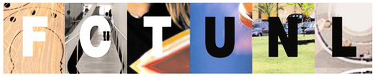
\includegraphics[width=8cm]{fctunlnlogo.jpg}
\end{minipage}


\vspace{0.75cm}
  
\begin{minipage}{7cm}
	\small
	\textbf{Centro de Inteligência Artificial}\\
	\textsl{Departamento de Informática} \\
  Faculdade de Ciências e Tecnologia \\
  \textbf{Universidade Nova de Lisboa}
\end{minipage}



\vspace{7cm}

\begin{minipage}{17cm}
  \LARGE
  \bfseries 
  \Huge Revising Undefinedness\LARGE \\in the Well-Founded Semantics of Logic Programs
\end{minipage}

\vspace{1cm}

{\large\bfseries Luís Filipe Rodrigues Soares}




\vfill


\begin{minipage}{10cm}
\footnotesize A thesis submitted to the Department of Computer Science and the Committee on Graduate Studies of Universidade Nova de Lisboa in partial fulfillment of the requirements for the degree of Master of Science\\
\\
Caparica, 2006
\end{minipage}



\clearpage


\vfill
\begin{flushright}
  This dissertation was prepared under the supervision of\\
  Professor Luís Moniz Pereira,\\
  of the Faculdade de Ciências e Tecnologia,\\
  Universidade Nova de Lisboa.\\[0.5cm]
\end{flushright}



\cleardoublepage


\thispagestyle{empty}
\begin{flushright}

\begin{minipage}{9cm}
\vspace{2.5cm}
\hfill%
\begin{tabular}[t]{r}
\emph{to the dropplets of}\\
\emph{water,}\\
\emph{bashing in the}\\
\emph{haul}\\
\emph{of an intense vessel,}\\
\emph{fading}\\
\emph{as life goes on;}\\
\emph{such are the}\\
\emph{difficulties and}\\
\emph{fears.}\\
\end{tabular}

\end{minipage}
\end{flushright}
\cleardoublepage


% =================================================================
%     Acknowledgements
% =================================================================
\selectlanguage{english}
\chapter*{Acknowledgements}



This thesis, completed within a year of very intense experiences, actually spans over the last three or four years of my life. Those were truly crucial years in setting the motivation for coming to Nova and persuing this line of work, now giving its first results. For this, I thank Isa. During all these years she always supported me and believed me, and without her company and encouragement this work wouldn't have happened. She was always available to listen to my wandering thoughts on logic and absurdity, as well as my concerns and fears regarding my work and its success. The moments I spent with her were always beautiful and full of joy and tranquility. Her love and friendship were the best strenghts I could have had to give this first step, and those are things that I \emph{always} keep with me. Thanks.

My mother and my sister are among the most patient persons in the world. They always let me do things my way, even when it interfered with their lives and schedules, and they always beared with my sudden special needs, even when this meant more work for them. My mother was specially inspiring in the way she has always fought everything without ever giving up, a beautiful persistence I'm sure I got from her.

On the academic side, Professor Moniz Pereira made this whole adventure possible. He was the kind of supervisor I wanted, always keeping me occupied with challenges and always available for my doubts and difficulties. The fact that he accepted me as his student and that he believed in my work was of the utmost importance to me. His constant dedication to scientific research is truly inspiring and his contagious sense of humor was essential for the completion of this thesis.

Thanks are also due to the Departamento de Inform�tica and the Centro de Intelig�ncia Artificial, for providing me with working conditions and great examples among the people working there. The Secretariat staff has always been helpful and patient in all the things I required, for which I also thank them. A special word of thanks also goes to the Multimedia and Databases Laboratories research group, at Escola Superior de Tecnologia, Instituto Polit�cnico de Set�bal, for providing me alternative working conditions.

I also have to thank my juri, Professor Carlos Dam�sio and Professor Carlos Caleiro, whose insights were more than essential for the final version of this work.

S�rgio, Carmen, Miguel, Hugo Silva and Jo�o Leite were of great help in proofreading my thesis, for which I thank them.

I have a great thank to give to S�rgio, who was always there to listen to me talking about my work, even though he had his own concerns with pixels, isosurfaces and volume rendering. He was one of the few people who actually understood this work, contributed with new problems and examples, even spent some time solving some of these issues and yet this had nothing to do with what he was working on. We spent some great relaxing moments in math's bar, just talking and enjoying the \emph{views}. Those \emph{views} were indeed crucial to our mental sanity. Thanks for being a great friend and formidable colleague.

Doca de Santo at Alc�ntara and Bar Pro�bido at Bel�m were alternative working places. Besides having good working environments, these were also relaxing places to escape from work.

Jo�o Leite was also of great help and inspiration ever since I came to Nova. These ideas weren't among his favourites and so our discussions were a great test to my persistence and my belief in my work, which I think only made it stronger. Besides, he was a great professor, a great research partner and an example both in achievements and dedication to his work.

A special thanks also goes to Sophie, who opened my eyes to a lot of important issues during this period of time. Our moments were filled with brevity but set many important things in motion regarding me and this thesis. We ended up sharing \emph{more} than just music, which had a great impact on me and my work.

Miguel, Mit� and Carmen were the greatest friends I could have had. Their companion, support and advices were more than essential to me. Carmen has accompanied me since I came to Nova and has always given me important advices, as well as great moments of fun, along with her big Vimi. Mit� was a fun companion in all the singing and guitar playing in her house and at Amadeu's. Not everyone could appreciate the greatness of our voices, which only means they are \emph{that} special. Miguel has probably interfered more with my life than any other person. He was my professor, my supervisor, my work partner and is something like a best friend and an older brother to me. He always had time and the moments I spent in his company were always enjoyable and relaxing. Besides all this, he has always been an inspiration in so many ways. Thank you for always being there.

%\vspace{1cm}
And finally there is Maria, who has (a)mused me when I needed it the most, and gave me so many crazy and passionate moments; an intensity I was missing and which I truly needed. Thanks.
% =================================================================
%     Summary
% =================================================================
\selectlanguage{english}
\chapter*{Summary}

The \WFS(WFS) for \nlps associates with each program one single model expressing truth, falsity and undefinedness of atoms. Under the WFS, atoms are said to be undefined if:

\begin{itemize}
	\item Either are part of a two-valued choice (true in some worlds, false in others) but never undeniably true or false;
	\item Or are not classically supported;
	\item Or depend on an already undefined literal, as in one of the previous cases.
\end{itemize}

Undefinedness due to lack of classical support could be overcome by the introduction of another form of support, which would allow the WFS to deal with programs requiring other forms of reasoning besides the classical support, and thus gain expressiveness. One of these forms of support whose application has already been studied in the \RSMs semantics (rSMs) is support by \raa (RAA). This principle states that an hypothesis should be true if by assuming it's false this assumption leads to a contradition.

In this thesis we propose to study the application of the RAA principle to the WFS, thus defining the \RWFS (RWFS). Besides this definition we'll also study the definition of a fixed-point operator $\Gamma^{r}$, a counterpart of \GFo $\Gamma$, with support for RAA reasoning, and use this operator to perform the calculation of rSMs and the \rwfm of \nlps. We will also study a new property of rSMs and the definition of the \rpsms.

This thesis concludes with the discussion of several open issues and possible next research paths.



% =================================================================
%     Sum�rio
% =================================================================
%%\selectlanguage{portuges}
\chapter*{Sum�rio}

A Sem�ntica Bem-Fundada (SBF) dos programas l�gicos normais associa a cada programa um �nico modelo que expressa a verdade, falsidade e indefini��o dos seus �tomos. Os �tomos, na SBF, dizem-se indefinidos se:

\begin{itemize}
	\item Ou s�o parte de uma escolha a dois valores (verdadeiros em alguns mundos, falsos noutros) mas nunca s�o inquestionavelmente verdadeiros ou falsos;
	\item Ou n�o t�m suporte cl�ssico;
	\item Ou dependem de �tomos que j� s�o indefinidos, por um dos casos anteriores.
\end{itemize}

A indefini��o devida � falta de suporte cl�ssico pode ser ultrapassada atrav�s da introdu��o de outra forma de suporte, o que permitiria � SBF lidar com programas l�gicos normais de acordo com outras formas de racioc�nio para al�m do suporte cl�ssico, ganhando desta forma expressividade. Uma destas formas de racioc�nio cuja aplica��o foi j� estudada na sem�ntica dos Modelos Est�veis Revistos (MERs) � o suporte por \emph{redu��o ao absurdo} (RAA). Este princ�pio diz que uma hip�tese dever� ser verdadeira se, por causa de se assumir que ela � falsa, essa assump��o nos leva a uma contradi��o.

Nesta tese prop�mo-nos a estudar a aplica��o do princ�pio de RAA na SBF, definindo assim a Sem�ntica Bem-Fundada Revista. Para al�m desta defini��o, vamos tamb�m estudar a defini��o de um operador de ponto fixo $\Gamma^{r}$, que ser� a vers�o com suporte por RAA do operador Gelfond-Lifschitz $\Gamma$, e vamos usar este operador para calcular os MERs e o modelo bem fundado revisto de programas l�gicos normais. Vamos ainda estudar uma nova propriedade dos MERs e a defini��o dos modelos est�veis revistos parciais.

Esta tese culminar� com uma discuss�o de v�rios pontos em aberto e do trabalho futuro a realizar neste contexto.


% =================================================================
%     Return to english as the main language
% =================================================================
\selectlanguage{english}

\incrementmtc

%% =================================================================
%     Symbols
% =================================================================
\chapter*{Symbols}


% =================================================================
% Local variables:
% TeX-master: "../tese.tex"
% End:
% =================================================================



\tableofcontents
%\listoffigures
%\listoftables


\mainmatter


%%%%% page numbers again

\pagestyle{fancy}
\fancyhead{}
\fancyhead[RO,LE]{\leftmark\hfill\rightmark}
\renewcommand{\chaptermark}[1]{\markboth{\fontfamily{phv}\selectfont\footnotesize
    \thechapter.\ \textsc{#1}}{}}
\renewcommand{\sectionmark}[1]{\markright{\fontfamily{phv}\selectfont\footnotesize\thesection.\ #1}}
\pagenumbering{arabic}




%%%%%%%%%%%%%%%%%%%%%%%%%%%%%%%%%%%%%%%%%%%%%%%%%%%%%%%%%%%%%%%%%%%%%%%%%%%%%%%%%%
%%%%
%%%%        THE CHAPTERS
%%%%
%%%%%%%%%%%%%%%%%%%%%%%%%%%%%%%%%%%%%%%%%%%%%%%%%%%%%%%%%%%%%%%%%%%%%%%%%%%%%%%%%%


%%#################################################################
%% CHAPTER 1.
%%#################################################################
\chapter{Introduction}
\label{cha:introduction}


\begin{ChapAbstract}
Where we briefly present the motivational setting for this thesis, the problems we intend to address and the main contributions of this work. In this chapter we also outline the structure and contents of each chapter.
\end{ChapAbstract}
	
\vspace*{0,5cm}
\begin{flushright}
	\begin{tabular}{l}
		\small \textsl{I know, I know for sure,}\\
  	\small \textsl{That life is beautiful around the world (\ldots)}\\
		\hline
		\scriptsize Red Hot Chili Peppers. Around the World. In \textsl{Californication}.\\
  	\scriptsize Warner Bros., 1999.
	\end{tabular}
	
\end{flushright}

\vspace*{1,5cm}

\section{Motivation}
\label{sec:motiv}
The concerns of what was known for sure were among the things that puzzled Anthony Kiedis of the Red Hot Chili Peppers, whether these concerns were with how life was around the world or what to say to a girl when she says ``Hello\ldots''\cite{californication}. To know these things for sure would imply that he had analyzed every relevant fact and rule regarding the beauty of life around the world (and conversations with girls) and, given one single observation of the world, he would be able to conclude what was true or false, and what was impossible to say if it was true or false. This single view would be skeptical, cautionate in the way it attributed truth or falsity to things. And for those cases where things weren't absolutely true or false, this view would say that things should be undefined.

Undefinedness helps enforcing a skeptical view of the world. It's a truth value used to refer to things whose truthness can't be determined. Things fall in this category, for example, when there are situations in which a certain thing is true, and other situations where the same thing is false. Things might also fall in this category when, for some reason the truth value of something just can't be determined or things depend on already undefined things. In either case it's more cautious to say that things are undefined than to compromise with truth or falsity.

The reasoning behind this idea was captured under a precise semantics for logic programs, around 1990. The \WFS\cite{wfsMain}(WFS) has several desirable properties as a semantics for logic programs, namely cumulativity, relevancy and existence. Furthermore, it ensures uniqueness of model, its \wfm is computable in polynomial time and several WFS implementations (\cite{xsbSite,xsbArticle,branchBound,alternatingFixpoint}) have been studied and exist nowadays. Moreover, several important relations exist between the \wfs and \nmr formalisms\cite{wfsDualities,wfsGeneralized}, as well as between the \wfs and the \sms semantics\cite{wfsCoincides,wfsRelation}, another important semantics for \nmr. Additionally, the WFS was later expanded to its explicit\cite{jjaPhD,wfsxArticle}, paraconsistent\cite{paraconsistentArticle} and disjunctive\cite{alcantaraPhD} counterparts.

Under the \wfs, atoms can be true, false or undefined. They are said to be true if and only if they are undoubtfully true, i.e., they have classical support and when transitioning to a two-valued context with several (possible) models, they are true in all models. Literals are said to be undefined if they fall in one of the following cases:

\begin{itemize}
	\item Either they are part of a two-valued choice (true in some worlds, false in others) but never undeniably true or false;
	\item Or they are not classically supported;
	\item Or they depend on an already undefined literal, as in one of the previous cases.
\end{itemize}

Otherwise, they are false.

It's easy to see that literals that are part of choices should be undefined -- choices are made in a two-valued context so things are either true or false. In a three-valued context, as they can't be true and false at the same time they remain undefined. 

For this consider the example:
\begin{align*}
P=\{& a \leftarrow not b\\
		& b \leftarrow not a\}
\end{align*}

The \wfm of $P$ is empty, with both $a$ and $b$ being undefined. This is so because when $a$ is true $b$ is false, and vice-versa.

Additionally, if a literal depends on an already undefined literal it should also be undefined\footnote{Although it can be argued that, in some cases, some conclusions may be derived from literals which already were undefined, namely when we are referring to choices. We dedicate some attention to this possibility in the conclusions.} -- undefinedness propagates throughout the program. 

As an example, consider:
\begin{align*}
P=\{& a \leftarrow not b\\
		& b \leftarrow not a\\
		& c \leftarrow a\\
		& c \leftarrow b\}
\end{align*}

The program has two stable models, $SM_{1}=\{a,c\}$ and $SM_{2}=\{b,c\}$, and the stable models semantics of the program is $\{c\}$, which is the intersection of its models. However, this does not correspond to the WFS; even though $c$ is true in all two-valued worlds (according to the \sms) it depends on undefined literals and as such it is also undefined.

Finally, we have a case with a literal which has no classical support in the sense that the conclusions are supported by a set of premises:
\begin{align*}
P=\{& a \leftarrow not a\}
\end{align*}

$a$ depends on its own negation, which is not a valid premise as it would lead us to a contradiction. Therefore the WFM of this program is empty, with $a$ being undefined. However, lack of classical support could be overcome with the introduction of another form of support or with an extension to classical support, as in the case of the principle of \RAA\footnote{It has generated some controversy whether or not the principle of \raa should be considered a classical form of reasoning. We will deal with this question in greater detail in chapter \ref{cha:rwfs} leaving for now the idea that in the context of this thesis we will consider the RAA principle a nonclassical form of support.}. This will be the theme of this thesis.



\section{Approach}
As we stated before, it's easy to see that literals that are part of choices should be undefined, as well as those that are dependent on atoms which already are undefined. Lack of classical support, however, could be overcome by the introduction of another form of support. By enabling other forms of support, the WFS would gain expressiveness and the ability to correctly deal with programs which required non-classical forms of reasoning. One such program is the following:
\begin{align*}
P=\{ & go\_out\_with\_me\leftarrow sad\\
		 & sad \leftarrow not\text{ }go\_out\_with\_me\}
\end{align*}

This program represents one possible reasoning behind asking a girl out on a date. What the program is stating is that she should go out with me\footnote{Without loss of generality\ldots} if she is sad. Furthermore, she will be sad if doesn't go out with me. Under this scenario, and given that the girl in question doesn't want to be sad, she could start by questioning herself, for instance, what would happen if she refused the invitation. By assuming the hypothesis $not\text{ }go\_out\_with\_me$, she should be sad. However, being sad is precisely the precondition for ``going out with me'', contradicting the original hypothesis. Therefore, she couldn't refuse the invitation -- she would ``go out with me''.

The reasoning behind this program is not a classical one, in the sense that the conclusions don't actually depend on a set of true premises -- they depend on the impossibility of one of the negated premises being false, as this falsity would be contradictory with respect to the conclusion. The literal $go\_out\_with\_me$ is actually concluded by reasoning by absurdity, a form of \emph{unclassical} support. However, as the \wfs doesn't employ this kind of support, both atoms $\{go\_out\_with\_me, sad\}$ would be undefined in the \wfm. Let's consider another example, still in the same context:
\begin{align*}
P=\{ & go\_out\_with\_me\leftarrow sad\\
		 & sad \leftarrow not\text{ }go\_out\_with\_me,\text{ }not\text{ }get\_drunk\\
		 & get\_drunk\leftarrow bored\\
		 & bored \leftarrow not\text{ }get\_drunk\}
\end{align*}

Under this program, we are stating that the previous girl will be sad not only if she doesn't go out with me, but also if she doesn't get drunk. Regarding the ingestion of alcoholic drinks, she will usually get drunk if she is bored. However, she will get bored if she is not drunk. Following the reasoning behind the previous example, this girl will always be drunk. This state will prevent her from being sad and, therefore, of going out with me. Once again, under the \wfs, all atoms will be undefined. However, if we were able to reason by absurdity in the WFS, we would conclude $drunk$, while everything else would be false.

This \emph{reasoning by absurdity} follows the principle of \raa (RAA), which states that an hypothesis should be true if by assuming it is false this assumption leads to a contradiction. In that case, our conclusion is that our hypothesis should be true. 

The application of this principle has already been studied in the \SMs Semantics\cite{smMain} (SMs) and enabled the \RSMs\cite{ampMSc,rsmEpia} (rSMs) to solve the problems associated with the SMs, while also enjoying the advantages associated with them. It also provided with an initial proof that the principle of RAA could effectively be used as a form of \emph{unclassical} support. 


Studying the application of this principle in the \wfs will be the subject of this thesis.


\section{Contributions and Outline}
In this thesis we propose to study and implement the application of the \raa principle to the \wfs, with the purpose of contributing with more expressive results in a three-valued context, by recurring to undefined only when dealing with choices or with propagation. The study of the application of the RAA principle in the WFS will also provide a way of transitioning between a three-valued semantics with RAA support and the the \rsms, these also sharing the same form of \emph{unclassical} support. We will dub this semantics the \RWFS (rWFS) and study the definition and calculation of its \RWFM (rWFM).

The introduction of this semantics further provides the following contributions:

\begin{itemize}
	\item The study of the application of the principle of \raa in a three-valued scenario, as well as the implications this introduction would have when defining a semantics based in this principle;
	\item The definition of the principle of \raa in a three-valued context, which is an extension of the original principle, only valid in a two-valued context;
	\item The definition and brief study of the \rpsms, a complete counterpart of the \psms, where the path between the rWFM and the rSMs always exists and is only the result of choices on undefined literals;
	\item The study of RAA patterns and the consequent definition of a fixed-point operator $\Gamma^{r}$ which is the counterpart of the \GFo $\Gamma$, with support for RAA reasoning;
	\item The definition of the \rsms semantics and the \rwfs through the use of \gro, and other further explorations in the \rsms semantics.
\end{itemize}


This thesis is organized as follows: Chapter \ref{cha:SoA} presents the historical and theoretical settings of this work and discusses the achievements of the three most relevant semantics in the context of this thesis. It ends with an account of the role played by each semantics and what role the rWFS should play.

In Chapter \ref{cha:rwfs} we define the \rwfs. We start with an extensive motivation for the introduction of this semantics and we define the principle of RAA in a three-valued setting. We then provide several preliminary definitions which will enable us to contextualize the RAA principle and present the declarative definition of the rWFS. We then study its properties and present some examples of the calculation of the \rwfm.

In chapter \ref{cha:grExtension} we start with a new property of the \rsms, RAA rule extension, which will enable us to define a syntactic transformation for rSMs and the rWFS. After defining this transformation we present some programs and the calculation of their \rsms and \rwfm.

This thesis ends with a discussion of some open issues and concluding remarks.
       % Introduction
%%#################################################################
%% CHAPTER 2
%%#################################################################
\chapter{History and Theoretical Foundations}
\label{cha:SoA}

\begin{ChapAbstract}
Where we present the historical and theoretical context for this thesis. We briefly present the sequence of events which resulted in this thread of research, and present the main definitions and base concepts needed to understand this work.
\end{ChapAbstract}


\section{A Historical Overview}
The field of Artificial Intelligence\footnote{As one would expect, only part of the last fifty years are addressed in these brief paragraphs, in particular those that are relevant for this thread of research in Artificial Intelligence.} (AI) has grown in both depth and breadth since its very name was coined at the 1956 Dartmouth College meeting\cite{dartmouth}. If, in those early days, AI was hardly considered a science, it didn't take long for formal methods of research and development to appear. The area soon became richer in its various approaches to the challenge of providing computers with methodologies similar to those used by humans to solve problems.

From the several approaches that followed the Dartmouth meeting regarding knowledge representation, one was related with the use of logical formulas to express knowledge. It was around 1960 that John McCarthy first expressed the advantages of such approach\cite{commonSense}:

\begin{quotation}
``Expressing information in declarative sentences is far more modular than expressing it in segments of computer programs or in tables. Sentences can be true in a much wider context than specific programs can be used. The supplier of a fact does not have to understand much about how the receiver functions or how or whether the receiver will use it. The same fact can be used for many purposes, because the logical consequences of collections of facts can be available.''
\end{quotation}

Other authors defended this orientation, namely Patrick Hayes\cite{philoProblems}, Nils J. Nilsson\cite{logicAI} and Drew McDermott\cite{critique}, which ended up originating two main threads of research, initially very distinct but later converging on the same line of work.

The first of these was Logic Programming (LP). Logic Programming, the application of automatic methods of deduction combined with logic-based knowledge representation, was started by Alain Colmerauer \cite{prologReport} and Robert Kowalski\cite{logicAlgorithmControl,kowalskiPredicate}, and introduced in Computer Science the idea of a declarative logical approach to programming, as opposed to a procedural one. This new programming paradigm was summarized by Robert Kowalski in \cite{logicAlgorithmControl}, and ended up providing a fast proliferation of the logic-based approach to AI, as researchers now had a way to implement and test their theories. Logic programming eventually came to life under the Prolog\footnote{Prolog is an abbreviation of \emph{PROgrammation en LOGique}, name suggested by Philippe Roussel\cite{birthProlog}.} language in 1972 by the hand of Colmerauer and Kowalski, which not only did it demonstrate that Prolog was a practical language as it also helped disseminate it worldwide. Nowadays several Prolog distributions exist, making LP a relevant paradigm in Computer Science.

During the same years, other researchers were delving into the problems of performing commonsense reasoning in AI. John McCarthy was perhaps the first person to consider these issues\cite{commonSense} and later, together with Patrick Hayes\cite{philoProblems}, introduced the Frame Problem. The Frame Problem deals with the representation of things that do not change in a given situation, when a certain event occurs. This frame problem was precisely the kind of problem to be addressed by nonmonotonic reasoning, the fact that monotonic classical logic \emph{per se} does not deal correctly with changing worlds. The term \emph{nonmonotonic reasoning} is probably attributed to Marvin Minsky in \cite{nmrTermIntroduction}, where he also summarizes his critique to classical logic. 

Both threads of research continued to evolve rather separated from each other, until 1986. In 1986, at the Workshop on the Foundations of Deductive Databases and Logic Programming, a major milestone was reached with the Stratified Semantics -- it is a semantics of interest for the LP community, but its underlying principles are more closely related to those of NMR. It was a milestone precisely because this and the group of semantics that followed, left the operational concerns of classical LP behind and were more concerned with their suitability for practical applications and NMR. 

During the following years, several different semantics appeared and important relations between them and NMR were discovered. Of particular interest to this work are the following moments:

\begin{itemize}
	\item 1988, introduction of the Stable Models Semantics\cite{smMain};
	\item 1991, introduction of the Well-Founded Semantics\cite{wfsMain};
	\item 2004, introduction of the Revised Stable Models Semantics\cite{ampMSc, rsmEpia}.
\end{itemize}

These semantics set the grounds for this work and constitute the last steps in the thread of research we have described so far.

In the remainder of the chapter, we'll introduce the theoretical notions required for the understanding of this work, as well as the semantics it is based on. We end up with a motivation for the \rwfs, the main theme of this thesis.


\section{Language of Logic Programs and Other Common Definitions}
We now present the theoretical context for this thesis by showing several basic definitions that will be used throughout this work.

We start by defining an alfabet\footnote{The definitions in this section are borrowed and extended from \cite{aparasPhD,jjaPhD,milkBook}.} $\cal{A}$ over a language $\cal{L}$, which is a finite or countably infinite disjoint set of constants, predicate symbols with associated arity, function symbols with associated arity, as well as a countably infinite set of distinguished variables.


\begin{definition}[Term]
A term over $\cal{A}$ is defined as one of the following:
\begin{itemize}
	\item A variable, which we'll normally write as $X$, in uppercase;
	\item A constant, which we'll normally write as $x$, in lowercase;
	\item A function symbol $f(t_{1},\ldots,t_{n})$ with $t_{1},\ldots,t_{n}$ being terms;
\end{itemize}
A term is said to be ground if it doesn't contain variables.
\end{definition}

\begin{definition}[Atom]
An atom is either a term or an expression $p(t_{1},\ldots,t_{n})$, where $p$ is a predicate symbol and $t_{1},\ldots,t_{n}$ are terms. An atom is ground if all its terms are grounded.
\end{definition}

\begin{definition}[Herbrand base]
The set of all ground atoms is called the Herbrand base and is represented as $\cal{H}$.
\end{definition}

\begin{definition}[Literal]
A literal is either an atom $A$ or its default negation $\sim A$. 
We will use the symbol $\sim$ to refer to the implicit negation, or default negation. Hence, literals can also be called positive literals or default (negative) literals, whether they are respectively non-negated literals or negated literals.
A literal is said to be ground if it doesn't contain any variable.
\end{definition}

\begin{definition}[Rule]
A rule is a clause over $\cal{A}$ in the form
\begin{align*}
H\leftarrow A_{1},\ldots,A_{n}
\end{align*}
where $H$ is a positive literal and $\{A_{1},\ldots,A_{n}\}$ are positive or negative literals. $H$ is called the head of the rule while $\{A_{1},\ldots,A_{n}\}$ constitutes the body of the rule. If a rule doesn't contain a body it is called a fact and is represented as 
\begin{align*}
H\leftarrow 
\end{align*}
\end{definition}

\begin{definition}[Heads and Bodies of rules]
Regarding rules we define the functions $head(r)$ and $body(r)$ which, for any rule $r$ respectively give as a result its head and its body.

Given a set of rules $S$, the functions $heads(S)$ and $bodies(S)$ respectively give as a result the set of all heads of all rules of $S$ and the set of all bodies of all rules of $S$.
\end{definition}


From these definitions we can now specify what we mean by a \DefP and a \NLP.

\begin{definition}[\DefP]
A \defp (DP) $P$ is a countable set of rules, such that their bodies only include positive literals.
\end{definition}

\begin{definition}[\NLP]
A \nlp (NLP) $P$ is a countable set of rules.
\end{definition}

The transition from NLPs, which are only syntactic descriptions of some world or situation, to the meaning they have is done through the following definitions regarding interpretations and models.


\begin{definition}[Two valued Interpretation]
A \twovi $I$ of a NLP $P$ is any subset of the Herbrand base $\cal{H}$ of $P$, and can be viewed as the set
\begin{align*}
I=\cal{T}\cup\sim \cal{F}
\end{align*}
where $\cal{T}\subseteq I$ is the set of ground atoms true in $I$ and $\cal{F}=\cal{H}\setminus \cal{T}$ is the set of ground atoms false in $I$.
\end{definition}

\begin{definition}[Three valued Interpretation]
\label{def:threeVI}
A \threevi $I$ of a NLP $P$ is a set
\begin{align*}
I=\cal{T}\cup\sim \cal{F}
\end{align*}
where $\cal{T}$ and $\cal{F}$ are disjoint sets of the Herbrand base $\cal{H}$ of $P$ and $\cal{T}$ is the set of ground atoms true in $I$ and $\cal{F}$ is the set of ground atoms false in $I$. The truth value of the remaining ground atoms is undefined.
\end{definition}

For the sake of simplicity, we'll often refer to two-valued interpretations only by including the set of atoms that are true ($\cal{T}$), and \threevi by including the set of atoms which are true, and those which are true or undefined as a tuple $\langle\cal{T},\cal{TU}\rangle$.

Interpretations can be viewed as \emph{possible worlds} of a program $P$, as it is discussed by Przymusinska and Przymusinski\cite{semanticIssues} which correspond to possible states of knowledge regarding program $P$. Three valued interpretations account for the possibility of not knowing everything about the world, and being able to represent the things known to neither be definitely true nor definitely false.

\begin{definition}[Satisfaction]
Given an interpretation $I$ (two valued or three valued) and a NLP $P$ we say that:
\begin{itemize}
	\item $I$ satisfies a literal $X$, denoted by $I\models X$, iff $X\in I$;
	\item $I$ satisfies the conjunction $X_{1},\ldots,X_{n}$, denoted by $I\models \{X_{1},\ldots,X_{n}\}$, iff $I\models X_{1},\ldots,I\models X_{n}$;
	\item $I$ satisfies the rule $H\leftarrow X_{1},\ldots,X_{n}$, denoted by $I\models (X_{1},\ldots,X_{n})$, iff whenever the conjunction $X_{1},\ldots,X_{n}$ is satisfied by $I$, then $H$ is also satisfied by $I$.
\end{itemize}
\end{definition}



\section{Stable Models Semantics and the Well-Founded Semantics}
Gelfond and Lifschitz introduced the \SMs Semantics (SMs) in 1988\cite{smMain}, a semantics which would end up becoming one of the most important in the field of logic programming. 

The main idea behind the \sms comes from the field of \nmr, following the sequence of events detailed in the previous section. Its intuition is that if we assume some literals as true and others as false, those assumptions should be corroborated by the semantics of definite programs\cite{predicateProgramming}. If they are, then they form a stable model. This semantics makes use of an operator that, given a \twovi $I$, transforms the NLP into a definite program (DP), in order to calculate its least model.

\begin{definition}[\GFo $\Gamma$]
Let $P$ be a NLP and $I$ a \twovi. The GL-transformation of $P$ modulo $I$ is the program $\frac{P}{I}$ obtained from $P$ by performing the following operations:

\begin{itemize}
	\item Remove from $P$ all rules containing a default literal $\sim X$, such that $X\in I$;
	\item Remove from the remaining rules all the other default literals.
\end{itemize}

Since $\frac{P}{I}$ is a DP, it has a unique least model $J$.

Let $\Gamma_{P}(I)=J$.
\end{definition}



\begin{definition}[\SMs Semantics]
A \twovi $I$ of a NLP $P$ is a Stable Model of $P$ iff $\Gamma_{P}(I)=I$.

A ground atom $X$ of $P$ is true under the \sms semantics iff $X$ belongs to all stable models of $P$.

We represent a \sm $M$ of a NLP $P$ as $SM_{P}(M)$.
\end{definition}

It was soon discovered\cite{bidoit,gelfondStratified} that the \sms are closely related to \nmr formalisms, namely Reiter's default extensions\cite{reiterDefault} and Moore's autoepistemic extensions\cite{mooreAutoepistemic}. This close relation helped bring the fields of \NMR and Logic Programming closer, by providing LP with \nmr formalisms and NMR with a practical vehicle of experimentation and research.

Besides this important relation, the SMs ended up being defined for the extended class of logic programs, i.e., logic programs with classical negation. The resulting semantics, the Answer Set Semantics\cite{answerSets} is one of the most used in Multiagent Systems and Artificial Intelligence applications where the knowledge representation approach based on logic.

The SMs have, however, some important drawbacks. First of all, the \sms semantics is not always consistent, which means that some programs have no semantics at all. Consider, for example 
\begin{align*}
P=\{a&\leftarrow\sim a\}
\end{align*}

$\Gamma_{P}(\{a\})=\{\}$ but $\Gamma_{P}(\{\})=\{a\}$, which means $P$ has no semantics whatsoever, because there is no single interpretation $I\subseteq{\cal{H}}_{P}$ such that $\Gamma_ {P}(I)=I$. Additionally, the SMs also lack the properties of Cumulativity (the addition of lemmas from a model to the original program doesn't alter the semantics) and Relevancy (the possibility of implementing a top-down query-driven proof-procedure), and its computation, even brave-reasoning, is NP-Complete\cite{npComputation}.

Three years passed since the introduction of the SMs until Alan van Gelder along with Kenneth Ross and John Schlipf proposed\cite{wfsMain} the Well-Founded Semantics (WFS). The WFS overcomes all the problems described before and still maintains a strong relation with NMR formalisms. It is more expressive than the \sms semantics as it uses three-valued interpretations but is also a lot more skeptical, attributing the value of undefined to all those literals which are not undoubtfully true or false (or depend on ones who are, in turn, undefined), or lack classical support.

Several definitions of the \wfs exist in the literature. For this work, we'll make use of the one defined by Baral and Subrahmanian\cite{wfsDualities}, which is most closely related with our approach to the subject of this thesis.

\begin{definition}[\BSo $\Gamma^{2}$]
Let $P$ be a NLP and $I$ an two-valued interpretation. The \BSo $\Gamma^{2}$ is defined as being two applications of the \GFo $\Gamma$:
\begin{align*}
\Gamma_{P}^{2}(I) = \Gamma_{P}(\Gamma_{P}(I))
\end{align*}
\end{definition}

\begin{definition}[\WFS]
Let $P$ be a NLP. The \WFS of program $P$ is the tuple $\left\langle \cal{T},\cal{TU} \right\rangle$, with $\cal{T}$ corresponding to the true literals according to the semantics and $\cal{TU}$ being the true or undefined literals according to the semantics.

The $\cal{T}$ set can be calculated as being the least fixed point of $\Gamma_{P}^{2}$ starting with the empty interpretation, i.e., $\cal{T}=$$\Gamma_{P}^{2\text{ }\uparrow \omega}(\{\})$, with $\omega$ being the least limit ordinal.

The $\cal{TU}$ set can be calculated as being the next iteration of $\Gamma_{P}$, starting from the $\cal{T}$ set, i.e., $\cal{TU}=$$\Gamma_{P}(\cal{T})$.

We will refer to the \wfm $M$ of any NLP $P$ as $WFM_{P}(M)=\langle\cal{T},\cal{TU}\rangle$. The $\cal{T}$ set of the WFM will be referred to as \tWFM and the set $\cal{TU}$ of the WFM will be referred to as \tuWFM.
\end{definition}

The \wfs has all the properties the \sms miss, namely cumulativity, relevancy and existence. Furthermore, it ensures uniqueness of model, a property desirable for the \wfs. Its \wfm is computable in polynomial time and several WFS implementations (\cite{xsbSite,xsbArticle,branchBound,alternatingFixpoint}) have been studied and exist nowadays. Moreover, several important relations exist between the \wfs and \nmr formalisms\cite{wfsDualities,wfsGeneralized}, as well as between the \wfs and the \sms semantics\cite{wfsCoincides,wfsRelation}. Additionally, the WFS was later expanded to its explicit\cite{jjaPhD,wfsxArticle}, paraconsistent\cite{paraconsistentArticle} and disjunctive\cite{alcantaraPhD} counterparts. It falls out of the scope of this thesis to analyse and comment on these relations; the key subject here is that the WFS ended up being heavily studied.

During the last decades, these two semantics were extensively used and studied for \nmr and \kr. The \sms semantics on one side, when researchers needed a two-valued semantics, capable of representing several possible worlds as models of a program; and the \wfs on the other side, when researchers were willing to sacrifice the expressiveness of having multiple two-valued models in order to have a three-valued skeptical and sure-footed semantics.


\section{Enter the \RSMs}
The drawbacks of the \sms semantics, described in the previous section, are dealt with in the \wfs but they aren't actually \emph{solved}. Only in 2004 Pinto and Moniz Pereira proposed\cite{rsmItaly} a way of solving the problems of the \sms and have been studying\cite{ampMSc,rsmEpia,rsmItaly} its aspects ever since.

The Revised Stable Models (rSMs) is a semantics for NLPs which applies the principle of \RAA (RAA) to solve the main problems of the \sms semantics, namely inconsistency, cumulativity and relevancy. Inconsistency in SMs, as it was shown by François Fages\cite{fages}, comes from the existence of \olons (OLONs) in the program such as
\begin{align*}
P=\{a\leftarrow\sim a\}
\end{align*}

François Fages goes on explaining that not only OLONs are the source of the problem for inconsistency, but also \icons (ICONs), as in the case of:
\begin{align*}
P=\{& p(X)\leftarrow p(s(X))\\
& p(X)\leftarrow\sim p(s(X))\}
\end{align*}

In a nutshell, according to the principle of \raa if a certain hypothesis leads to a contradiction, it should be withdrawn. In the first case, by assuming $\sim a$ as true, this assumption will eventually lead us to conclude $a$, a contradiction. Therefore $\sim a$ cannot be concluded, so $a$ should be. In the second case, if we assume $\sim p(X)$ then the bodies of both rules should be false, which is impossible since they are logical oppositions. Therefore, $p(X)$ must be true, as $\sim p(X)$ will never be.

\RSMs are in everything similar to the \sms, only changing the way the semantics deals with OLONs and ICONs -- it solves them using RAA reasoning, given that the conclusions derived from this resolution keep consistent with the rest of the program. This results in an extension to the \sms semantics, which solves all the problems detailed previously.


\begin{definition}[Sustainable Set\cite{ampMSc,rsmEpia}]
\label{def:sustainable}
As a shorthand notation only for this definition, let $WFM(P)$ denote the positive atoms of the Well-Founded Model of $P$, that is WFM(P) is the least fixed point of operator $\Gamma_{p}^{2}$\cite{wfsDualities}, i.e., $\Gamma_{p}$ applied twice. Intuitively, we say a set $S$ is sustainable in $P$ if and only if any atom $A$ in $S$ does no go against the well-founded consequences of the remaining atoms in $S$ whenever $S\setminus\{A\}$ itself is a sustainable set. The empty set by definition is sustainable. ``Not going against'' means that atom $A$ cannot be false ($A$ is true or undefined) in the well-founded model of $P\cup S\setminus\{A\}$, i.e., it belongs to set $\Gamma_{P\cup S\setminus\{A\}}(WFM(P\cup S\setminus\{A\}))$

Formally we say $S$ is sustainable if and only if:

\begin{center}
\begin{math}
\forall_{A\in S}, S\setminus\{A\}\ is\ sustainable\Rightarrow A\in \Gamma_{P\cup
S\setminus\{A\}}\left(WFM\left(P\cup S\setminus\{A\}\right)\right)
\end{math}
\end{center}

If $S$ is empty the condition is trivially true.
\end{definition}


\begin{definition}[Revised \SMs and Semantics\cite{ampMSc,rsmEpia}]
\label{def:rsms}
Let $RAA_{P}(M)\equiv M\setminus\Gamma_{P}(M)$. $M$ is a Revised Stable Model of an Normal \LP $P$, if and
only if:
\begin{itemize}
\item $M$ is a minimal classical model, with ``$\sim$'' interpreted as classical
negation;
\item $\exists_{\alpha\ge 2}$ such that $\Gamma_{P}^{\alpha}(M)\supseteq
RAA_{P}(M)$
\item $RAA_{P}(M)$ is sustainable.
\end{itemize}

The Revised \SMs semantics is the intersection of its models, just as in the \sms semantics.

We represent a \rsm $M$ of a NLP $P$ as $rSM_{P}(M)$.
\end{definition}

As it was proven in \cite{ampMSc}, the \rsms enjoy not only the existence of model property, therefore loosing the inconsistency the SMs had, as well as the properties of cumulativity and relevancy. They also served as a preliminary proof that the principle of \raa could be used as an additional form of support, which is a very important result for the context of this thesis.


\section{The Next Step}
This semantics and the additional notion of support it employs, somewhat change the map of \kr and \nmr semantics we have detailed so far.


\begin{figure}[htbp]
	\centering
		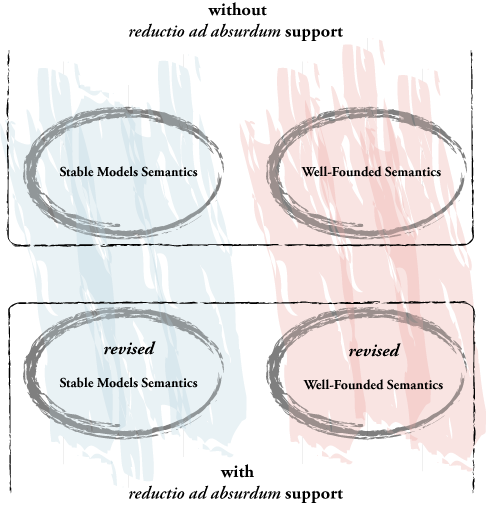
\includegraphics[width=0.55\textwidth]{Chap2/transitions.png}
	\caption{\footnotesize Map of transition and relations between the existing semantics for \nlps. Note that in the blue area, on the left, we have two-valued semantics while in the red area, on the right, we have the three-valued semantics. Additionally, the bottom of the figure represents semantics with RAA support, while the top of the figure represents those without RAA support.}
	\label{fig:transitions}
\end{figure}



The top level of figure \ref{fig:transitions} represents the current state of the art in semantics for \nlps \emph{without} RAA support. The \sms represent a flexible two-valued semantics, capable of representing several possible worlds in its various models. The \wfs represents a single three-valued view of a \nlp, enjoying several important properties but being too skeptical in its conclusions. The bottom level of the figure represents the corresponding semantics employing the principle of \raa as an additional form of support. The \rsms solve all the problems the \sms had, becoming a semantics as flexible as the SMs, with some of the properties the WFS had. All it's missing to define is the \RWFS, a three-valued counterpart of the rSMs and the next transition point from the WFS, when using the RAA notion of support.

In the next chapter we'll discuss the motivation for the definition of a rWFS, and continue providing its declarative definition. We'll then discuss the properties it enjoys when compared with the WFS and present some examples of its calculation.
       % State of the Art
%#################################################################
%% CHAPTER 3.
%%#################################################################
\chapter{Revised Well-Founded Semantics}
\label{cha:rwfs}

\begin{ChapAbstract} 
Where we propose the \RWFS and explore its properties. We present a declarative definition, relate it with previous concepts and semantics, and show some basic examples of its calculation. Most of the results in this chapter are then further explored in chapter \ref{cha:grExtension}.
\end{ChapAbstract}




%%%%%%%%%%%%%%%%%%%%%%%%%%%%%%%%%%%%%%%%%%%%%%%%%%%
%%%%%%%%%%%%%%%%% SECTION
%%%%%%%%%%%%%%%%%%%%%%%%%%%%%%%%%%%%%%%%%%%%%%%%%%%

\section{A Motivation for the \RWFS} 
\label{sec:motivRWFS}
As we've discussed in the previous chapter, we have three main semantics available for reasoning with \nlps, relevant for the context of this work. Two of these semantics (SMs and WFS) complement each other, by offering different levels of expressiveness and skepticism and by allowing an acceptable transition between two-valued and three-valued models. The other one (rSMs), extends the \sms semantics by introducing a new notion of support (\raa) in \nlps and thus solving the problems the SMs had. We now discuss the motivation for the introduction of a \rwfs, by identifying the main problems it should solve and the additional properties it will bring to the family of semantics with RAA support.

As we've seen, unlike the \sms semantics, the \wfs is well defined for all \nlps. Every \nlp has a \wfm that specifies its meaning with three truth values where it states the truth, falsity and undefinedness of literals. Under the WFS, atoms are said to be true if and only if they are undoubtfully true, i.e., they have classical support and when transitioning to a two-valued context with several (possible) models, they are true in all models. That being so, literals are said to be undefined if they fall in one of the following cases:

\begin{itemize}
	\item Either the literals are part of a two-valued choice (true in some worlds, false in others) but never undeniably true or false;
	\item Or the literals are not classically supported;
	\item Or the literals depend on an already undefined literal.
\end{itemize}

Otherwise, they are false.

It's easy to see that literals that are part of choices should be undefined -- choices are made in a two-valued context so things are either true or false. In a three-valued context, as they can't be true and false at the same time they remain undefined. Additionally, if a literal depends on an already undefined literal it should also be undefined as undefinedness propagates throughout the program. However, lack of classical support could be overcome by the introduction of another form of support. This will be our first motivation.

Recalling the example programs in chapter \ref{cha:introduction} (page \pageref{cha:introduction}), by employing the additional form of support by absurdity (following the principle of \raa), programs with certain patterns\footnote{We will introduce these patterns formally in the next section.} could have their truth value defined, thus resulting on more expressive results. Note that we are not claiming that the \wfs is not expressive enough; on the contrary, we are claiming that if we enabled the WFS with an additional form of support, this would result on a more expressive semantics as it would be capable of giving the intended meaning to certain specific program patterns. By introducing the rWFS, we will have a way of, in a three-valued scenario, transitioning from a semantics merely based on the classical notion of support to one with both the classical and the RAA notion of support. This is our first motivation, study the introduction of the RAA notion of support in the WFS. 

Moreover, by employing this form of support, the \rwfs would also be capable of relating with the \rsms semantics, and therefore defining a proper way of transitioning between a three-valued context to a two-valued context with RAA-support. We then argue that this is our second motivation for the introduction of the rWFS, the definition of a three-valued counterpart for the rSMs which, by making use of the \raa form of support, provides a more expressive result than the WFS on certain specific program patterns.

From these two motivations, we can see that the introduction of this semantics is heavily related with the notion of undefinedness. We argue that literals which should have the undefined value are those that fall in one of the following cases:

\begin{enumerate}
	\item Either are true in some worlds and false in others, but never are undoubtfully true nor false;
	\item Depend on an atom which already has an undefined truth value.
\end{enumerate}

As a consequence, this results in a more expressive result for the rWFS when compared with the WFS: the universe of undefined literals, given a certain NLP, no longer includes those literals that can be solved by \raa.

Another consequence resulting from the introduction of the rWFS is the possibility of defining the \RPSMs, in opposition to the \PSMs. The \PSMs (PSMs) represent the universe of choices which can be made in undefined literals when transitioning from the \wfm to the \sms. If the notion of RAA is not present, some programs will have paths that will never reach a \sm, because of the presence of patterns which can only be solved by RAA. The introduction of a \rwfs will allow a correct transition from the single rWFM to the several rSMs, only by performing choices on the undefined literals. Note that this is precisely the point -- undefined literals will now \emph{only} represent choices that can be made and those choices will correspond to the several \rsms.

Given this motivational scenario, the \rwfs will allow us to maintain two important parallels with the existing semantics:

\begin{enumerate}
	\item It will correspond to the \wfs with the \raa notion of support;
	\item It will be a three-valued counterpart of the \rsms.
\end{enumerate}

Moreover, the \rwfs should be able to solve the following problems:

\begin{enumerate}
	\item Be able to give a correct meaning to programs which require the \raa form of support;
	\item Allow for a correct transition between a three-valued scenario to a two-valued one, where both scenarios share the \raa notion of support;
	\item Allow the correct transition from a three-valued scenario without RAA support to one with RAA support.
\end{enumerate}

At the same time, it will have the following additional properties:

\begin{enumerate}
	\item Provide more expressive results than the \wfs, due to its ability to revise the truth value of literals that were undefined but did not corresponded to choices in a two-valued context;
	\item Allow for a complete definition of the \rpsms, where the path between the rWFM and the rSMs always exists and is only the result of choices on undefined literals.
\end{enumerate}

Therefore, we propose that a \rwfs for \nlps should have, at least, the following properties:

\begin{itemize}
\item Be definable in a declarative way, by relating the principle of \raa with the \wfs;
\item Be also definable by a monotonic and continuous \fpo;
\item Always be defined for any \nlp (existence of the \rwfm), and be uniquely defined (uniqueness of the \rwfm);
\item Comply with the properties of cumulativity and relevancy;
\item Maintain the polynomial complexity of the \wfs, regarding the calculation of the \rwfm;
\item Coincide with the \wfs for \nlps with no OLONs nor ICONs.
\end{itemize}

We believe this is the best starting point for studying the application of the RAA notion of support in a three valued scenario, as it allows us to start by comparing it with the existing semantics, study the relations existing between them and contextualize it within the existing work on semantics
for \nlps.

We will continue this chapter by setting the principles and definitions this semantics is based on, most of them extended versions of the ones presented in \cite{ampMSc}, and then continue defining it in a declarative way. At the end of this definition we'll show how it keeps the properties we just set as essential and then show some calculation examples of this semantics. We finish with some conclusions and open issues.


\section{Preliminary Definitions}
\label{subsec:preliminary}
We now proceed with the definition of several OLON and ICON patterns, which basically consist of their syntactic structure. These definitions are extended versions of the ones presented in \cite{ampMSc}.


\subsection{\OLONs}
Regarding OLONs, the simplest OLON possible is:
\begin{align*}
 P=\{\lambda_{0}& \leftarrow\sim \lambda_{0}\}
\end{align*}

This kind of OLON can be extended with an arbitrarily long chain of rules between $\lambda_{0}$ and $\sim \lambda_{0}$ like:
\begin{align*}
P=\{ & \lambda_{0}  \leftarrow \lambda_{1}\\
 & \lambda_{1}  \leftarrow \lambda_{2}\\
 & \lambda_{2}  \leftarrow \ldots\\
 & \ldots \leftarrow \lambda_{n}\\
 & \lambda_{n} \leftarrow \sim \lambda_{0}\}
\end{align*}

We call the set of atoms $\lambda_{i}\text{ }\left(1\leq i\leq n\right)$ the RAA chain of support for the OLON where $\lambda_{0}$ is the head of the OLON. Additionally, every rule in the OLON may have a finite arbitrarily long conjunction of literals:
\begin{align*}
P=\{ &\lambda_{0}  \leftarrow \lambda_{1}, PC_{1}\left(\lambda_{0}\right)\\
 &\lambda_{1}  \leftarrow \lambda_{2}, PC_{2}\left(\lambda_{0}\right)\\
 &\lambda_{2}  \leftarrow \ldots\\
 &\ldots  \leftarrow \lambda_{n}, PC_{n}\left(\lambda_{0}\right)\\
 &\lambda_{n}  \leftarrow \sim \lambda_{0}, PC_{n+1}\left(\lambda_{0}\right)\}
\end{align*}

where $PC_{j}\left(\lambda_{0}\right)\text{ }(1\leq j\leq n+1)$ is the conjunction of literals of the rule with head $\lambda_{j-1}$ in the OLON. We call these rules the preconditions of the OLON and refer to it as $PC_{j}\left(\lambda_{0}\right)$ to mean the precondition of rule $j$ for the OLON with the head $\lambda_{0}$. The head of the OLON is the literal which is actually provable by RAA, and we call it the core of this OLON. Indirect OLONs, as we'll see, may have several cores, one for each rSM. As long as all $PC_{j}\left(\lambda_{0}\right)$ are true, the OLON is in effect and $\lambda_{0}$ is true by RAA reasoning as it depends on its own negation. We call this kind of OLON a direct OLON since it has only one negative literal in its chain of support.

An indirect OLON is one where the number of negative literals present in the RAA chain of support is odd and greater than one. Essentially, just assume that some $\Lambda_{i}, \left(0\leq i\leq n\right)$ literals are default negated $\lambda_{i}$ literals, i.e., $\Lambda_{i}=\lambda_{i}\vee\Lambda_{i}=\sim\lambda_{i}$:
\begin{align*}
P=\{ &\lambda_{0}  \leftarrow \Lambda_{1}, PC_{1}\left(\lambda_{0}\right)\\
&\lambda_{1}  \leftarrow \Lambda_{2}, PC_{2}\left(\lambda_{0}\right)\\
&\lambda_{2}  \leftarrow \ldots\\
&\ldots  \leftarrow \Lambda_{n}, PC_{n}\left(\lambda_{0}\right)\\
&\lambda_{n}  \leftarrow \sim\lambda_{0}, PC_{n+1}\left(\lambda_{0}\right)\}
\end{align*}

Assuming all $PC_{j}\left(\lambda_{0}\right)$ are true, the meaning associated with this OLON corresponds to each $\lambda_{i}, \left(0\leq i\leq n\right)$ being true (along with several consequences that follow from each $\lambda_{i}$). In order for each $\lambda_{i}$ to be provable by RAA, all $PC_{k}\left(\lambda_{0}\right)$ must be true, with $k=\{i,i+2,i+4,\ldots\}$\footnote{Result from \cite{ampMSc}}. This kind of OLON has, at most, $n$ \rsms, all indirectly supported.

So, formally we have:

\begin{definition}[\OLON (OLON)]
\label{def:olon}
An OLON is a set of rules in the form
\begin{align*}
 \lambda_{0} &\leftarrow \Lambda_{1}, PC_{1}\left(\lambda_{0}\right)\\
 \lambda_{1} &\leftarrow \Lambda_{2}, PC_{2}\left(\lambda_{0}\right)\\
 \lambda_{2} &\leftarrow \ldots\\
 \ldots &\leftarrow \Lambda_{n}, PC_{n}\left(\lambda_{0}\right)\\
 \lambda_{n} &\leftarrow \Lambda_{0}, PC_{n+1}\left(\lambda_{0}\right)
\end{align*}

with $\Lambda_{i},\left(0\leq i\leq n\right)$ being either $\lambda_{i}$ or $\sim\lambda_{i}$ and the number of negative literals in the RAA chain of support being odd. Additionally, it should hold that:
\begin{align*}
		\forall_{r_{1}\in OLON},\exists_{r_{2}\in OLON}: & \alpha \in head\left(r_{1}\right) \wedge\\
										( &\alpha\in tail\left(r_{2}\right) \vee \sim\alpha\in tail(r_{2}))
\end{align*}

We call the set $\{PC_{1}\left(\lambda_{0}\right),\ldots,PC_{n+1}\left(\lambda_{0}\right)\}$ the set of preconditions of the OLON and the set $\{\Lambda_{0}, \Lambda_{1},\ldots,\Lambda_{n}\}$ the RAA chain of support for $\lambda_{0}$.

We will refer to all the preconditions of an OLON with head $\alpha$ as the set $PCs(\alpha)$.

Additionally, we say that an OLON is active or in effect, meaning that its head $\alpha$ can be concluded by \raa, iff all the atoms in $PCs(\alpha)$ are true.
\end{definition}

We can also provide a definition for an indirect OLON and how we are going to represent it.

\begin{definition}[Indirect OLON]
An OLON $O$ is an indirect OLON iff the number of negative literals of $O$ is greater than one (written $NNL(O) > 1$). An indirect OLON can be represented in the form
\begin{align*}
OLON^{i}\left(\{a_{1},a_{2},\ldots,a_{n} \}\right)
\end{align*}

with $a_{1},a_{2},\ldots,a_{n} $ being the several possible heads of the OLON. Note, therefore, that an indirect OLON has several possible heads.
\end{definition}

Additionally, we can also provide the definition of a direct OLON, and how it can be represented.

\begin{definition}[Direct OLON]
\label{def:dOLON}
An OLON $O$ is a Direct OLON iff the number of negative literals of $O$ is one (written $NNL(O) = 1$). A direct OLON can be represented in the form
\begin{align*}
OLON^{d}\left(a\right)
\end{align*}

with $a$ being the head of the OLON. 

\end{definition}

From the previous definition results the definition of all the direct OLONs in a \nlp.

\begin{definition}[Set of All Direct OLONs of a NLP]
Given a NLP $P$, the set $OLs$ is the set of all Direct OLONs of $P$, written $OLONS_{P}^{d}=\{\alpha_{1},\alpha_{2},\ldots,\alpha_{n}\}$, iff:
\begin{align*}
OLONS_{P}^{d}=\{\alpha_{i}:OLON^{d}\left(\alpha_{i})\right), (1\leq i\leq n)
\end{align*}
with each $\alpha_{n}$ being the head of each direct OLON.
\end{definition}





\subsection{\ICONs}
Another pattern that can be solved by RAA, and is also treated as undefined in the \wfs, are \icons (ICONs). The notion of ICON was first identified by Fran�ois Fages in \cite{fages} as an example of a NLP which although not having any OLON still had no stable models:
\begin{align*}
P=\{
 p(X) & \leftarrow p(s(X))\\
 p(X) & \leftarrow \sim p(s(X))
\}
\end{align*}

The grounded version of this program is:
\begin{align*}
P=\{
& p(0)\leftarrow p(s(0))\\
& p(0)\leftarrow \sim p(s(0))\\
& p(s(0))\leftarrow p(s(s(0)))\\
& p(s(0))\leftarrow \sim p(s(s(0)))\\
& p(s(s(0)))\leftarrow p(s(s(s(0))))\\
& p(s(s(0)))\leftarrow \sim p(s(s(s(0))))\\
& \vdots\\
\}
\end{align*}

The issue in this program is that each $p(X)$ is infinitely justified by each $p(s(X))$, and $p(s(X))$ by $p(s(s(X)))$ \ldots

Reasoning by absurdity also takes place in ICONs. Let's consider any hypothesis $\sim p(X)$. For this hypothesis to be true, the tails of $p(X)\leftarrow\ldots$ would have to be false. In particular $\sim p(s(X))$ and $p(s(X))$ would have to be true. But this would turn $p(X)$ true, thus leading to a contradiction. So, by RAA, $p(X)$ must be true for all $X$.

This simple version of an ICON can be expanded in the following way:
\begin{align*}
P=\{
& p(X)\leftarrow \lambda_{1}, PC_{\lambda_{1}}				&			& p(X)\leftarrow \mu_{1}, PC_{\mu_{1}} \\
& \lambda_{1}\leftarrow \ldots												&			& \mu_{1}\leftarrow \ldots \\
& \ldots\leftarrow \lambda_{n}, PC_{\lambda_{n}}			&			& \ldots\leftarrow \mu_{m}, PC_{\mu_{m}} \\
& \lambda_{n}\leftarrow p(s(X)), PC_{\lambda_{n+1}}		&			& \mu_{m}\leftarrow \sim p(s(X)), PC_{\mu_{m+1}} 
\}
\end{align*}

where the meaning is always the same: $p(X)$ must be true, either by the chain of $\lambda_{i}, (1\leq i\leq n)$ or by the one of $\mu_{j} (1\leq j\leq m)$, provided that all the tails for the chain in question are true. As $p(X)$ ends up depending on mutually exclusive literals, $p(s(X))$ and $\sim p(s(X))$, either one of them has to be true, rendering $P(X)$ inevitably true.




%%%%%%%%%%%%%%%%%
%%%%%%%%%%%%%%%%%%%%%% ESTE EU QUERIA ESCREVER.......

%Althoug hthere is no chain of support between $\sim p(X)$ and $p(X)$, the same reasoning principle can be applied. This further enforces the idea that RAA is a principle, more than a simple syntactic 

%%%%%%%%%%%%%%%%%%%%%%
%%%%%%%%%%%%%%%%

\begin{definition}[\ICON (ICON)]
\label{def:icon}
An ICON is an infinite set of rules in the form 
\begin{align*}
 \alpha &\leftarrow \lambda_{1}, PC_{\lambda_{1}}		&			 \alpha & \leftarrow \mu_{1}, PC_{\mu_{1}} \\
 \lambda_{1} &\leftarrow \ldots											&			 \mu_{1} & \leftarrow \ldots \\
 \ldots &\leftarrow \lambda_{n}, PC_{\lambda_{n}}		&			 \ldots & \leftarrow \mu_{n}, PC_{\mu_{n}} \\
 \lambda_{n}& \leftarrow \beta, PC_{\lambda_{n+1}}	&			 \mu_{n} & \leftarrow \sim \beta, PC_{\mu_{n+1}} 
\end{align*}

We call $\alpha$ the \emph{head of the ICON} and represent the ICON as $ICON_{P}(\alpha)$, where the meaning is: $\alpha$ is true by RAA if both of the sets $PCs_{\lambda}$ or $PCs_{\mu}$ are true.

\end{definition}

Let's now define the set of all ICONs of a given NLP:

\begin{definition}[\ICONs of a NLP]
Given a NLP $P$, $ICs$ is the set of all literals of $P$ which are heads of \ICONs, written $ICONS_{P}=\{\alpha_{1},\alpha_{2},\ldots,\alpha_{n}\}$ iff:
\begin{align*}
ICONS_{P}=\{x:ICON_{P}(x)\}
\end{align*}

\end{definition}


\begin{definition}[Preconditions function]
Given any literal $S$ where $S$ is the head of an RAA pattern, $PC(S)$ is the set of all preconditions of $S$.
\end{definition}




\section{Declarative Semantics}
We proceed now with the declarative definition of the \rwfs. In this definition we recall the principle of \raa, which states that if by assuming some hypothesis as false that assumption leads us to a contradiction, then our hypothesis must be revised to true. 

This is the principle used in the definition of the rSMs, the first of this \emph{revised} family of semantics. The question now is if this principle is still valid in a three-valued context.

Following the same ideas behind the \rsms semantics, the \rwfs intends to use RAA reasoning to revise literals that can't be false into true ones. However, now that we have three values of truth available to chose from, why should those literals be revised to true instead of undefined?

Let's start by looking at a simple case: 
\begin{align*}
P=\{a & \leftarrow\sim a\}
\end{align*}

By reasoning by absurdity we say that $a$ can't be false because that would lead us to a contradiction. We now have two truth values at our disposal, true and undefined. At this point, we argue that the undefined truth value should mean that there would be some worlds where $a$ would be true and others where $a$ would be false. However, we already seen that $a$ cannot be false in any world, so it is not correct to opt for the undefined value. By absurdity, the only value we can chose from is true. Let's enunciate this principle:


\begin{definition}[Reductio ad absurdum with three truth values]
Consider a \nlp $P$ in a three-valued context. Additionally, consider that in this three-valued context the value of undefined is assigned to literals which depend on an already undefined literal or literals which are either true or false in a two-valued context.

We say that any literal $\alpha$ is true by the principle of \raa if we have to assume its falsity $\sim \alpha$ in order to conclude $\alpha$. 

The reasoning behind this principle is the following: we start by considering the hypothesis $\sim\alpha$ and assume that it allows us to conclude $\alpha$, which is an absurd. We now say that $\alpha$ should be true instead of undefined because by undefined we would be considering the hypothesis that $\alpha$ might be false in some worlds, an hypothesis we already seen that is not possible.

This being the case, as $\alpha$ can't be false nor undefined it should be true by absurdity.
\end{definition}

Let's now see what results we want to revise in our semantics. Direct OLONs only have a single rSM associated with them so, as they don't represent choices, they should be true in the \rwfm, provided that their preconditions are true.

Indirect OLONs have several rSMs, which represent the choices made in a two-valued context. The only way for an indirect OLON to always have a single model is if the other possible models have unsatisfied preconditions. This, however, breaks the OLON's chain of support, thus providing classical support for the indirect OLON. Therefore, indirect OLONs are not to be considered.

ICONS, as we've previously seen, have the singularity of ending in contradictory tails, thus resulting on a single conclusion from this pattern. Therefore, ICONs are also to be considered for the rWFM.

Given these principles, the only result we want to add to the WFS is the revision of undefined literals present in direct OLONs and ICONs, if they are in effect. An OLON or ICON is in effect if its preconditions set is acceptable, i.e., if each of these patterns depends on literals which either are already true in the model or, being undefined, will be revised to true after the application of the \raa principle. 

We start by defining the set of RAA patterns which can be considered for the \rwfs:

\begin{definition}[Considerable RAA Patterns set $RAA_{P}$]
Let $P$ be a \nlp, $ICONS_{P}$ be the set of all \icons of $P$ and $OLONS_{P}^{d}$ be the set of all direct \olons of $P$. 

We define the set $RAA_{P}$ of considerable RAA patterns of $P$ as:
\begin{align*}
RAA_{P} = heads(ICONS_{P}) \cup heads(OLONS_{P}^{d})
\end{align*}

$RAA_{p}$ is a set in the form $\{\alpha_{1},\alpha_{2},\ldots,\alpha_{n}\}$, with $\alpha_{i}, 1\leq i\leq n$ being the head of a given RAA pattern.
\end{definition}

We now define the set of acceptable preconditions for RAA patterns. This is the set of preconditions we are, in principle, willing to accept as valid ones for RAA patterns:

\begin{definition}[Acceptable preconditions for a set of RAA patterns]
Let $P$ be a \nlp, $RAA_{p}$ be the set of considerable RAA patterns of $P$ and $WFM_{P}=\langle \cal{T},\cal{TU} \rangle$ be the \wfm of $P$.

We say that the literals which can be accepted as preconditions for RAA patterns form the set $accPC_{P}$, defined as:
\begin{align*}
accPC_{P} = \{{\cal{T}}_{WFM}\cup RAA_{P}\}
\end{align*}
\end{definition}

We now define the relation of conformity between literals and preconditions. This relation will allow us to determine which RAA patterns have valid preconditions.

\begin{definition}[Conformity between literals and preconditions]
\label{def:conformity}
Let $\check{=}$ mean the conformity between a literal and a set of preconditions $S$ and, symmetrically, $\check{\neq}$ mean the conflict between a literal and a set of preconditions. We say, without loss of generality, that, given a certain literal $X$ belonging to $S$:
\begin{align*}
X & \check{=} X 					 \\
X & \check{\neq} \{\} 		 \\
\sim X & \check{=} \{\} 	 \\
\sim X & \check{=} X 			 \text{ iff } X \notin accRAA_{P}. \text{ Otherwise }\sim X \check{\neq} X
\end{align*}

Additionally, we say that all literals in a set $T=\{a_{1},\ldots,a_{n}\}$, with $n\geq 2$ are \emph{loop conflicting} (and therefore conflicting) if:

\begin{align*}
\forall_{a_{i}\in T},\exists_{a_{j}\in T}: & \sim a_{j} \in PC(a_{i}) \wedge\\
																					 & a_{i}\neq a_{j} \wedge\\
																					 & 1\leq i\leq n \wedge\\
																					 & 1\leq j\leq n
\end{align*}


Finally, the empty set is never conflicting with anything.
\end{definition}


\begin{definition}[Acceptable RAA Patterns set $accRAA_{P}$]
Let $P$ be a \NLP and $RAA_{P}$ be the set of considerable RAA patterns of $P$. 

The acceptable RAA patterns of $P$ is the subset $accRAA_{P}$ of $RAA_{P}$ which is defined as:
\begin{align*}
\forall_{x\in RAA_{P}}, & x\in accRAA_{P}\text{ iff }\\
                        & \forall_{a\in PC(x),b\in accPC_{P}}, a\check{=}b 
\end{align*}

\end{definition}

What we've defined so far is a way of pruning the set of RAA patterns whose undefinedness we are willing to revise. Basically we accept RAA patterns whose preconditions are either true or undefined being that, if they are undefined, they should clearly be part of the acceptable RAA patterns set. A certain pattern is acceptable if its preconditions are in conformity with the acceptable preconditions set. 

In order to better understand these definitions, let's consider the following example:

\begin{align*}
P=\{
& a \leftarrow\sim a\\
& b \leftarrow\sim a,\sim b
\}
\end{align*}

and the sets generated from $P$
\begin{align*}
& RAA_{P} = \{a,b\}\\
& accPC_{P} = \{\} \cup \{a,b\} = \{a,b\}\\
& PC(a)=\{\}\\
& PC(b)=\{\sim a\}
\end{align*}

We now intend to generate the set $accRAA_{P}$ with patterns whose preconditions are not conflicting. Let's see in detail what we mean by \emph{conflicting}: the first OLON has no preconditions, so it can be added directly to $accRAA_{P}$, because $\{\}$ is in conformity with everything. The second OLON has a precondition of $\sim a$, which conflicts with one of the literals in $accPC_{P}$. Therefore it will not be part of $accRAA_{P}$.

Let's consider another example:

\begin{align*}
P=\{
& a \leftarrow\sim a,z\\
& b \leftarrow\sim a,\sim b
\}
\end{align*}

and the sets generated from $P$

\begin{align*}
& RAA_{P} = \{a,b\}\\
& accPC_{P} = \{\} \cup \{a,b\} = \{a,b\}\\
& PC(a)=\{z\}\\
& PC(b)=\{\sim a\}
\end{align*}

The second OLON has a precondition of $\sim a$. By the fourth rule of definition \ref{def:conformity}, $\sim a\check{=}a$ iff $a \notin accRAA_{P}$. Then let's see if $a$ belongs to $accRAA_{P}$. The first OLON has a precondition of $z$. As $z\notin accPC_{P}$, we have that $z \check{\neq} \{\}$, and therefore $a\notin accPC_{P}$. Therefore, $b\in accRAA_{P}$.

This demonstrated the generation of the $accRAA_{P}$ set. We now define the \rwfs for \nlps:

\begin{definition}[\RWFM and Semantics]
\label{def:rwfs}
Let $P$ be a \nlp, $WFM_{P}$ be the \wfm of $P$ and $accRAA_{P}$ be the set of acceptable RAA patterns of $P$.

The \rwfm of $P$ is the the tuple $\langle{\cal{T}}^{r},{\cal{TU}}^{r}\rangle$ where ${\cal{T}}^{r}$ corresponds to the true literals under the \rwfs and ${\cal{TU}}^{r}$ corresponds to to true or undefined literals under the \rwfs. The \rwfm of $P$ is the \wfm of the NLP $P\cup\left(accRAA_{P}\cap {\cal{TU}}_{WFM}\right)$. Formally we have:
\begin{align*}
rWFM_{P} = WFM_{P\cup \left(accRAA_{P}\cap {\cal{TU}}_{WFM}\right)}
\end{align*}

Under the \rwfs, an atom is true if it belongs to the set \tRWFM, is undefined if it belongs to the set \tuRWFM$\setminus$\tRWFM and is false if it doesn't belong to \tuRWFM.
\end{definition}

Let's examine this definition in more detail. The intuition we are following is that if certain literals obey certain conditions they should be added to the program as facts and the program's WFM should calculated so that the interference of these facts may be considered.

The first part of the set of facts we're adding, $accRAA_{P}$, derives from the previous definitions. Knowing that we already have a set of acceptable RAA patterns, whose preconditions are either true or some considerable RAA pattern, we are willing to add them to the program as these are the kind of patterns we are revising.

However, we intersect this set with the true or undefined set that comes from the WFM -- ($accRAA_{P}\cap {\cal{TU}}_{WFM}$). The reason for this is that even if a certain literal is part of a direct OLON or an ICON and its preconditions are acceptable, if by some other reason the OLON is false in the \wfm it should never be revised to true. Recalling the idea behind this thesis, what is intended with this semantics is precisely the revision of undefined literals, those that while not proven to be undoubtfully false, can't be proven to be true by the classical notion of support. So all the literals we're interested in are in the \tuWFM set. By intersecting the set $accRAA_{P}$ with \tuWFM we make sure that the only atoms we're adding are those that, more than just being provable by RAA reasoning, are not undoubtfully false.

Finally, we join this set of facts with the original program -- $P\cup \left(accRAA_{P}\cap {\cal{TU}}_{WFM}\right)$. This is done because of the extensive nature of the rWFS, i.e., it extends the WFS for NLPs with OLONs or ICONs but it provides the same results as the WFS in a NLP without such patterns. In other words, all that was true in WFS will never cease to be true. What can happen is the revision of certain undefined literals to true and others to false because of the additional form of support now available. Moreover, the atoms that come from the set $accRAA_{P}\cap {\cal{TU}}_{WFM}$ will never contradict the atoms in the set ${\cal{T}}_{WFM}$ as they already were true or undefined under the WFS. This means that, either they were already true, and their value remains, or they were undefined, and in that case all relevant atoms regarding those were also undefined.

This ends our declarative definition of the \rwfs. We now present the properties this semantics enjoys and proceed with a set of illustrative examples.



%%%%%%%%%%%%%%%%%%%%%%%%%%%%%%%%%%%%%%%%%%%%%%%%%%%
%%%%%%%%%%%%%%%%% SECTION
%%%%%%%%%%%%%%%%%%%%%%%%%%%%%%%%%%%%%%%%%%%%%%%%%%%


\section{Properties}
We now demonstrate in detail the proofs for the main properties we claim the rWFS enjoys.




\subsection{\WFS Extension for Programs Without RAA Patterns}
Given a \NLP $P$ without any of the RAA patterns identified in section \ref{subsec:preliminary}, $M$ the \wfm of $P$ and $M^{r}$ the \rwfm of $P$, we will prove that $rWFM_{P}(M^{r})\Leftrightarrow WFM_{P}(M)$:

\begin{theorem}[\RWFS extends \WFS for programs without RAA Patterns]
\label{th:wfsExtension}
Consider $M=\langle\cal{T},\cal{TU}\rangle$ the \wfm of a NLP $P$, denoted by $WFM_{P}$. Additionally consider $M^{r}=\langle{\cal{T}}^{r},{\cal{TU}}^{r}\rangle$ the \rwfm of $P$, denoted by $rWFM_{P}$ where the sets of considerable RAA patterns is empty: $RAA_{P}=\emptyset$.

It holds that $M = M^{r}$.

\begin{proof}
Considering the declarative definition of the rWFS we have that $M^{r} = WFM_{P\cup \left(accRAA_{P}\cap {\cal{TU}}_{WFM}\right)}$, being that $accRAA_{P}$ is a subset of $RAA_{P}$. However, we also know that $RAA_{P}=\emptyset$ and therefore $accRAA_{P}=\emptyset$. Then,
\begin{eqnarray}
								&WFM_{P}(M)& = rWFM_{P}(M^{r}) \Leftrightarrow\\
\Leftrightarrow	&WFM_{P}(M)& = WFM_{P\cup \left(accRAA_{P}\cap {\cal{TU}}_{WFM}\right)}(M^{r}) \Leftrightarrow\\
\Leftrightarrow	&WFM_{P}(M)& = WFM_{P\cup \left(\emptyset\cap {\cal{TU}}_{WFM}\right)}(M^{r})\Leftrightarrow\\
\Leftrightarrow	&WFM_{P}(M)& = WFM_{P\cup\emptyset}(M^{r}) \Leftrightarrow\\
\Leftrightarrow	&WFM_{P}(M)& = WFM_{P}(M^{r})\\
\Leftrightarrow	&M& = M^{r}
\end{eqnarray}
\end{proof}
\end{theorem}


\subsection{Existence and Uniqueness of Model}
The existence and uniqueness of model are two notions that derive directly from the \wfs, i.e., these are two properties that the WFS enjoys and that it's intended for the rWFS to enjoy as well.

\begin{theorem}[The \RWFM always exists and is unique]
\label{th:existence}
Consider a \nlp $P$, where $WFM_{P}(M)$ denotes the program's \wfm and $rWFM_{P}(M^{r})$ denotes the program's \rwfm.

$M^{r}$ always exists and is unique.

\begin{proof}
Theorem \ref{th:wfsExtension} proved that if $P$ has no RAA Patterns, its rWFM corresponds to its WFM. This being the case, it is trivially proven that its rWFM always exists and is unique because being its WFM, it already enjoys the properties of existence and uniqueness.

Furthermore, if $P$ has any of the RAA Patterns we are considering for the rWFS, we already now that its rWFM is the WFM of a transformed program with some literals added as facts. This being the case, the rWFS is again given by the WFS, a semantics that already enjoys the properties of existence and uniqueness of model.
\end{proof}
\end{theorem}


\subsection{Cumulativity}
Consider $rWFM_{P}(M^{r})=\langle{\cal{T}}^{r},{\cal{TU}}^{r}\rangle$ the \rwfm of a \nlp $P$. The property of cumulativity states that if any atom $a$ belongs to ${\cal{T}}^{r}$, it can be added to the original program $P$ as a fact and the semantics of $P$ will remain the same. Formally

\begin{align*}
\forall_{a,b\in{\cal{T}}^{r}}: & rWFM_{P\cup\{a\}}=\langle{\cal{T}}^{r'},{\cal{TU}}^{r'}\rangle \wedge\\
															 & b \in {\cal{T}}^{r'}
\end{align*}

\begin{theorem}[The \RWFS is cumulative]
\label{th:cumulativity}
The \rwfs is a cumulative semantics.

\begin{proof}
We start with the case where $P$ has no RAA patterns whatsoever. We already seen that in this case $rWFS_{P}(M^{r})=WFS_{P}(M)$, so the property is trivially satisfied because the \WFS already is cumulative.

This not being the case, we now that $rWFM_{P}(M^{r})=WFM_{P\cup \left(accRAA_{P}\cap {\cal{TU}}_{WFM}\right)}(M^{r})$, meaning that the \rwfs will be the result of the \wfs of a program to which we added a set of facts. This being the case, the property is again trivially satisfied as the WFS is cumulative.
\end{proof}
\end{theorem}


\subsection{Relevancy}
The property of relevancy states that the semantics of a NLP $P$ with respect to a set of literals $L$ only depends on the set of relevant rules of $P$ regarding $L$.

We start by defining the set of relevant rules of a NLP regarding a literal\footnote{Definition borrowed from \cite{ampMSc}.}.

\begin{definition}[Set of Relevant rules Rel(P,L)]
Given a \nlp $P$ and a set of atoms $L$, the set of relevant rules $Rel(P,L)$ is defined as:
\begin{align*}
Rel(P,L) =  \{R_{i}\in P: & head(R_{i}) = a \wedge a\in L\} \cup\\
            \{Rel(P,X):   & R_{i}\in P\wedge\\
                          & head(R_{i})= a \wedge a\in L \wedge\\
                          & \left(\left(X\in body(R_{i})\right)\vee \left(\sim X\in body(R_{i})\right)\right)\}
\end{align*}

\end{definition}

Formally, and for the case of the \rwfs:
\begin{align*}
\forall_{L\subseteq M^{r}}:	& rWFS_{P}(M^{r})\Rightarrow\\
												& SEM_{L}^{rWFS}(P) = SEM_{L}^{rWFS}(Rel(P,L))
\end{align*}

\begin{theorem}[The \RWFS is relevant]
Let $SEM_{L}^{rWFS}(P)$ mean the semantics of all literals in set $L$ according to the rWFS\footnote{Recal from the definition of the \RWFS, in page \pageref{def:rwfs}.} and let $Rel(P,L)$ mean the set of rules relevant to a certain set $L$ of literals in $P$. Finally, it holds that the \WFS is relevant, i.e., 
\begin{align*}
\forall_{L\subseteq M}:	& WFS_{P}(M)\Rightarrow\\
												& SEM_{L}^{WFS}(P) = SEM_{L}^{WFS}(Rel(P,L))
\end{align*}

The \rwfs is a relevant semantics.

\begin{proof}
With the results we have so far (theorems \ref{th:wfsExtension}, \ref{th:existence} and \ref{th:cumulativity}) we can say that if $P$ has no RAA Pattern, by theorem \ref{th:wfsExtension} the \rwfs is relevant.

This not being the case, we have the set $accRAA_{P}$ non-empty. However, as the rWFS corresponds to the WFS of a transformed program $P\cup\left(accRAA_{P}\cap {\cal{TU}}_{WFM}\right)$, it will keep the property of relevancy, derived from the WFS.	
\end{proof}
\end{theorem}






%%%%%%%%%%%%%%%%%%%%%%%%%%%%%%%%%%%%%%%%%%%%%%%%%%%
%%%%%%%%%%%%%%%%% SECTION
%%%%%%%%%%%%%%%%%%%%%%%%%%%%%%%%%%%%%%%%%%%%%%%%%%%

\section{Examples}
We now analyse some examples showing the results when applying the intuitions set forth in the declarative definition.



\begin{example}[OLON with inner OLON\footnote{This example is due to S�rgio Lopes}]
\label{ex:sergio1}
In this example we have a direct OLON over $a$ with one of the literals in its chain of support also being an OLON ($x$).
\begin{align*}
P=\{			& a \leftarrow x						& 	& WFM_{P}(M)=\langle\{\},\{a,x,y\}\rangle \\
					& x \leftarrow y, \sim x		& 	& RAA_{P}=\{a,x\}\\
					& y\leftarrow \sim a	\}			& 	& accRAA_{P}=\{a\}\\
					& 													&		&  \\
P^{r}=\{	& a\leftarrow x							& 	& rWFM_{P}(M^{r})=\langle\{a\},\{a\}\rangle \\
					& x\leftarrow y, \sim x			& 	&  \\
					& y\leftarrow \sim a				& 	&	 \\
					& a\leftarrow \}						&		& 
\end{align*}

It's easy to see that the precondition for $x$ is not valid as it doesn't belong to \tWFM $\cup RAA_{P}$. Therefore, $a$ is the only acceptable RAA pattern. As it intersects with \tuWFM it is added to the original program.
\end{example}

\begin{example}[Normal OLON]
In this example we have an OLON over $a$ and several other literals dependending both positively and negatively on $a$. According to the \wfs, everything is undefined but, because the \rwfs  employs RAA reasoning, in the \rwfm all literals will end up defined.
\begin{align*}
P=\{			& a \leftarrow x					& 	& WFM_{P}(M)=\langle\{\},\{a,x,b,c,d\}\rangle \\
					& x \leftarrow \sim a			& 	& RAA_{P}=\{a\}\\
					& b \leftarrow \sim a			& 	& accRAA_{P}=\{a\}\\
					& c \leftarrow \sim b			&		&  \\
					& d \leftarrow \sim c	\}		&		&  \\
					& 												&		&  \\
P^{r}=\{	& a \leftarrow x			& 	& rWFM_{P}(M^{r})=\langle\{a,c\},\{\}\rangle \\
					& x \leftarrow \sim a			& 	&  \\
					& b \leftarrow \sim a			& 	&	 \\
					& c \leftarrow \sim b			&		&  \\
					& d \leftarrow \sim c			&		&  \\
					& a \leftarrow \}&		&  
\end{align*}
\end{example}

\begin{example}[OLON with an undefined dependency]
In this program we have an odd loop over $a$ which depends positively on the odd loop over $b$. This example shows that the \rwfs can correctly deal with this dependency although the dependency of $b$ is an undefined one.
\begin{align*}
P=\{			& a\leftarrow b, x			& 	& WFM_{P}(M)=\langle\{\},\{a,b,x\}\rangle \\
					& x\leftarrow \sim a				& 	& RAA_{P}=\{a,b\}\\
					& b\leftarrow \sim b\}				& 	& accRAA_{P}=\{a,b\}\\
					& 													&		&  \\
P^{r}=\{	& a\leftarrow b, x			& 	& rWFM_{P}(M^{r})=\langle\{a,b\},\{\}\rangle \\
					& x\leftarrow \sim a					& 	&  \\
					& b\leftarrow \sim b					& 	&	 \\
					& a\leftarrow 				&		& \\
					& b\leftarrow \}				&		& 
\end{align*}
\end{example}

\begin{example}[Indirect \OLON]
This example shows an indirect OLON. As indirect OLONs are never considered for the set $RAA_{P}$, no modification is ever done to the program so $rWFM_{P}(M^{r}) = WFM_{P}(M)$.
\begin{align*}
P=\{			& a\leftarrow\sim b				& 	& WFM_{P}(M)=\langle\{\},\{a,b,c\}\rangle \\
					& b\leftarrow	\sim c						& 	& RAA_{P}=\{\}\\
					& c\leftarrow \sim a	\}					& 	& accRAA_{P}=\{\}\\
					& 													&		&  \\
P^{r}= P	& 												& 	& rWFM_{P}(M^{r})=WFM_{P}(M)=\langle\{\},\{a,b,c\}\rangle \\
					& & 	&  \\
					& & 	&	 \\
					& &		& 
\end{align*}
\end{example}

\begin{example}[Direct OLON with illegal precondition]
This program shows an OLON which will never be part of the model because it depends negatively on another OLON. Note that all OLONs were undefined and in the rWFS, as one of them is revised to true, the other is revised to false.
\begin{align*}
P=\{			& a\leftarrow\sim a					& 	& WFM_{P}(M)=\langle\{\},\{a,b\}\rangle \\
					& b\leftarrow\sim b,\sim a\}	& 	& RAA_{P}=\{a,b\}\\
					& 													& 	& accRAA_{P}=\{a\}\\
					&													  &		&  \\
					& 													&		&  \\
P^{r}=\{	& a\leftarrow\sim a					& 	& rWFM_{P}(M^{r})=\langle\{a\},\{a\}\rangle \\
					& b\leftarrow\sim b,\sim a	& 	&  \\
					& a\leftarrow 		\}				& 	&	 
\end{align*}
\end{example}



\begin{example}[An OLON with another OLON inside\footnote{This example is due to S�rgio Lopes}]
In this example we have two OLONs, being that the one of $x$ is inside the one of $a$. $a$ will end up being part of the rWFM, not by RAA but by classical reasoning, although it is part of the acceptable OLONs.
\begin{align*}
P=\{			& a \leftarrow x					& 	& WFM_{P}(M)=\langle\{\},\{a,x,y\}\rangle \\
					& x \leftarrow y					& 	& RAA_{P}=\{a,x\}\\
					& y \leftarrow \sim a			& 	& accRAA_{P}=\{a,x\}\\
					& y \leftarrow \sim x	\}		&		&  \\
					& 												&		&  \\
P^{r}=\{	& a \leftarrow x					& 	& rWFM_{P}(M^{r})=\langle\{a,x\},\{a,x\}\rangle \\
					& x \leftarrow y					& 	&  \\
					& y \leftarrow \sim a			& 	&	 \\
					& y \leftarrow \sim x			&		& \\
					& a \leftarrow 						&		& \\
					& x \leftarrow 			\}			&		& 
\end{align*}
\end{example}







%%%%%%%%%%%%%%%%%%%%%%%%%%%%%%%%%%%%%%%%%%%%%%%%%%%
%%%%%%%%%%%%%%%%% SECTION
%%%%%%%%%%%%%%%%%%%%%%%%%%%%%%%%%%%%%%%%%%%%%%%%%%%

\section{Concluding remarks}

In this chapter we proposed and defined the \rwfs. We showed that this definition extends the \wfs in its properties and results, and corresponds to the ideas we set in the beginning of this chapter. The definition of what is a \rwfm recurs only to the ideas of OLONs and ICONs which, although being easy to reason about at a conceptual level, are not trivial to identify in larger, more complicated programs. Because of this, and the desire to further relate the rWFS with the \rsms, we present a transformational semantics for the rWFS in the next chapter, as well as a set of additional definitions and properties.

       % Revised Well-Founded Semantics
%%#################################################################
%% CHAPTER 4.
%%#################################################################
\chapter{Transformational semantics and additional properties}
\label{cha:grExtension}



\begin{ChapAbstract}
Where we propose a syntactic transformation based on a new property of the \rsms, which enables us to calculate the \rsms and the \rwfm of a program. While providing this bridge to the previous results of the rSMs, we also show that all their properties still maintain, as well as those of the rWFS.
\end{ChapAbstract}





%%%%%%%%%%%%%%%%%%%%%%%%%%%%%%%%%%%%%%%%%%%%%%%%%%%
%%%%%%%%%%%%%%%%% SECTION
%%%%%%%%%%%%%%%%%%%%%%%%%%%%%%%%%%%%%%%%%%%%%%%%%%%

\section{Introduction}
In the previous chapter we defined the \RWFS, a three-valued extension of the \RSMs Semantics. This definition, although being easy to reason about  at a conceptual higher level, is not easy to translate in terms of a set of automated operations. This difficulty results on the unavoidable operational notion behind RAA patterns - the notion of \emph{odd loop} and \emph{chain of support}. These notions are not easy to deal with by means of automatic operations because they involve going through chains of support to detect RAA patterns. For arbitrarily long programs, the complexity cost of these operations would be immense -- only to see if literals are in OLONs, not to mention the actual calculation of the model.

However, at the core of the definition stands the calculation of the \wfm of the original program united with certain RAA patterns. This suggests that if the problem of detecting RAA patterns could be solved, a transformational semantics would be easier to define.

In this chapter we study such transformational semantics. We start with a fresh look on RAA patterns and study their behavior on the \rsms semantics. We then discuss the property of \emph{RAA Rule Extension}, unknown in the context of the rSMs and use this property to define a syntactic theoretical approach to solving RAA patterns. With these results, we define an extension of the \go -- the \gro, and show how it can be used to calculate rSMs and the rWFM of a NLP. With these two new definitions we show that the properties of rSMs and the rWFS still hold and show examples of its calculation. We then conclude with some open issues.





%%%%%%%%%%%%%%%%%%%%%%%%%%%%%%%%%%%%%%%%%%%%%%%%%%%
%%%%%%%%%%%%%%%%% SECTION
%%%%%%%%%%%%%%%%%%%%%%%%%%%%%%%%%%%%%%%%%%%%%%%%%%%


\section{Further Explorations in \RSMs}

From the RAA patterns we have identified so far ($OLONs^{d}$, $OLONs^{i}$ and $ICONs$), we use $OLONs^{d}$ and $ICONs$ in the calculation of the rWFM. The solving of each of these patterns by RAA is actually the calculation of the \rsm of each pattern, which we add to the original program when calculating the rWFS. This is why we don't consider $OLONs^{i}$ -- they generally result in several different models which we don't want to consider as part of the \rwfm\footnote{Several rSMs represent choices at a two-valued level, i.e., undefinedness at a three-valued level.}.

One of the ways of looking at the problem of why programs with RAA patterns don't have \sms, is because RAA patterns can't be solved with classical support. Therefore, one possible approach to this problem is trying to determine what a program would need to have so that RAA patterns would have classical support. This is the motivation behind the property of RAA Rule Extension. This property applies to all program patterns solvable by \raa and consists on complementing each pattern with a single rule whose meaning is the reasoning behind its RAA resolution. This rule, we'll later see in this section, if added to the original program will allow the \sms of the transformed program to coincide with the \rsms of the original program. This result is of great importance since it not only means that RAA reasoning for a given program can be captured with a single rule, but also that given this transformation, the \sms semantics will always coincide with the \rsms thus enjoying all the properties it missed.


\subsection{RAA Rule Extension}
We'll now introduce the property of RAA Rule Extension through several examples of RAA pattern situations.

\begin{example}[Simple Direct OLON]
Let's recall the RAA patterns we described in section \ref{subsec:preliminary}. The reasoning behind OLONS, whether they are direct or indirect, is always the same: if a certain atom is dependent on its own negation it should be true provided that the set of preconditions (possibly) present in the OLON are also true. 

To this idea we now add the following: the head of the OLON will be true if, in particular, the tail of the OLON (the head of the rule that depends on the negation of the head of the OLON) is false. As an example consider:
\begin{align*}
P=\{ &a  \leftarrow x\\
 &x  \leftarrow y\\
 &y  \leftarrow \sim a\}
\end{align*}

We know that $a$ is true by RAA reasoning. It fails as a \sm because it lacks classical support. Now consider adding the following rule to the program:
\begin{align*}
 &a \leftarrow \sim y
\end{align*}

This rule states that $a$ should be true by \raa if $y$ is false. In other words, having identified an OLON in $a$, we know that its RAA chain of support is to be false. In particular, the last literal in the RAA chain of support has to be false, thus rendering the whole chain false. Because $y$ is true if $a$ is false, we end up generating an even loop over negation between $y$ and $a$. It will never actually become an even loop because $y$ will imply a set of atoms that eventually results in $a$, thus being contradictory. Therefore, $y$ will never be true and $a$ will be. Our revised program would therefore be:
\begin{align*}
P^{r}=\{ &a  \leftarrow x\\
 &x \leftarrow y\\
 &y \leftarrow \sim a\\
 &a \leftarrow \sim y\}
\end{align*}

\end{example}

What this rule added to the program was the reasoning behind the RAA resolution of literal $a$. This resolution has to go through two steps: the first one being the identification of the OLON, and the second one the identification of the conditions that have to be satisfied in order for a certain literal that belongs to an OLON to have classical support. $a$, which is part of an OLON, is true if $y$ is false. We call $y$ the tail of the OLON.

\begin{example}[Direct OLON with preconditions]
If we have preconditions in our OLON, they have to be true in order for the OLON to be active. In these cases, the rule we add must contemplate this. Consider a new program:
\begin{align*}
P=\{ &a  \leftarrow x,i\\
 &x  \leftarrow y,j\\
 &y  \leftarrow \sim a,k\}
\end{align*}

Besides the fact that $y$ has to be false, it's also necessary for $i$, $j$ and $k$ to be true. Therefore, the rule we generate is:
\begin{align*}
&a  \leftarrow \sim y,i,j,k
\end{align*}

where $\sim y$ is the tail of the RAA chain of support and $i$, $j$ and $k$ are the preconditions of the OLON.
\end{example}


\begin{example}[Preconditions which are RAA chains of support]
When contemplating preconditions, we have the special case when preconditions are chains of support for the same OLON:
\begin{align*}
 P=\{&a  \leftarrow x,y\\
 &x  \leftarrow z\\
 &y  \leftarrow w\\
 &z  \leftarrow \sim a\\
 &w  \leftarrow \sim a\}
\end{align*}

Apparently, following the reasoning we set in the previous examples, we should add the rule
\begin{align*}
 a & \leftarrow \sim z,y, \sim w,x
\end{align*}

However, both $x$ and $y$ are preconditions that result in the same OLON, so each of them is already implied by the fact that it belongs to the OLON's chain of support. So, the rule we have to add is 
\begin{align*}
 a & \leftarrow \sim z, \sim w
\end{align*}

generating the program:
\begin{align*}
 P=\{&a  \leftarrow x,y\\
 &x  \leftarrow z\\
 &y  \leftarrow w\\
 &z  \leftarrow \sim a\\
 &w  \leftarrow \sim a\\
 &a  \leftarrow \sim z, \sim w\}
\end{align*}
\end{example}

\begin{example}
Consider another example:
\begin{align*}
 P=\{&a  \leftarrow x\\
 &x  \leftarrow y,z\\
 &y  \leftarrow \sim a\\
 &z  \leftarrow \sim z\}
\end{align*}

In this case, $z$ is part of an OLON chain of support but it is not for the same head. Therefore, we add it as a precondition for the OLON of $a$. As $z$ is also an OLON, but a direct one without any other rules in between, we simply add it as a fact, because there is no tail of the RAA chain of support here.
\begin{align*}
 a & \leftarrow \sim y, z\\
 z & \leftarrow
\end{align*}
\end{example}


\begin{example}[Indirect OLONs]
So far we only dealt with direct OLONs. How are indirect OLONs dealt with?
\begin{align*}
 P=\{&a  \leftarrow \sim b\\
 &b  \leftarrow \sim c\\
 &c  \leftarrow \sim a\}
\end{align*}

$P$ has three \rsms, which have its core in the three literals that can be proven by RAA. The intuition so far is the same as in the previous examples: $a$ is provable by RAA if $c$ is false:
\begin{align*}
 a & \leftarrow \sim c
\end{align*}

$b$ is true if $a$ is false:
\begin{align*}
 b & \leftarrow \sim a
\end{align*}
 
and finally, $c$ is true if $b$ is false:
\begin{align*}
c & \leftarrow \sim b
\end{align*}

So these are the three rules we need to add to $P$.
\end{example}

\begin{example}[Indirect OLON with preconditions]
What happens if we have preconditions? Consider:
\begin{align*}
P=\{ &a  \leftarrow \sim b\\
 &b  \leftarrow \sim c,x\\
 &c  \leftarrow \sim a\}
\end{align*}

Apparently $x$ should be added to all rules as part of the preconditions set. However, $x$ only interferes with rSMs with $b$ and $c$ cores\footnote{Result from \cite{ampMSc}, also mentioned in section \ref{subsec:preliminary} and definition \ref{def:olon}}: assuming $\sim a$ as true gives us $c$. Independently of the truth value of $x$, $b$ will always be false thus rendering $a$ true by RAA. The rules to add are:
\begin{align*}
 a & \leftarrow \sim c\\
 b & \leftarrow \sim a,x\\
 c & \leftarrow \sim b,x
\end{align*}

The idea is that as we go on through the RAA chain of support we add the preconditions of each rule every two rules. Consider another example of an indirect OLON with preconditions:
\begin{align*}
 P=\{&a  \leftarrow \sim b\\
 &b  \leftarrow \sim c,x\\
 &c  \leftarrow \sim a\\
 &x  \leftarrow \sim x,a\}
\end{align*}

The rules to add are:
\begin{align*}
 a & \leftarrow \sim c\\
 b & \leftarrow \sim a\\
 c & \leftarrow \sim b,x\\
 x & \leftarrow a
\end{align*}

We don't add $x$ to the rule for $b$ because it eventually derives in $\sim b$, another path to the same RAA chain.
\end{example}


\begin{example}[ICONs]
Considering now ICONs, we know that the reasoning is somewhat different, as the rules we add are not dependent on the head of the ICON but on the mutually exclusive tails. Given:
\begin{align*}
P=\{
 \alpha &\leftarrow \lambda_{1}, PC_{\lambda_{1}}		&			 \alpha & \leftarrow \mu_{1}, PC_{\mu_{1}} \\
 \lambda_{1} &\leftarrow \ldots												&			 \mu_{1} & \leftarrow \ldots \\
 \ldots &\leftarrow \lambda_{n}, PC_{\lambda_{n}}		&			 \ldots & \leftarrow \mu_{n}, PC_{\mu_{n}} \\
 \lambda_{n}& \leftarrow \beta, PC_{\lambda_{n+1}}		&			 \mu_{n} & \leftarrow \sim \beta, PC_{\mu_{n+1}} 
\}
\end{align*}

If we have identified an ICON over $\alpha$, the rules to add are simply:
\begin{align*}
 \lambda_{n}& \leftarrow PC_{\lambda_{n+1}}, PC_{\mu_{n+1}}\\
 \mu_{n} & \leftarrow PC_{\mu_{n+1}}, PC_{\lambda_{n+1}}
\end{align*}

which will render $\alpha$ true because the contradictions it had are now solved. In fact, these rules are just modified versions of the last rules in the ICON, the ones with contradictory tails. Note that we demand that both tails are true in any ICON, because the ICON is only in effect if both tails are in effect\footnote{Result from \cite{ampMSc} and definition \ref{def:icon} on page \pageref{def:icon}.}. In the case of ICONs, we say that the tail of an ICON is formed by the two rules which have contradictory bodies in the ICON.
\end{example}

Let's now define the function $Tail^{OLON}(X)$ which will give the Tail of an OLON:

\begin{definition}[Tail function for OLONs]
Let $P$ be a NLP and $X$ be the head of an OLON (direct or indirect) of $P$.

We define the function $Tail^{OLON}(X)$ the following way:

\begin{align*}
Tail^{OLON}(X)=\{h: & h=head(r) \wedge\\
						 & \sim X\in body(r)\}
\end{align*}
\end{definition}

Now we define the function $Tail^{ICON}(X)$ which will give the Tail of an ICON:

\begin{definition}[Tail function for ICONs]
Let $P$ be a NLP and $Y$ the head of an ICON of $P$.

We define $Tail^{ICON}(Y)$ as:
\begin{align*}
Tail^{ICON}(Y)=\{\lambda_{n}, \mu_{n} : & \lambda_{n}=head(r_{1}) \wedge\\
																				 & \mu_{n}=head(r_{2}) \wedge\\
						 														 & r_{1}\text{ and }r_{2}\text{ have contradictory tails.}\}
\end{align*}
We refer to the first tail of an ICON as $Tail^{ICON}_{\lambda}(Y)$ and the second tail of an ICON as $Tail^{ICON}_{\mu}(Y)$.
\end{definition}

Given these three RAA patterns, $OLONS^{d}$, $OLONS^{i}$ and $ICONS$, we can now define a theoretical operator which adds the substitution rules to the original program, for each RAA pattern found:


\begin{definition}[Substitution Operator $\Sigma$]
\label{def:sigma}
Given a NLP $P$ and the sets of RAA patterns $OLONS^{d}$, $OLONS^{i}$ and $ICONS$, the $\Sigma(P)$ operator adds the following substitution rules to $P$:

For each $OLON^{d}\left(a\right)$ add the following rule:
\begin{align*}
a\leftarrow \sim Tail^{OLON}(a), PCs_{a}
\end{align*}

For each head of $OLON^{i}\left(\{a_{1},a_{2},\ldots,a_{n} \}\right)$ add the following rule:
\begin{align*}
a_{i}\leftarrow \sim Tail^{OLON}(a_{i}), PC_{a_{i}}
\end{align*}

For each $ICON_{P}(\alpha)$ add the following rules a copy of the rules with contradictory tails, where the contradictory literals are removed and the preconditions of both rules are present in both bodies of both rules:
\begin{align*}
Tail^{ICON}_{\lambda}(\alpha)\leftarrow PC_{\lambda_{n+1}},PC_{\mu_{n+1}}\\
Tail^{ICON}_{\mu}(\alpha)\leftarrow PC_{\mu_{n+1}},PC_{\lambda_{n+1}}
\end{align*}

where $Tail^{ICON}_{\lambda}$ and $Tail^{ICON}_{\mu}$ are the tails of the ICON of $\alpha$.

We call $P^{r}$ the transformed program by the $\Sigma$ operator and define $\Sigma(P)=P^{r}$.

\end{definition}

We called this a theoretical operator because there is still the problem associated with finding the RAA patterns. The idea with this operator is to define a framework form which we'll define a program transformation to find RAA patterns. 

We now present a new definition for the \rsms, based on this operator:

\begin{definition}[Alternative definition of the \RSMs and Semantics]
Given a NLP $P$, $M$ is a \rsm of $P$ iff $M$ is a stable model of $\Sigma(P)$, i.e., $\Gamma_{\Sigma(P)}(M)=M$.
\end{definition}

\begin{theorem}[Soundness and completeness regarding the \rsms semantics]
\label{th:ruleRSM}
According to the rule extension property, programs with RAA patterns have all their patterns extended with a rule that provides them with classical support. Then, on this revised version of the original program, we calculate the stable models.

The \sms of $P^{r}$ are the \rsms of $P$.

\begin{proof}

We start with recalling the definition of the \rsms, which states that $M$ is a rSM of a \nlp $P$ if

\begin{itemize}
\item $M$ is a minimal classical model, with ``$\sim$'' interpreted as classical negation;
\item $\exists_{\alpha\ge 2}:\Gamma_{P}^{\alpha}(M)\supseteq RAA_{P}(M)$;
\item $RAA_{P}(M)$ is sustainable.
\end{itemize}

with $RAA_{P}(M) = M\setminus \Gamma_{P}(M)$.

From this definition results that $M = \Gamma_{P}(M) \cup RAA_{P}(M)$ is a \rsm if:

\begin{itemize}
\item $M$ is a minimal classical model, with ``$\sim$'' interpreted as classical negation;
\item $\exists_{\alpha\ge 2}:\Gamma_{P}^{\alpha}(M)\supseteq RAA_{P}(M)$;
\item $RAA_{P}(M)$ is sustainable.
\end{itemize}

If these three conditions hold then $M$ is a \rsm.

If $M$ is a \rsm, then it enjoys the property of cumulativity, from which results that:

\begin{align*}
M & = \Gamma_{P}(M) \cup RAA_{P}(M) =\\
  & = \Gamma_{P\cup RAA_{P}(M)}(M)
\end{align*}

This result allows us to present an alternative view of the definition of the \rsms:

Let $RAA_{P}(M)$ be the set of atoms in $M$ which don't have classical support in $P$, i.e., $RAA_{P}(M) = M\setminus \Gamma_{P}(M)$.

$RAA_{P}(M)$ is a set which contains literals present in RAA patterns and literals which depend on those but lack classical support because of their dependency on RAA patterns. Then, we can say that the set $RAA_{P}(M)$ is made up of the subsets $RAA^{class}_{P}(M)$ (literals lacking classical support but not present in RAA patterns) and $RAA^{raa}_{P}(M)$ (literals which lack classical support but are present in RAA patterns):

\begin{align*}
RAA_{P}(M) = RAA^{class}_{P}(M)\cup RAA^{raa}_{P}(M)
\end{align*}

The atoms in $RAA^{class}_{P}(M)$ will be true in the \rsm because of their dependency on atoms in $RAA^{raa}_{P}(M)$, which allows us to say that, in fact, only the set $RAA^{raa}_{P}(M)$ needs to be added to $P$ in order for the rSM to be calculated.

$M = \Gamma_{P\cup RAA^{raa}_{P}(M)}(M)$ is a \rsm of $P$ iff:

\begin{itemize}
\item $M$ is a minimal classical model, with ``$\sim$'' interpreted as classical negation;
\item $\exists_{\alpha\ge 2}:\Gamma_{P}^{\alpha}(M)\supseteq RAA_{P}(M)$;
\item $RAA_{P}(M)$ is sustainable.
\end{itemize}

Knowing this, we'll now prove that, for a NLP $P$, and a \rsm $M^{r}$ of $P$, 

\begin{align*}
rSM_{P}(M^{r})\Leftrightarrow SM_{\Sigma(P)}(M)
\end{align*}

Consider $rSM_{P}(M^{r})$. Then, $M^{r} = \Gamma_{P\cup RAA^{raa}_{P}(M^{r})}(M^{r})$. 

On the other hand, we have that $M=\Gamma_{\Sigma(P)}(M)$. $\Sigma(P)$ is a program transformation that adds to $P$ a set of rules which may conclude heads of RAA patterns. Let's call this set of rules $R_{p}$. We then have

\begin{align*}
\Gamma_{\Sigma(P)}(M) = \Gamma_{P\cup R_{P}}(M)
\end{align*}

At this point, proving that $rSM_{P}(M^{r})\Leftrightarrow SM_{\Sigma(P)}(M)$ is equivalent to proving that $(P\cup RAA^{raa}_{P}(M^{r}))\Leftrightarrow (P\cup R_{P})$.

$R_{P}$ is a set of rules which allows us to conclude atoms present in RAA patterns. These rules have the forms:

\begin{align*}
& a\leftarrow \sim Tail^{OLON}(a), PCs_{a}\text{, for direct OLONs}\\
& a_{i}\leftarrow \sim Tail^{OLON}(a_{i}), PC_{a_{i}}\text{, for indirect OLONs and}\\
& Tail^{ICON}_{\lambda}(\alpha)\leftarrow PC_{\lambda_{n+1}},PC_{\mu_{n+1}}\text{ and}\\
& Tail^{ICON}_{\mu}(\alpha)\leftarrow PC_{\mu_{n+1}},PC_{\lambda_{n+1}}\text{ for ICONs}
\end{align*}

The set of heads of rules of $R_{P}$ is a superset of $RAA^{raa}_{P}(M^{r})$ which, in turn, does not include any literal that is part of a RAA pattern but which won't be part on a \rsm. The reason for these literals not being true in the rSM has to do with these RAA patterns not being active. In particular, an RAA pattern is not active if its preconditions don't hold. They fail to be in the $RAA^{raa}_{P}(M^{r})$ set because if their preconditions don't hold and they are part of $RAA^{raa}_{P}(M^{r})$, then $RAA^{raa}_{P}(M^{r})$ won't be sustainable. Consider as an example:

\begin{align*}
P=\{
&a\leftarrow\sim b,\sim a\\
&b\leftarrow\sim b\}
\end{align*}

and consider that $M^{r}=\{a,b\}$. then, $RAA_{P}(M^{r})=\{a,b\}$. However, $\{a,b\}$ is not sustainable as, according to the definition of sustainability\footnote{Definition \ref{def:sustainable} on page \pageref{def:sustainable}.}, $a\notin \Gamma_{P\cup RAA_{P}(M^{r})\setminus\{a\}}\left(WFM\left(P\cup RAA_{P}(M^{r})\setminus\{a\}\right)\right)$, because the OLON of $a$ demands $\sim b$ as a precondition.

So, while $RAA^{raa}_{P}(M^{r})$ only has atoms whose preconditions were satisfied, $R_{P}$ has rules for all atoms but these rules include the demand that the preconditions be satisfied. If they are not, these atoms will never be concludable. This is because of the definition of sustainability, which we rewrite here in a somewhat simpler form.

A set $S$ is sustainable iff:

\begin{align*}
\forall_{\alpha\in S}, \alpha\in \Gamma_{P}(WFM_{P'}) \wedge P'=P\cup S\setminus\{\alpha\}
\end{align*}

From this definition follows that, if $\alpha\in S$ and $PC(\alpha)$ doesn't hold, then $S$ is not sustainable. If $PC(\alpha)$ doesn't hold, $\alpha$ won't be true. In a program where the fact $\alpha$ is not added, $\alpha\notin \Gamma_{P}(WFM_{P'})$.

Additionally, it also holds that if $S$ is not sustainable, then $\exists_{\alpha\in S}:PC(\alpha)\text{ doesn't hold}$. If $S$ is not sustainable, then $\exists_{\alpha\in S}:\alpha\notin \Gamma_{P}(WFM_{P'})$. In order for $\alpha\notin \Gamma_{P}(WFM_{P'})$, i.e., not being present in a \sm, then either all rules with head $\alpha$ were cut from $P'$ or there exist rules with head $\alpha$ such that their bodies don't hold. In either case, their preconditions don't hold.

Given this result, we conclude that 

\begin{align*}
P\cup RAA^{raa}_{P}(M^{r})\Leftrightarrow P\cup R_{P}
\end{align*}

and therefore, the \sms of $P\cup RAA^{raa}_{P}(M^{r})$ are the same as the \sms of $P\cup R_{P}$. In particular, given $M^{r}$ a \rsm of $P$, if $M^{r} = \Gamma_{P\cup RAA^{raa}_{P}(M^{r})}(M^{r})$ then $M^{r} = \Gamma_{P\cup R_{P}}(M^{r})$.

This result allows us to conclude the other side of the implication, that if $M$ is a stable model of $P\cup R_{P}$, then $M$ is a \rsm of $P$ because, in particular, $M$ is also a stable model of $P\cup RAA^{raa}_{P}$, and therefore is a \rsm.

\end{proof}

%We start by considering the case where $P$ has no RAA patterns. In this case, the condition is trivially true because the \rsms semantics is equivalent to the \sms semantics for programs without RAA patterns, as it was proven by Pinto in \cite{ampMSc}.
%
%That not being the case, for each RAA pattern we have, $P^{r}$ has an additional rule which allows this pattern's head or heads to become part of the model under certain conditions. Recal the \rsms definition's conditions:
%
%Let $RAA_{P}(M)\equiv M-\Gamma_{P}(M)$. $M$ is a Revised Stable Model of an Normal \LP $P$, if and
%only if:
%\begin{itemize}
%\item $M$ is a minimal classical model, with ``$\sim$'' interpreted as classical
%negation;
%\item $\exists_{\alpha\ge 2}$ such that $\Gamma_{P}^{\alpha}(M)\supseteq
%RAA_{P}(M)$
%\item $RAA_{P}(M)$ is sustainable.
%\end{itemize}
%
%As we are calculating the \sms of $P$ and the \sms are minimal models, the first condition is trivially true.
%
%The second condition states that the RAA set must have generalized support. With the program transformation we defined previously, the RAA set will correspond to the set of RAA patterns we have identified, and generated an extension rule for it. Now that we have another rule for each of these patterns, we have another way of giving them support, this time not by an RAA chain of support. Let's then take a closer look at each of these rules. Because each pattern has the imposition of its preconditions being true \emph{and} the tail of the pattern being false, all those which don't have generalized support won't have their rules satisfied. Therefore, condition 2 is also satisfied.
%
%Finally, condition 3 states that the RAA set must be sustainable. As we stated before, the RAA set will only be composed of the heads of those rules which will have generalized support. Additionally, we know that each of those atoms will have to belong to \tuWFM and, therefore, it will never ``go against'' any other atom in the RAA set. Therefore the RAA set is sustainable.
%
%As these three conditions are satisfied the \sms of $P^{r}$ are \rsms of $P$.
%
%Let's now prove that no stable model of $P^{r}$ is not a \rsm of $P$.
%
%For this, let's reason by absurdity and consider that there is a \sm of $P^{r}$ which was not a \rsm of $P$. We start by considering that the program had no RAA patterns. This being the case, we have that $P^{r}=P$, which by the definition of the \rsms makes $rSM_{P} = SM_{P}$. Therefore the hypothesis can't be true.
%
%Let's now consider programs with RAA patterns. This being the case, this \sm would have to have failed in at least one of the previous conditions. 
%
%If this model was a \sm, then it couldn't have failed in the first condition as \sms are minimal models. 
%
%In order for the second or third conditions to be false, there had to be an RAA pattern which was not true by \raa but was true in the model because of the extension rules. In this case, either one of its preconditions was false or the tail of the OLON was true. But in any of those cases, the rules added would have prevented the literal from being true in the first place. Therefore, no RAA pattern which was not part of the \rsm could have been true by the extension rules.
%
%So, by absurdity, no \sm of $P^{r}$ is not a \rsm of $P$.
%\end{proof}
\end{theorem}


Now that RAA patterns are natural \sms of transformed programs, we also define the \rwfs based on this program transformation. Our approach is the same used in \cite{wfsDualities} which defines the \WFS as being the least fixed point of \BSo \gSq. We now apply the same ideas for calculating the rWFS:

\begin{definition}[Alternative definition of the \RWFM and Semantics]
Given a NLP $P$, the \rwfm of $P$ is the tuple $\left\langle \cal{T},\cal{TU} \right\rangle$, with $\cal{T}$ (true literals) being the first fixed point of operator $\Gamma_{\Sigma(P)}^{2}$ starting from the empty interpretation, and $\cal{TU}$ (true or undefined literals) being the next iteration of $\Gamma_{\Sigma(P)}$ from the first fixed point of $\Gamma_{\Sigma(P)}^{r^{2}}$, i.e., $\Gamma_{\Sigma(P)}(\cal{T})$.
\end{definition}

\begin{theorem}[Soundness and completeness regarding the \rwfs]
\label{th:ruleRWFS}
Given a \nlp $P$, it holds that its rWFM can be calculated by the \gSq operator applied on $\Sigma(P)$:

\begin{align*}
rWFM_{P} = \langle\Gamma_{\Sigma(P)}^{2\text{ }\uparrow \omega}(\{\}),\Gamma_{\Sigma(P)}(\Gamma_{\Sigma(P)}^{2\text{ }\uparrow \omega}(\{\}))\rangle
\end{align*}


%According to the rWFS definition, the rWFM of a program $P$ is the WFM of an extended program with the heads of the acceptable RAA patterns of $P$. A pattern is acceptable if it respects the following conditions:
%\begin{itemize}
%	\item It is an $ICON$ or an $OLON^{d}$;
%	\item Its preconditions are acceptable;
%	\item It belongs to the set \tuWFM.
%\end{itemize}
%
%A precondition is acceptable if it is part of \tWFM$\cup RAA_{P}$ and is in conformity with other preconditions.
%
%It holds that the rWFM of $P$ is the WFM of $P^{r}$, this being the program transformed with the extension rules.

\begin{proof}
We know, by definition \ref{def:rwfs} on page \pageref{def:rwfs}, that the rWFM of any NLP $P$ is given by the WFM of $P$ extended with all $OLONS^{d}$ and $ICONS$ with acceptable preconditions.

Let's start by considering that $P$ has no RAA patterns whatsoever. In that case:

\begin{align*}
rWFM_{P}(M^{r}) = WFM_{P}(M)
\end{align*}

and 

\begin{align*}
WFM_{P}(M) = \langle\Gamma_{P}^{2\text{ }\uparrow \omega}(\{\}),\Gamma_{P}(\Gamma_{P}^{2\text{ }\uparrow \omega}(\{\}))\rangle
\end{align*}

However, if no RAA patterns exist, $P=\Sigma(P)$ which allows us to conclude that:

\begin{align*}
rWFM_{P}(M^{r}) = \langle\Gamma_{\Sigma(P)}^{2\text{ }\uparrow \omega}(\{\}),\Gamma_{\Sigma(P)}(\Gamma_{\Sigma(P)}^{2\text{ }\uparrow \omega}(\{\}))\rangle
\end{align*}

Let's now consider that $P$ has RAA patterns. As the rWFM is the WFM of an extended program $P\cup \left(accRAA_{P}\cap {\cal{TU}}_{WFM}\right)$ we have:

\begin{align*}
rWFM_{P}(M^{r}) = \langle\Gamma_{\Sigma(P)}^{2\text{ }\uparrow \omega}(\{\}),\Gamma_{\Sigma(P)}(\Gamma_{\Sigma(P)}^{2\text{ }\uparrow \omega}(\{\}))\rangle
\end{align*}

which is equivalent to saying that

\begin{align}
\label{eqn:rWFSequiv}
\langle\Gamma_{accRAA_{P}\cap {\cal{TU}}_{WFM}}^{2\text{ }\uparrow \omega}(\{\}),\Gamma_{accRAA_{P}\cap {\cal{TU}}_{WFM}}(\Gamma_{accRAA_{P}\cap {\cal{TU}}_{WFM}}^{2\text{ }\uparrow \omega}(\{\}))\rangle = \langle\Gamma_{\Sigma(P)}^{2\text{ }\uparrow \omega}(\{\}),\Gamma_{\Sigma(P)}(\Gamma_{\Sigma(P)}^{2\text{ }\uparrow \omega}(\{\}))\rangle
\end{align}

Which, in turn, is true if

\begin{align*}
\Gamma_{accRAA_{P}\cap {\cal{TU}}_{WFM}}^{2\text{ }\uparrow \omega}(\{\}) = \Gamma_{\Sigma(P)}^{2\text{ }\uparrow \omega}(\{\})
\end{align*}

and 

\begin{align*}
\Gamma_{accRAA_{P}\cap {\cal{TU}}_{WFM}}(\Gamma_{accRAA_{P}\cap {\cal{TU}}_{WFM}}^{2\text{ }\uparrow \omega}(\{\})) = \Gamma_{\Sigma(P)}(\Gamma_{\Sigma(P)}^{2\text{ }\uparrow \omega}(\{\}))
\end{align*}

From $\Sigma(P)$ we know that it is a program transformation that adds to $P$ a set of rules which may conclude heads of RAA patterns. Let's call this set of rules $R_{p}$. We then have

\begin{align*}
\Sigma(P) = P\cup R_{P}
\end{align*}

On the other hand, we have that $accRAA_{P}\cap {\cal{TU}}_{WFM}$ is a subset of $R_{P}$, since it includes all the $OLONS^{d}$ and $ICONS$ which have valid preconditions.

Then, expression \ref{eqn:rWFSequiv} will be true if, in particular, only those rules with heads in the set $accRAA_{P}\cap {\cal{TU}}_{WFM}$ will succeed.

$R_{P}$ is a set of rules which allows us to conclude atoms present in RAA patterns. These rules have the forms:
\begin{align*}
& a\leftarrow \sim Tail^{OLON}(a), PCs_{a}\text{, for direct OLONs}\\
& a_{i}\leftarrow \sim Tail^{OLON}(a_{i}), PC_{a_{i}}\text{, for indirect OLONs and}\\
& Tail^{ICON}_{\lambda}(\alpha)\leftarrow PC_{\lambda_{n+1}},PC_{\mu_{n+1}}\text{ and}\\
& Tail^{ICON}_{\mu}(\alpha)\leftarrow PC_{\mu_{n+1}},PC_{\lambda_{n+1}}\text{ for ICONs}
\end{align*}

For any generic rule $\alpha\leftarrow body$ in a \nlp $P$, $\alpha$ will be part of the fixed point of \gSq starting from the empty interpretation if it belongs to the \wfm of $P$.

In particular for $OLONS^{i}$, as they have a structure like
\begin{align*}
a\leftarrow\sim b\\
b\leftarrow\sim c\\
c\leftarrow\ldots\\
\ldots\leftarrow\sim a
\end{align*}

each iteration of \gSq will cut all the rules in the indirect OLON\footnote{This behavior is similar to that of \gSq on ELONs.}:

\begin{align*}
\Gamma_{P}^{2}(\{\}) = \Gamma_{P}(\Gamma_{P}(\{\})) = \Gamma_{P}(\{a,b,c,\ldots\}) = \{\}
\end{align*}

We are then left with direct OLONs and ICONs. In the rWFS definition, the set of direct OLONs and ICONs is pruned to include only those patterns whose preconditions are not conflicting and which intersect with the ${\cal{TU}}_{WFM}$ set. However, the rules we added impose that the preconditions of each pattern are true, in order for it to become true:

\begin{align*}
& a\leftarrow \sim Tail^{OLON}(a), PCs_{a}\\
& Tail^{ICON}_{\lambda}(\alpha)\leftarrow PC_{\lambda_{n+1}},PC_{\mu_{n+1}}\\
& Tail^{ICON}_{\mu}(\alpha)\leftarrow PC_{\mu_{n+1}},PC_{\lambda_{n+1}}
\end{align*}

It's easy to see, for starters, that any $\alpha\notin{\cal{TU}}_{WFM}$ will never be concludable. If $\alpha\notin{\cal{TU}}_{WFM}$ and was on a RAA pattern, then one of its preconditions was false in $WFM_{P}$. In that case none of

\begin{align*}
& a\leftarrow \sim Tail^{OLON}(a), PCs_{a}\\
& Tail^{ICON}_{\lambda}(\alpha)\leftarrow PC_{\lambda_{n+1}},PC_{\mu_{n+1}}\\
& Tail^{ICON}_{\mu}(\alpha)\leftarrow PC_{\mu_{n+1}},PC_{\lambda_{n+1}}
\end{align*}

will be true.

Additionally, if any of the preconditions in PC(x) are not in conformity with another RAA pattern, then this means that:

\begin{itemize}
	\item Either $PC(x)$ imposes some $\alpha$ and $\alpha$ is false;
	\item Or $PC(x)$ imposes some $\sim\alpha$ and $\alpha$ is a true RAA pattern.
\end{itemize}

In either case, $PC(x)$ will be false, thus rendering $\alpha$ false.

This proves that from $R_{P}$, only the rules with the heads in $accRAA_{P}\cap {\cal{TU}}_{WFM}$ will succeed as the least fixed points of \gSq which, in turn, proves that that the \rwfm can be calculated as the \wfm of $\Sigma(P)$. 

The converse implication is established in an analogous way.

\end{proof}
%Let's start by considering that $P$ has no RAA patterns. That being the case, $P^{r}=P$ and, by theorem \ref{th:wfsExtension}, $WFM_{P} = rWFM_{P}$.
%
%That not being the case, $P^{r}$ has a set of rules for all RAA patterns. 
%
%As indirect OLONs have tails which are part of the OLON's chain of support, they will all deny each other and will never have support in the extension rules. 
%
%We are left with direct OLONs and ICONs. These now have rules which demand that each patterns's preconditions be satisfied, which satisfies the imposition that the preconditions be acceptable. Additionally, if its preconditions are not acceptable, this pattern will never belong to \tuWFM and will never be part of the rWFM.
%
%therefore, the $WFM_{P^{r}}=rWFM_{P}$.
%
%Let's now prove that the $WFM_ {P}$ won't give as true literals which are not part of the \rwfm of $P$.
%
%If $P$ has no RAA patterns, $P^{r}=P$ and therefore the hypothesis is trivially true.
%
%Otherwise, we are trying to prove that the rules we added allowed us to conclude some atoms which are part of indirect OLONs or were part of direct OLONs or ICONS with unnacceptable preconditions. In the first case, this would only be possible if there was an indirect OLON which only provided a single model, and if this was the case it would have classical support and hence it would already be true in the rWFS.
%
%We're only left with the other case, where an $OLON^{d}$ or ICON was true without belonging to the rWFM. This could only happen if although having conflicting preconditions, these were satisfied in $P^{r}$. If the preconditions were conflicting, then either $PC = X$ and $X\notin accPCs$ or $PC = \sim X$ and $X\in accPCs$. However, in either case the rule would never be true. Consider the first case: if $X$ is not satisfied then it can't allow the rule to be true. In the second case, if $X$ is already part of the WFM, then rules with $\sim X$ as precondition will never be true.
%
%Therefore, the \wfm of $P^{r}$ will never be different from the \rwfm of $P$.
%\end{proof}

\end{theorem}
The definition of this theoretical operator skipped over an important step, that of actually discovring RAA patterns in a program, in order to introduce an important property: that if we add a rule to a progran with RAA patterns which has the RAA reasoning implicit in it, then all the SMs of this extended program are the rSMs of the original program.

We skipped that important step in order to deal with it now in a syntactic manner. In he next section we'll introduce the notion of \cfps to allow to overcome the problem of identifying RAA patterns and generate syntactic transformations that are equivalent to the previous ones.

%%%%%%%%%%%%%%%%%%%%%%%%%%%%%%%%%%%%%%%%%%%%%%%%%%%
%%%%%%%%%%%%%%%%% SECTION
%%%%%%%%%%%%%%%%%%%%%%%%%%%%%%%%%%%%%%%%%%%%%%%%%%%


\section{Transformational Semantics and Additional Properties}

As we've seen in the previous section, although the property of rule extension allows for a complete transformational definition of the \rsms and the \rwfs, there is still the problem of finding out whether or not a certain set of rules corresponds to an OLON or ICON. In this section we'll overcome this problem by introducing a solution based on \cfps. We start by presenting the motivation and general working of \cfps and then expose the transformation for each pattern we identified previously. We then redefine the \rsms and the \rwfs based on this transformation.



\subsection{\CFPs}
Our approach when defining a \fpo for the rSMs and the rWFS is to express the principle of RAA in terms of a syntactic operation. This syntactic operation must provide a way for a certain literal $X$ to be concludable if the assumption $\sim X$ was made, thus allowing us to overcome the problem of finding whether or not a certain literal can be proven by \raa. We'll accomplish this by means of \cfps. 

Counterfactual programs (CFPs) are copies of a NLP $P$, where we assume some default literal $\sim X$ true, i.e., we remove this default assumption from all rules of the \cfp. Roughly speaking, if $X$ is now concludable then $X$ was provable by RAA. These programs are going to be used modularly, i.e., different CFPs are used to find different RAA patterns and they will provide a layer of reasoning which only allows the corresponding $X$ to be concludable. This is, in fact, the idea behind the principle of \raa.

\begin{example}[A simple \cfp]
Consider any \nlp $P$ with any RAA pattern, for example:
\begin{align*}
P=\{ & \lambda_{0}  \leftarrow \lambda_{1}\\
 		 & \lambda_{1}  \leftarrow \lambda_{2}\\
 		 & \lambda_{2}  \leftarrow \ldots\\
		 & \ldots 			\leftarrow \lambda_{n}\\
 		 & \lambda_{n} 	\leftarrow \sim \lambda_{0}\}
\end{align*}

Its \cf version is the following program, from which we removed the \cf hypothesis:
\begin{align*}
Pcf(\lambda_{0})	=\{ & \lambda_{0}  \leftarrow \lambda_{1}\\
 		 									& \lambda_{1}  \leftarrow \lambda_{2}\\
 		 									& \lambda_{2}  \leftarrow \ldots\\
		 									& \ldots 			\leftarrow \lambda_{n}\\
 		 									& \lambda_{n} 	\leftarrow\}
\end{align*}

Given this transformation, $\lambda_{0}$ now has classical support. In the following subsections we'll introduce the complete transformation for each RAA pattern we have studied so far.
\end{example}

Following the same reasoning behind the property of rule extension of the rSMs, we are going to define a \emph{revised} version of the \go (\gro) which performs this program transformation before we calculate the stable models. 

\subsubsection{Transforming Direct OLONs}
Following the idea behind \cfps, given a certain program $P_ {1}$, let's calculate its \cfp:

\begin{align*} 
P=\{& a \leftarrow x\\
		& x \leftarrow y, \sim x\\
		& y \leftarrow \sim a\\
		& b \leftarrow c, \sim b\\
		& c \leftarrow \sim c\}
\end{align*} 

Let's start by analyzing this example. The first three rules are the program presented in example \ref{ex:sergio1} in page \pageref{ex:sergio1}. In this example we have a direct OLON over $a$ with one of the literals in its chain of support also being an OLON ($x$). It's easy to see that the precondition for $x$ is not valid and therefore, $a$ is the only acceptable RAA pattern in the first three rules. As it intersects with \tuWFM it is added to the original program. The last two rules are a direct OLON with head $b$ which has a precondition of $c$, and another direct OLON with head $c$. Both $b$ and $c$ will be true in the rWFM, as well as $a$, i.e., $rWFM_{P}(M^{r})=\langle\{a,b,c\},\{a,b,c\}\rangle$. Additionally, $P$ also has only one \rsm: $rSM_{P}(M^{r})=\{a,b,c\}$.

What the RAA principle states is that if we assume $\sim a$ and this leads us to $a$, then $a$ must be true. However, in this case, we have several literals which have the potential to be provable by RAA, i.e., they appear at least once in the head of a rule and at least once negated in the tail of a rule. Therefore, we'll create \cfps for all of them. As we don't want the literals in our \cfp to interfere with the literals in the original program, we are going to change them into an extended version -- every literal $X$ will now have a ``d'' in its superscript to indicate they are part of a \emph{direct} OLON \cfp, as well as a natural number in its subscript to indicate which literal is this \cfp referring to. Note that we create \cfps for each literal which we suspect that can be provable by \raa.


\begin{align*} 
Pcf(a^{d})=\{& a_{1}^{d} \leftarrow x_{1}^{d}						&		Pcf(x^{d})=\{& a_{2}^{d} \leftarrow x_{2}^{d}\\
						 & x_{1}^{d} \leftarrow y_{1}^{d}, \sim x		&			 				 	 & x_{2}^{d} \leftarrow y_{2}^{d}\\
				 		 & y_{1}^{d} \leftarrow											&								 & y_{2}^{d} \leftarrow \sim a\\
						 & b_{1}^{d} \leftarrow c_{1}^{d}, \sim b		&							   & b_{2}^{d} \leftarrow c_{2}^{d}, \sim b\\
						 & c_{1}^{d} \leftarrow \sim c\}						&								 & c_{2}^{d} \leftarrow \sim c\}\\
\end{align*}
\begin{align*} 
Pcf(b^{d})=\{& a_{3}^{d} \leftarrow x_{3}^{d}						&		Pcf(c^{d})=\{& a_{4}^{d} \leftarrow x_{4}^{d}\\
						 & x_{3}^{d} \leftarrow y_{3}^{d}, \sim x		&			 				 	 & x_{4}^{d} \leftarrow y_{4}^{d}, \sim x\\
				 		 & y_{3}^{d} \leftarrow	\sim a							&								 & y_{4}^{d} \leftarrow \sim a\\
						 & b_{3}^{d} \leftarrow c_{3}^{d}						&							   & b_{4}^{d} \leftarrow c_{4}^{d}, \sim b\\
						 & c_{3}^{d} \leftarrow \sim c\}						&								 & c_{4}^{d} \leftarrow \}
\end{align*} 


It's easy to see now that, for example, $a_{1}^{d}$ can only be concluded given the precondition of $\sim x$ and the original assumption of $\sim a$, which is correct according to the \rsm of this program ($rSM_{P}(M^{r}) = \{a,b,c\}$). 

Note, that we kept the default literals unchanged because for all that matters in finding direct OLONs, default negations are not part of the RAA chain of support\footnote{Recall definition \ref{def:dOLON} on page \pageref{def:dOLON}.} -- there is only one negation and that one is assumed true in the CFP. So the other negations are kept unchanged to allow the CFP to work as much as possible the same way as the original one -- the only difference is that we are not interested in concluding any of those extended literals. In fact, we're only interested in knowing if, for example, $a$ is part of a direct OLON. We can go one step further and say that, according to the property of RAA rule extension, $a$ is provable by RAA if it is in an OLON, if its preconditions are satisfied and if the tail of the OLON is false. The imposition of the preconditions being satisfied is implicit in the \cfp as it would be impossible for $a_{1}^{d}$ to be true if its preconditions wouldn't have been satisfied. So, the only things that have to happen for a certain literal in a direct OLON to be provable by RAA is to impose that the tail of the OLON must be false and the head of the \cfp must be true. Our new version of the extension rules presented in definition \ref{def:sigma} is the following set of rules:

\begin{align*} 
& aOLON \leftarrow a_{1}^{d}, \sim y\\
& xOLON \leftarrow x_{2}^{d}\\
& bOLON \leftarrow b_{3}^{d}\\
& cOLON \leftarrow c_{4}^{d}
\end{align*}

where the head of each rule refers to a certain literal being in an OLON and the body of the rule corresponds to the reasoning in definition \ref{def:sigma}, i.e., something is in an OLON (and is provable by RAA) if it is concludable by a \cfp and if the tail of the OLON is false. Note that these are simplified versions of the extension rules from which we removed the preconditions and to which we added the head of each \cfp.

However, one thing is still missing. This set of rules, as it is, will never allow us to conclude $b_{3}^{d}$ because the rule $c_{3}^{d} \leftarrow \sim c$ will be removed by \go (in turn, because $c$ is part of the interpretation). However, $c_{4}^{d}$ is directly concluded meaning that $c$ is provable by RAA. So, what is missing is a way of propagating the conclusions we already reached on other CFPs. We'll add these propagation rules rules to each literal in a CFP which also has a CFP of its own, except for the literal of the CFP we're adding rules to (otherwise we would generate rules such as $X_ {\iota}^{d}\leftarrow X_ {\iota}^{d}$):

\begin{align*} 
\text{Propagation rules for a}=\{& x_{1}^{d} \leftarrow x_{2}^{d}			&		\text{Propagation rules for x}=\{& a_{2}^{d} \leftarrow a_{1}^{d}\\
						 & b_{1}^{d} \leftarrow b_{3}^{d}			&			 				 	 & b_{2}^{d} \leftarrow b_{3}^{d}\\
				 		 & c_{1}^{d} \leftarrow c_{4}^{d}\}		&								 & c_{2}^{d} \leftarrow c_{4}^{d}\}\\
\\
\text{Propagation rules for b}=\{& a_{3}^{d} \leftarrow a_{1}^{d}			&		\text{Propagation rules for c}=\{& a_{4}^{d} \leftarrow a_{1}^{d}\\
						 & x_{3}^{d} \leftarrow x_{2}^{d}			&			 				 	 & x_{4}^{d} \leftarrow x_{2}^{d}\\
				 		 & c_{3}^{d} \leftarrow	c_{4}^{d}			&								 & b_{4}^{d} \leftarrow b_{3}^{d}\}\\
\end{align*} 

With the propagation of RAA results, we can now say what is true by \raa:

\begin{align*} 
& aRAA \leftarrow aOLON\\
& xRAA \leftarrow xOLON\\
& bRAA \leftarrow bOLON\\
& cRAA \leftarrow cOLON\\
& \\
& a \leftarrow aRAA\\
&x \leftarrow xRAA\\
&b  \leftarrow bRAA\\
&c \leftarrow cRAA
\end{align*}

Let's now formalize this transformation and its intuitions. We start with what we mean by the peotential for a literal to be part of an OLON:

%########################################### DEFINITION
\begin{definition}[Potential for RAA provability because of OLON belonging]
Let $P$ be a \nlp with $l$ rules in the form $r_k=H\leftarrow A_{1},\ldots,A_{m},\sim B_{1},\ldots,\sim B_{n}$ ($m,n\geq 0\ and\ 1\leq k\leq l$) and $x$ an atom.

We say that $x$ has the potential for being proven by \raa because of being part of an \olon iff:

\begin{align*}
\exists_{r_{1},r_{2} \in P}:& \sim X \in body(r_{1}) \wedge\\
                            & X = head(r_{2})
\end{align*}

Where $r_{1}$ and $r_{2}$ may be the same rule.
\end{definition}

Let's now specify how a \cfp for direct OLONs should be created.

%########################################### DEFINITION
\begin{definition}[Direct \cfp Pcf]
\label{def:directPCF}
Let $P$ be a \nlp, $X$ an atom in $P$ which can be proven by \raa and $\iota$ (iota) an index identifying uniquelly $X$ in the set of literals of $P$ that can be proven by RAA.

The \cfp for direct OLONs of $X$ is constructed from a copy $Pcf(X ^{d})$ of $P$ by performing the following operations on $Pcf(X ^{d})$:

\begin{enumerate}
	\item Remove from all rules of $Pcf(X ^{d})$ the default literal $\sim X$;
	\item Replace all atoms $A$ in all rules with the auxiliary atom $A_{\iota}^{d}$;
\end{enumerate}

We call $X_{\iota}^{d}$ the head of this \cfp.
The heads of the rules from which $\sim X$ was removed form the set $Tails_{P}(X)$.
\end{definition}

As we are interested in generating \cfps for the entire program and for all literals in the program whih have potential for being part of a direct OLON, we define the set of direct \cfps.

%########################################### DEFINITION
\begin{definition}[Direct \cfps Set]
Let $P$ be a \nlp, $S$ the set of literals in $P$ which have the potential to be proven by \raa and an ordering which associates each literal in $S$ with a number $\iota\geq 0$.

The set of all direct \cfps of $P$ regarding all literals in $S$ is the set

\begin{center}
\begin{math}
{\beta}cf_{P}^{d} = \displaystyle\left( {\bigcup\limits_\iota  {Pcf(X_{\iota}^{d})} } \right)  
\end{math}
\end{center}

with $\iota$ being the program's \cf index, incremented as each new literal is considered.
\end{definition}

We now define the propagation rules which are added to each \cfp.


%########################################### DEFINITION
\begin{definition}[Propagation rules transformation for ${\beta}cf_{P}^{d}$]
Let ${\beta}cf_{P}^{d}$ be the set of all direct \cfps of the NLP $P$.

The propagation rules transformation for each \cfp in ${\beta}cf_{P}^{d}$ consists of the following operation:

\begin{itemize}
	\item For each extended literal $x_{\iota}^{d}$ such that there exists a \cfp $Pcf(x^{d})$ with head $x_ {\kappa}^{d}$ add the rule $x_{\iota}^{d}\leftarrow x_ {\kappa}^{d}$ to the \cfp being considered.
\end{itemize}
\end{definition}

Finally, the rule extension transformation ,which corresponds to the generation of an equivalent rule to those of the Rule Extension property of the \rsms.

%########################################### DEFINITION
\begin{definition}[Rule extension transformation for ${\beta}cf_{P}^{d}$]
\label{def:directOLONtrans}
Let ${\beta}cf_{P}^{d}$ be the set of all direct \cfps of the NLP $P$.

The rule extension transformation for each \cf head $X_{\iota}^{d}$ in ${\beta}cf_{P}^{d}$ consists of generating the following rule:

\begin{align*}
XOLON \leftarrow X_{\iota}^{d}, \sim Tails_{P}(X)
\end{align*}

where $\sim Tails(X)$ corresponds to $\sim t_{1}, \sim t_{2}, \ldots, \sim t_{n}$ if $Tails(X)={t_{1}, t_{2}, \ldots, t_{n}}$.

Additionally, for each $XOLON$ generated, the following rules are also to be created:

\begin{align*}
& XRAA \leftarrow XOLON\\
& X \leftarrow XRAA
\end{align*}
\end{definition}


With these definitions we have a way of generating a program transformation capable of identifying direct OLONs:

%########################################### DEFINITION

\begin{definition}[Direct OLONs transformation via \cfps]
Let $P$ be a \nlp. 

The Direct OLONs transformation via \cfps of $P$ is the revised program $P^{d}$ which can be generated by the following operations:

\begin{enumerate}
\item Create the \cfp set ${\beta}cf_{P}^{d}$;
\item Apply the propagation rules transformation and Rule extension transformation on ${\beta}cf_{P}^{d}$;
\item Let $P^{d}={\beta}cf_{P}^{d}$.
\end{enumerate}


We say that the direct OLONs transformation via \cfps for program $P$ is the extended program $P^{d}$.

\end{definition}


%########################################### THEOREM

\begin{theorem}[Soundness and completeness of the Direct OLONs transformation]
\label{th:transfOLONd}
From definition \ref{def:sigma} on page \pageref{def:sigma} resulted that for each direct OLON found, a rule in the form $a\leftarrow \sim Tail^{OLON}(a), PCs_{a}$ was added to the program.

The program transformation defined in definition \ref{def:directOLONtrans} instead adds a rule stating $XOLON \leftarrow \sim Tails(X), X_{\iota}^{d}$.

It holds that the set of rules added by the direct OLONs transformation via \cfps is equivalent to those of the RAA rule extension property for direct OLONs.

%\begin{align*}
%a\leftarrow \sim Tail^{OLON}(a), PCs_{a}\text{, for direct OLONs}\\
%a_{i}\leftarrow \sim Tail^{OLON}(a_{i}), PC_{a_{i}}\text{, for indirect OLONs and}\\
%Tail^{ICON}_{\lambda}(\alpha)\leftarrow PC_{\lambda_{n+1}},PC_{\mu_{n+1}}\text{ and}
%Tail^{ICON}_{\mu}(\alpha)\leftarrow PC_{\mu_{n+1}},PC_{\lambda_{n+1}}\text{ for ICONs}
%\end{align*}


\begin{proof}

The rules added by the transformation operate on two levels. The first level is that of the \cf transformation in itself, and the second is from the extension rules onward.

On the \cf level we have, for a given NLP $P$, several copies of $P$ where each literal which has the potential for being provable by RAA is assumed as false.

It is first important to show that this transformation won't allow atoms to be true if they are not provable by RAA. Consider, for example, that a literal $x$ is true in the $Pcf$ but wasn't in $P$. Then it became true by assuming its falsity, which means it was provable by \raa. Otherwise, assume that $x$ is part of a RAA pattern but is not true by the \cfp. Then, $x$ had no support under the \cfp, which means that either $PC(x)$ was false or $x$ was not in a RAA pattern.

This point made, all $X_{\iota}^{d}$ which are true had to be part of $OLONs^{d}$ and had to had their preconditions true.

This means that in the second level only are true those literals which were part of direct OLONs and had their preconditions true.

Then, the conditions implied by

\begin{align*}
a\leftarrow \sim Tail^{OLON}(a), PCs_{a}\text{, given that a is the head of a direct OLON}
\end{align*}

are satisfied by 

\begin{align*}
& XOLON \leftarrow \sim Tails(X), X_{\iota}^{d}\\
& XRAA \leftarrow XOLON\\
& X \leftarrow XRAA
\end{align*}

%We now want to prove that the direct OLONs transformation via \cfps is equivalent to the extension rule added for direct OLONs. This rule states that $X\leftarrow\sim Tail, PCs$, if X is the head of an $OLON^{d}$. The transformation generates a program and adds a rule $X\leftarrow X_{\iota}^{d}, \sim Tail$.
%
%The first thing we want to prove is that if a literal can be proven by RAA and it is an $OLON^{d}$, it can be recognized with $Pcf^{d}$. As we generate PCFs for literals which have the potential for being proven by RAA, it could be the case that we generated a \cfp for a literal which was not part of an OLON. If this happened, two things could occur:
%\begin{itemize}
%	\item The literal was already true by classical support, in which case the \cfp doesn't add any new result;
%	\item The literal was false by classical support, in which case if it came true by the CFP this means it was true by assuming its falsity which, in turn, proves that it was in an RAA pattern.
%\end{itemize}
%
%So this settles that CFPs won't add to a model any conclusion they are not supposed to add. Additionally, as \cfps are, for all that matters, copies of the original program with the only change being the assumption of a certain default, the basic principle of \raa is implied in these programs.
%
%On the rule we add to the program, only one thing is not present -- the preconditions. However, they are present in the \cfp, as part of the original program. Therefore, when demanding $X_{\iota}^{d}$ to be true, we are insisting that $X$ has to be a direct OLON and that its preconditions have to be true -- otherwise it would be impossible to conclude $X_{\iota}^{d}$.
\end{proof}
\end{theorem}


\subsubsection{Transforming Indirect OLONs}
By the previous transformation we were able to transform a program so that literals that had the potential to be proven by RAA and were in direct OLONs could be concluded, i.e., were given classical support. We'll discuss now a similar transformation for indirect OLONs.

Indirect OLONs, because of having a number of negative literals in their RAA chain of support greater than one, can't be concluded with the previous transformation, essentially because of the way it deals with default negated literals. Consider, for example, the following program and its \cf versions for $a$, $b$ and $c$:


\begin{align*}
P=\{& a\leftarrow\sim b			&				& 			\\
		& b\leftarrow\sim c			&				& 			\\
		& c\leftarrow\sim a\}		&				& 			\\
		\\
Pcf(a^{d})=\{	& a_{1}^{d}\leftarrow \sim b &	Pcf(b^{d})=\{	& 	a_{2}^{d}\leftarrow			&			Pcf(c^{d})=\{	& a_{3}^{d}\leftarrow \sim b\\
              & b_{1}^{d}\leftarrow \sim c	&	&		b_{2}^{d}\leftarrow \sim c		&	& b_{3}^{d}\leftarrow\\
							& c_{1}^{d}\leftarrow\}				&	&		c_{2}^{d}\leftarrow \sim a\}	&	& c_{3}^{d}\leftarrow \sim a\}
\end{align*}

For the known rSMs $\{a,b\}$, $\{b,c\}$ and $\{c,a\}$, the several rules in each \cfp would be removed by \go, unabling any of the interpretations to become models. This happens because indirect OLONs have their support over more than one negation, which although being considered in order to prove that a certain literal is in an indirect OLON, it is not relevant for the conclusions. Therefore, the negation in the indirect OLONs also has to be auxiliary:

\begin{align*}
Pcf(a^{i})=\{	& a_{1}^{i}\leftarrow \sim b_{1}^{i}	&	Pcf(b^{i})=\{& 	a_{2}^{i}\leftarrow							& Pcf(c^{i})=\{& a_{3}^{i}\leftarrow \sim b_{3}^{i}\\
              & b_{1}^{i}\leftarrow \sim c_{1}^{i}	&	&		b_{2}^{i}\leftarrow \sim c_{2}^{i}		&	& b_{3}^{i}\leftarrow\\
							& c_{1}^{i}\leftarrow\}			&		&		c_{2}^{i}\leftarrow \sim a_{2}^{i}\}	&	& c_{3}^{i}\leftarrow \sim a_{3}^{i}\}
\end{align*}

This way, the test of whether a certain literal is part of an indirect OLON or not is local and independent of the global interpretation we are testing. 

On indirect OLONs we are also interested in propagating the OLONs we already proven, whether these are direct or indirect. This supports the existence of programs with direct and indirect OLONs depending on each other. However the rules we had for direct OLONs are not enough for this propagation. In some cases we might want to allow for a direct resolution of OLONs in order to conclude some indirect OLON if (and only if) this resolution is not global, i.e., the literal we are solving is not part of our interpretation. As this resolution is a direct one, we use the direct version of our \cf transformation, however imposing on each rule that the literal it is refering to cannot be concluded. This results in another set of rules to be added to our indirect \cfps:

\begin{align*}
\text{Local direct resolution rules for a}=\{	& a_{1}^{i}\leftarrow \sim b, \sim a\\
              																& b_{1}^{i}\leftarrow \sim c, \sim b\\	
																							& c_{1}^{i}\leftarrow \sim c\}\\
\\
\text{Local direct resolution rules for b}=\{ &	a_{2}^{i}\leftarrow	\sim a\\				
																							&	b_{2}^{i}\leftarrow \sim c, \sim b\\
																							&	c_{2}^{i}\leftarrow \sim a, \sim c\}\\
\\
\text{Local direct resolution rules for c}=\{ & a_{3}^{i}\leftarrow \sim b, \sim a\\
																						  & b_{3}^{i}\leftarrow \sim b\\
																						  & c_{3}^{i}\leftarrow \sim a, \sim c\}
\end{align*}

What each of these rules states is that under very strict conditions a certain literal $x_{\iota}^{i}$ can be concluded for local direct resolutions if it is not true in the model and if its direct preconditions are respected.

Let's formalize these definitions:


%########################################### DEFINITION
\begin{definition}[Indirect \cfp Pcf]
Let $P$ be a \nlp, $X$ an atom in $P$ which can be proven by \raa and $\iota$ (iota) an index identifying uniquelly $X$ in the set of literals of $P$ that can be proven by RAA.

The \cfp for indirect OLONs of $X$ is constructed from a copy $Pcf(X ^{i})$ of $P$ by performing the following operations on $Pcf(X ^{i})$:

\begin{enumerate}
	\item Remove from all rules of $Pcf(X ^{i})$ the default literal $\sim X$;
	\item Replace all literals $A$ in all rules with the auxiliary atom $A_{\iota}^{i}$;
\end{enumerate}

Note that the second operation was over literals instead of atoms, as in the definition for direct OLONs.

Additionally, to this \cfp we add a copy of the direct OLONS \cfp $Pcf(X ^{d})$ where, on each rule we apply the following changes:

\begin{enumerate}
	\item Replace each head $A_{\iota}^{d}$ with $A_{\iota}^{i}$;
	\item Add to the tail of each rule with head $A_{\iota}^{i}$ the default $\sim A$.
\end{enumerate}

We call $X_{\iota}^{i}$ the head of this \cfp.
The heads of the rules from which $\sim X$ was removed form the set $Tails_{P}(X)$.
\end{definition}






%########################################### DEFINITION
\begin{definition}[Indirect \CFPs Set]
Let $P$ be a \nlp, $S$ the set of literals in $P$ which have the potential to be proven by \raa and an ordering $\iota\geq 0$ assiciating each literal in $S$ with a number $\iota$. 

The set of all direct \cfps of $P$ regarding all literals in $S$ is the set

\begin{center}
\begin{math}
{\beta}cf_{P}^{i} = \displaystyle\left( {\bigcup\limits_\iota  {Pcf(X_{\iota}^{i})} } \right)  
\end{math}
\end{center}

with $\iota$ being the program's \cf index, incremented as a new literal is considered.
\end{definition}




%########################################### DEFINITION
\begin{definition}[Propagation rules transformation for ${\beta}cf_{P}^{i}$]
Let ${\beta}cf_{P}^{i}$ be the set of all indirect \cfps of the NLP $P$.

The propagation rules transformation for each \cfp in ${\beta}cf_{P}^{i}$ consists of the following operation:

\begin{itemize}
	\item For each extended literal $x_{\iota}^{i}$ such that there exists a \cfp $Pcf(x^{i})$ with head $x_ {\kappa}^{i}$ add the rule $x_{\iota}^{i}\leftarrow x_ {\kappa}^{i}$ to the \cfp being considered.
\end{itemize}
\end{definition}



%########################################### DEFINITION
\begin{definition}[Rule extension transformation for ${\beta}cf_{P}^{i}$]
\label{def:indirectOLONtrans}
Let ${\beta}cf_{P}^{i}$ be the set of all direct \cfps of the NLP $P$.

The rule extension transformation for each \cf head $X_{\iota}^{i}$ in ${\beta}cf_{P}^{i}$ consists of generating the following rule:

\begin{align*}
XOLON \leftarrow X_{\iota}^{i}, \sim Tails(X)
\end{align*}

where $\sim Tails(X)$ corresponds to $\sim t_{1}, \sim t_{2}, \ldots, \sim t_{n}$ if $Tails(X)={t_{1}, t_{2}, \ldots, t_{n}}$.

Additionally, for each $XOLON$ generated, the following rules are also to be created:

\begin{align*}
&XRAA \leftarrow XOLON\\
&X \leftarrow XRAA
\end{align*}
\end{definition}


%########################################### DEFINITION

\begin{definition}[Indirect OLONs transformation via \cfps]
Let $P$ be a \nlp. 

The Indirect OLONs transformation via \cfps of $P$ is the revised program $P^{i}$ which can be generated by the following operations:

\begin{enumerate}
\item Create the \cfp set ${\beta}cf_{P}^{i}$;
\item Apply the Propagation Rules transformation and Rule extension transformation on ${\beta}cf_{P}^{i}$;
\item Let $P^{i}={\beta}cf_{P}^{i}$.
\end{enumerate}


We say that the indirect OLONs transformation via \cfps for program $P$ is the auxiliary program $P^{i}$.

\end{definition}



%########################################### THEOREM

\begin{theorem}[Soundness and completeness of the Indirect OLONs transformation]
\label{th:transfOLONi}
From definition \ref{def:sigma} on page \pageref{def:sigma} resulted that for each indirect OLON found, a rule in the form $a_{i}\leftarrow \sim Tail^{OLON}(a_{i}), PC_{a_{i}}$ was added to the program, for each possible $a_{i}$.

The program transformation defined in definition \ref{def:indirectOLONtrans} instead adds a rule stating $XOLON \leftarrow \sim Tails(X), X_{\iota}^{d}$.

It holds that the set of rules added by the indirect OLONs transformation via \cfps is equivalent to those of the RAA rule extension property for indirect OLONs.

%\begin{align*}
%a\leftarrow \sim Tail^{OLON}(a), PCs_{a}\text{, for direct OLONs}\\
%a_{i}\leftarrow \sim Tail^{OLON}(a_{i}), PC_{a_{i}}\text{, for indirect OLONs and}\\
%Tail^{ICON}_{\lambda}(\alpha)\leftarrow PC_{\lambda_{n+1}},PC_{\mu_{n+1}}\text{ and}
%Tail^{ICON}_{\mu}(\alpha)\leftarrow PC_{\mu_{n+1}},PC_{\lambda_{n+1}}\text{ for ICONs}
%\end{align*}


\begin{proof}

We have a two sets of rules which operate on two levels. The first level is that of the \cf transformation in itself, and the second is from the extension rules onward.

On the \cf level we have, for a given NLP $P$, several copies of $P$ where each literal which has the potential for being provable by RAA is assumed as false.

It is first important to show that this transformation won't allow atoms to be true if they are not provable by RAA. Consider, for example, that a literal $x$ is true in the $Pcf$ but wasn't in $P$. Then it became true by assuming its falsity, which means it was provable by \raa. Otherwise, assume that $x$ is part of a RAA pattern but is not true by the \cfp. Then, $x$ had no support under the \cfp, which means that either $PC(x)$ was false or $x$ was not in a RAA pattern.

This point made, all $X_{\iota}^{i}$ which are true had to be part of $OLONs^{i}$ and had to had their preconditions true.

This means that in the second level only are true those literals which were part of direct OLONs and had their preconditions true.

Then, the conditions implied by

\begin{align*}
a\leftarrow \sim Tail^{OLON}(a), PCs_{a}\text{, given that a is the head of a direct OLON}
\end{align*}

are satisfied by 

\begin{align*}
& XOLON \leftarrow \sim Tails(X), X_{\iota}^{i}\\
& XRAA \leftarrow XOLON\\
& X \leftarrow XRAA
\end{align*}

\end{proof}
\end{theorem}






\subsubsection{Transforming ICONs}
Now that we have defined a correct way of detecting OLONs, the only remaining pattern to be transformed are \icons. ICONs have the singularity of being infinite programs which in theory means that there is no practical way of calculating their models, in particular because models are calculated on grounded programs. However, a theoretical way of recognizing these patterns can be defined.

ICONs are defined as having two rules supporting the same atom and eventually depending on contradictory tails. As there is no feasible way of detecting the head of the ICON and defining a rule for this head, the only pattern we can detect is the existence of rules with contradictory tails ($\sim X$ and $X$) and the existence of at least two rules with the same head.

Consider, for example:

\begin{align*}
P=\{
 &\alpha \leftarrow \lambda(1), PC_{\lambda(1)}		&			 &\alpha  \leftarrow \mu(1), PC_{\mu(1)} \\
 &\lambda(1) \leftarrow \ldots												&			& \mu(1)  \leftarrow \ldots \\
 &\ldots \leftarrow \lambda(n), PC_{\lambda(n)}		&			 &\ldots  \leftarrow \mu(n), PC_{\mu(n)} \\
 &\lambda(n) \leftarrow \beta, PC_{\lambda(n+1)}		&			& \mu(n)  \leftarrow \sim \beta, PC_{\mu(n+1)} 
\}
\end{align*}

The \cfp for $P$ consists of the following transformation:

\begin{align*}
P=\{
& \alpha_{1}^{c} \leftarrow \lambda_{1}^{c}(1), PC_{\lambda_{1}^{c}(1)}		&			 &\alpha_{1}^{c}  \leftarrow \mu_{1}^{c}(1), PC_{\mu_{1}^{c}(1)} \\
& \lambda_{1}^{c}(1) \leftarrow \ldots												&			 &\mu_{1}^{c}(1)  \leftarrow \ldots \\
& \ldots \leftarrow \lambda_{1}^{c}(n), PC_{\lambda_{1}^{c}(n)}		&			& \ldots  \leftarrow \mu_{1}^{c}(n), PC_{\mu_{1}^{c}(n)} \\
& \lambda_{1}^{c}(n) \leftarrow PC_{\lambda_{1}^{c}(n+1)}		&			 &\mu_{1}^{c}(n)  \leftarrow PC_{\mu_{1}^{c}(n+1)} 
\}\end{align*}

Note that there is only one \cfp generated, where we remove all the contradictory tails. The heads of the rules from which we removed our contradictory tails, if now are true, should provide support for a certain atom, the head of the ICON. We need now a basic condition for the existence of an ICON, besides that of the program being infinite. The condition is that there are at least two rules with the same head and at least two rules with contradictory tails. Given this condition, and for the previous program, our transformed version of the extension rules for ICONs is:

\begin{align*}
{\alpha}ICON \leftarrow \alpha_{1}^{c}, \lambda_{1}^{c}(n), \mu_{1}^{c}(n)
\end{align*}
Note, however, that an infinite number of these rules will exist. Additionally, $\alpha$ is provable by RAA if it is an ICON:

\begin{align*}
& {\alpha}RAA \leftarrow {\alpha}ICON\\
& \alpha \leftarrow {\alpha}RAA
\end{align*}

Let's formalize these intuitions



%########################################### DEFINITION
\begin{definition}[Potential for ICON belonging]
Let $P$ be a \nlp with $l$ rules in the form $r_k=H\leftarrow A_{1},\ldots,A_{m},\sim B_{1},\ldots,\sim B_{n}$ ($m,n\geq 0\ and\ 1\leq k\leq l$) and $X$ a literal.

We say that $X$ has the potential for belonging to an \icon iff:

\begin{align*}
\exists_{r_{1},r_{2} \in P}:& X = head(r_{1}) \wedge\\
                            & X = head(r_{2}) \wedge\\
                            & \exists_{r_{3},r_{4} \in P}: r_{3} \text{ and } r_{4} \text{ have contradictory tails.}
\end{align*}

We say that two tails $Tail_{1}$ and $Tail_{2}$ are contradictory if some atom $X$ belongs to $Tail_{1}$ and $\sim X$ belongs to $Tail_{2}$.
\end{definition}




%########################################### DEFINITION
\begin{definition}[ICON \cfp Pcf]
Let $P$ be a \nlp, $X$ a literal in $P$ which has the potential to belong to an ICON.

The \cfp for ICONs of $X$ is constructed from a copy $Pcf(icon)$ of $P$ by performing the following operations on $Pcf(icon)$:

\begin{enumerate}
	\item For each set of rules which have contradictory tails, remove the contradictory literals from their tails;
	\item Replace all literals $A$ in all rules with the auxiliary literal $A_{1}^{c}$.
\end{enumerate}

We call all literals $X_{1}^{c}$ which have the potencial of belonging to an ICON the possible heads of this \cfp.
The heads of the rules which had contradictory tails form the set $Tails_{P}(X)$.
\end{definition}







%########################################### DEFINITION
\begin{definition}[Rule extension transformation for $Pcf(icon)$]
\label{def:transfICON}
Let $Pcf(icon)$ be the \cfp for ICONs of the NLP $P$.

The rule extension transformation for each possible head $X_{\iota}^{c}$ in $Pcf(icon)$ consists of generating the following rules for each combination of possible heads and pair of tails:

\begin{align*}
XICON \leftarrow X_{\iota}^{c}, Tails(X)
\end{align*}

Additionally, for each $XICON$ generated, the following rules are also to be created:

\begin{align*}
& XRAA \leftarrow XICON\\
& X \leftarrow XRAA
\end{align*}
\end{definition}


%########################################### DEFINITION

\begin{definition}[ICONs transformation via \cfps]
Let $P$ be a \nlp. 

The ICONs transformation via \cfps of $P$ is the revised program $P^{c}$ which can be generated by the following operations:

\begin{enumerate}
\item Create the \cfp $Pcf(icon)$ from $P$;
\item Apply the Rule extension transformation on $Pcf(icon)$;
\item Let $P^{c}=Pcf(icon)$.
\end{enumerate}


We say that the ICONs transformation via \cfps for program $P$ is the auxiliary program $P^{c}$.

\end{definition}



%########################################### THEOREM

\begin{theorem}[Soundness and completeness of the ICONs transformation]
\label{th:transfICON}
From definition \ref{def:sigma} on page \pageref{def:sigma} resulted that for each ICON found, two rules in the form 

\begin{align*}
Tail^{ICON}_{\lambda}(\alpha)\leftarrow PC_{\lambda_{n+1}},PC_{\mu_{n+1}}\\
Tail^{ICON}_{\mu}(\alpha)\leftarrow PC_{\mu_{n+1}},PC_{\lambda_{n+1}}
\end{align*}

were added to the program.

The program transformation defined in definition \ref{def:transfICON} instead adds several rule stating 

\begin{align*}
XICON \leftarrow X_{\iota}^{c}, Tails(X)
\end{align*}

one for each literal which has the potential for belonging to an ICON.

It holds that the set of rules added by the ICONs transformation via \cfps is equivalent to those of the RAA rule extension property for ICONs.

\begin{proof}
For ICONs only one \cfp is generated, from which we derive rules from pairs of rules. As there is no feasible way of detecting an ICON, we can only suspect that there is one if at least two rules with the same head exist and two rules with contradictory tails also exist.

This being the case, we say that a certain atom $X$ is true because of being involved in an ICON if both heads became true because of the contradiction having been removed. Additionally, as we are now creating dependency directly on the tail of the ICON, the preconditions don't need to be tested in particular -- if they are true they will provide support for the ICON. Otherwise they won't.

Furthermore, let's suppose that some atom $X$ was not part of an ICON and was false in the model. If $X$ comes true from this transformation, then a chain of support had to exist between $X$ and its tails. This is however proves that $X$ was part of an ICON. Let's now suppose that $X$ was part of an ICON. The only way for $X$ not to be concludable by the \cfp transformation for ICONs, and not be part of the model, is if any of its preconditions are false, now that the contradictory tails have been removed. This not being the case, $X$ has to be true.

Therefore, the transformation is equivalent to the rule extension for ICONs.
\end{proof}

\end{theorem}



\subsection{Transformational Semantics for the \rsms}
Given the previous transformations we can now define the \gro for \rsms:



%########################################### DEFINITION
\begin{definition}[$\Gamma^{r}$ operator]
\label{def:gro}
Let $P$ be a \nlp and $I$ a \twovi. 

The revised program $P^{r}$ is the following sequence of operations:

\begin{enumerate}

\item Generate the Direct OLONs transformed program $P^{d}$;
\item Generate the Indirect OLONs transformed program $P^{i}$;
\item Generate the ICONs transformed program $P^{c}$;
\item Let $P^{r}=P^{d} \cup P^{i} \cup P^{c} \cup P$.
\end{enumerate}

On $P^{r}$ apply $\Gamma(I)$ and remove all \cfa literals from the resulting set $F$.

We say that $\Gamma^{r}(I) = \Gamma_{P^{r}}(I) = F$

\end{definition}


We can now provide an alternative definition of the \rsms semantics based on this operator:


\begin{definition}[\RSMs and Semantics redefinition]
Let $P$ be a \nlp and $I$ a \twovi. 

We say that $I$ is a \rsm of $P$ iff $\Gamma^{r}(I) = I$.
\end{definition}


\begin{theorem}[Soundness and completeness regarding the \rsms semantics]
Having firstly defined the RAA rule extension property and the equivalence between this property and the \cfps defined in the previous section, we can now show that a program transformation based on the \cfps is equivalent to the \rsms.
\begin{proof}
As by theorems \ref{th:transfOLONd}, \ref{th:transfOLONi} and \ref{th:transfICON} all the \cfps generated are equivalent to the extension rules added by $\Sigma_{P}$, and because $\Gamma^{r}$ employs these transformations, by theorem \ref{th:ruleRSM} $I$ is a \rsm of $P$ iff $\Gamma^{r}(I) = I$.
\end{proof}

\end{theorem}




\subsection{Transformational Semantics for the \rwfs}
Following the same approach Baral and Subrahmanian used in \cite{wfsDualities}, we now define \grSq and the rWFS based on this operator.




%########################################### DEFINITION
\begin{definition}[\grSq]
Let $P$ be a NLP and $I$ an interpretation. 

The \grSq is defined as being two applications of the \gro:
\begin{align*}
\Gamma_{P}^{r^{2}}(I) = \Gamma_{P}^{r}(\Gamma_{P}^{r}(I))
\end{align*}
\end{definition}

At this point we can prove the only property of the rWFS for which a proof was still missing, that the \rwfs can be calculated by a monotonous and continuous operator.

\begin{theorem}[\grSq is a monotonous and continuous operator]
It holds that \grSq is a monotonous and continuous operator.

\begin{proof}
As for any \nlp $P$, $\Gamma^{r}_{P} = \Gamma_{P^{r}}$, where $P^{r}$ is the original program $P$ transformed according to the $\Gamma^{r}$ operator, we have:

\begin{align}
\Gamma_{P}^{r^{2}} & = \Gamma_{P}^{r}(\Gamma_{P}^{r}) \Leftrightarrow\\
\Leftrightarrow	\Gamma_{P}^{r}(\Gamma_{P}^{r}) & = \Gamma_{P^{r}}(\Gamma_{P^{r}}) \Leftrightarrow\\
\Leftrightarrow	\Gamma_{P^{r}}(\Gamma_{P^{r}}) & = \Gamma_{P^{r}}^{2}
\end{align}

However, $\Gamma^{2}$ applied on any \nlp is a monotonous and continuous operator, so the theorem is trivially true.
\end{proof}

\end{theorem}





%########################################### DEFINITION
\begin{definition}[\RWFM and Semantics alternative definition]
Let $P$ be a NLP.

The \RWFS of program $P$ is the tuple $\left\langle {\cal{T}}_{rWFM},{\cal{TU}}_{rWFM} \right\rangle$, with \tRWFM corresponding to the true literals according to the \rwfs and \tuRWFM being the true or undefined literals according to the \rwfs.

The \tRWFM set can be calculated as being the least fixed point of \grSq operator starting with the empty interpretation, i.e., ${\cal{T}}_{rWFM}=$$\Gamma_{P}^{r^{2}\text{ }\uparrow \omega}$, with $\omega$ the least limit ordinal.

The \tuRWFM set can be calculated as being the next iteration of $\Gamma_{P}^{r}$, starting from the \tWFM set, i.e., ${\cal{TU}}_{rWFM}=$$\Gamma_{P}^{r}({\cal{T}}_{rWFM})$.
\end{definition}




\begin{theorem}[Soundness and completeness regarding the \rwfs]
Following the same approach of the redefinition of the \rsms, an alternative definition of the \rwfs can be presented, based on two applications of the \go.

\begin{proof}
As by theorems \ref{th:transfOLONd}, \ref{th:transfOLONi} and \ref{th:transfICON} all the \cfps generated are equivalent to the extension rules added by $\Sigma_{P}$, and because \grSq employs these transformations, by theorem \ref{th:ruleRWFS} $I=\left\langle {\cal{T}}_{rWFM},{\cal{TU}}_{rWFM} \right\rangle$ is the \rwfm of $P$ iff ${\cal{T}}_{rWFM}=$$\Gamma_{P}^{r^{2}\text{ }\uparrow \omega}$, with $\omega$ the least limit ordinal, and ${\cal{TU}}_{rWFM}=$$\Gamma_{P}^{r}({\cal{T}}_{rWFM})$.
\end{proof}

\end{theorem}


Additionally, we can now define the \rpsms as being non-minimal fixed points of \grSq operator:

\begin{definition}[\RPSMs]
Let $P$ be a \nlp and $I$ a \threevi. 

$I=\cal{T}\cup\sim \cal{F}$ is a \rpsm of P iff:
\begin{itemize}
	\item ${\cal{T}} = \Gamma^{r^{2}}({\cal{T}})$
	\item ${\cal{T}} \subseteq \Gamma^{r}({\cal{T}})$
	\item ${\cal{F}} = {\cal{H}}_{P}\setminus \Gamma^{r}({\cal{T}})$
\end{itemize}
Revised \psms can be represented in a lattice, just like its non-RAA counterpart, where each node corresponds to a fixed point of \grSq. The minimal fixed point is the rWFM.
\end{definition}





A thorough study of all the complexity issues of the \rwfs is out of the scope of this thesis. However, a brief account on this subject can be provided, thus enabling us to say that the calculation of the rWFM has polynomial complexity.

\begin{theorem}[The calculation of the rWFM has polynomial complexity]
Let $P$ be a \nlp and $rWFM_{P}=\langle{\cal{T}}^{r},{\cal{TU}}^{r}\rangle$ the \rwfm of a \nlp $P$.

It holds that the complexity of generating the \rwfm is polynomial.


\begin{proof}
Consider $WFM(P)$ the complexity of calculating the \wfm of a \nlp $P$. We know that $WFM(P)$ is polynomial.

Let's also consider $tr(P)$ the complexity of generating the program transformations required for \cfps of the \nlp $P$. We know that this process includes the generation of four copies of the original program for each literal which has the potential of being provable by RAA. 

Let's call $copy(P)$ the generation of a copy of program $P$. Generating a copy of a program is a deterministic procedure which, in our case, includes renaming all literals to their \cf versions and removing some default literals. These operations, however, can be applied as the copies of the rules of the program are being generated, meaning that we have ${\cal{O}}(copy(P))=n$, with $n$ being the number of literals which had the potential for being provable by RAA.

The transforming procedure will need to perform four copies of the program: one for direct OLONs, two for indirect OLONs and one for ICONs. Therefore we have that:

\begin{align}
	& {\cal{O}}(rWFS_{P}) = \\
=	& {\cal{O}}(WFM(tr(P))) = \\
=	& {\cal{O}}(WFM(4 \times copy(P))) = \\
=	& {\cal{O}}(WFM(4 \times n)) =\\
=	& \text{polynomial complexity}
\end{align}

\end{proof}

\end{theorem}





%%%%%%%%%%%%%%%%%%%%%%%%%%%%%%%%%%%%%%%%%%%%%%%%%%%
%%%%%%%%%%%%%%%%% SECTION
%%%%%%%%%%%%%%%%%%%%%%%%%%%%%%%%%%%%%%%%%%%%%%%%%%%


\section{Examples}
In this section we show the transformation of two simple programs, essentially to illustrate the \cfps transformation. Given the complexity of the transformation, we include only two examples and leave the rest of the results to the appendix \ref{ap:examples}.


\begin{example}[OLON with inner OLON\footnote{This example is due to S�rgio Lopes}]
\begin{align*}
P=\{& a \leftarrow x\\
		& x \leftarrow y, \sim x\\
		& y\leftarrow \sim a	\}
\end{align*}

In this program we have two literals which have the potential for being provable by RAA, $a$ and $x$. We will create \cfps for both literals, both direct and indirect because we don't know for sure what kind of OLONs we may be dealing with here.
We start with the \cfps for direct OLONS:
\begin{align*} 
Pcf(a^{d})=\{& a_{1}^{d} \leftarrow x_{1}^{d}						&		Pcf(x^{d})=\{& a_{2}^{d} \leftarrow x_{2}^{d}\\
						 & x_{1}^{d} \leftarrow y_{1}^{d}, \sim x		&			 				 	 & x_{2}^{d} \leftarrow y_{2}^{d}\\
				 		 & y_{1}^{d} \leftarrow	  									&								 & y_{2}^{d} \leftarrow \sim a\\
				 		 & x_{1}^{d} \leftarrow x_{2}^{d}\}         &                & a_{2}^{d} \leftarrow a_{1}^{d}\}
				 		 \\
						 & aOLON \leftarrow a_{1}^{d}, \sim y\\
						 & xOLON \leftarrow x_{2}^{d}
\end{align*}

We also generate the \cfps for indirect OLONs:
\begin{align*} 
Pcf(a^{i})=\{& a_{1}^{i} \leftarrow x_{1}^{i}						&		Pcf(x^{i})=\{& a_{2}^{i} \leftarrow x_{2}^{i}\\
				 & x_{1}^{i} \leftarrow y_{1}^{i}, \sim x_{1}^{i}		&			 				 	 & x_{2}^{i} \leftarrow y_{2}^{i}\\
				 		 & y_{1}^{i} \leftarrow											&								 & y_{2}^{i} \leftarrow \sim a_{2}^{i}\\
			& a_{1}^{i} \leftarrow x_{1}^{i},\sim a 					&		& a_{2}^{i} \leftarrow x_{2}^{i}, \sim a\\
				 & x_{1}^{i} \leftarrow y_{1}^{i}, \sim x				&			 				 	 & x_{2}^{i} \leftarrow y_{2}^{i}, \sim x\\
				 		 & y_{1}^{i} \leftarrow	\sim y							&								 & y_{2}^{i} \leftarrow \sim a, \sim y\\
				 		 & x_{1}^{i} \leftarrow x_{2}^{i}\}         &                & a_{2}^{i} \leftarrow a_{1}^{i}\}
				 		 \\
						 & aOLON \leftarrow a_{1}^{i}, \sim y\\
						 & xOLON \leftarrow x_{2}^{i}
\end{align*} 

And finally the rules which connect with the original literals:
\begin{align*} 
\text{Extension Rules}=\{
	& aRAA\leftarrow aOLON\\
	& xRAA\leftarrow xOLON\\
	& a\leftarrow aRAA\\
	& x\leftarrow xRAA\}
\end{align*}

The only \sm of the program $P^{r} = P\cup Pcf(a^{d})\cup Pcf(x^{d})\cup Pcf(a^{i})\cup Pcf(x^{i}) \cup \text{Extension Rules}$ is $rSM_{1}=\{a, aRAA, aOLON, x_{1}^{i}, y_{1}^{i}, a_{1}^{i}, a_{2}^{i}, a_{1}^{d}, x_{1}^{d}, y_{1}^{d}\}$, from which we remove all the extended literals and end up with $rSM_{1}=\{a\}$.

\end{example}





\begin{example}[Indirect OLON]
\begin{align*}
P=\{& a \leftarrow \sim b\\
		& b \leftarrow \sim c\\
		& c \leftarrow \sim a\}
\end{align*}

In this program, all literals have the potential for being proven by RAA so we generate all possible \cfps. We start with the \cfps for direct OLONS:
\begin{align*} 
Pcf(a^{d})=\{	& a_{1}^{d}\leftarrow \sim b &	Pcf(b^{d})=\{	& 	a_{2}^{d}\leftarrow			&			Pcf(c^{d})=\{	& a_{3}^{d}\leftarrow \sim b\\
              & b_{1}^{d}\leftarrow \sim c,	&	&		b_{2}^{d}\leftarrow \sim c		&	& b_{3}^{d}\leftarrow\\
							& c_{1}^{d}\leftarrow			  	&	&		c_{2}^{d}\leftarrow \sim a	&	& c_{3}^{d}\leftarrow \sim a\\
							& b_{1}^{d}\leftarrow b_{2}^{d} & & a_{2}^{d}\leftarrow a_{1}^{d} & & b_{3}^{d}\leftarrow b_{2}^{d}\\
							& c_{1}^{d}\leftarrow c_{3}^{d}\} & & c_{2}^{d}\leftarrow c_{3}^{d}\} & & a_{3}^{d}\leftarrow a_{1}^{d}\}\\
		\\
						 & aOLON \leftarrow a_{1}^{d}, \sim c\\
						 & bOLON \leftarrow b_{2}^{d}, \sim a\\
						 & cOLON \leftarrow c_{3}^{d}, \sim b
\end{align*}

We also generate the \cfps for indirect OLONs:
\begin{align*} 
Pcf(a^{i})=\{	& a_{1}^{i}\leftarrow \sim b_{1}^{i}	&	Pcf(b^{i})=\{& 	a_{2}^{i}\leftarrow		& Pcf(c^{i})=\{& a_{3}^{i}\leftarrow \sim b_{3}^{i}\\
              & b_{1}^{i}\leftarrow \sim c_{1}^{i}	&	&		b_{2}^{i}\leftarrow \sim c_{2}^{i}		&	& b_{3}^{i}\leftarrow\\
							& c_{1}^{i}\leftarrow									&	&		c_{2}^{i}\leftarrow \sim a_{2}^{i}	&	& c_{3}^{i}\leftarrow \sim a_{3}^{i}\\
							& a_{1}^{i}\leftarrow \sim b, \sim a  & &		a_{2}^{i}\leftarrow	\sim a						& & a_{3}^{i}\leftarrow \sim b, \sim a\\
							& b_{1}^{i}\leftarrow \sim c, \sim b  & &		b_{2}^{i}\leftarrow \sim c, \sim b		& & b_{3}^{i}\leftarrow \sim b\\
							& c_{1}^{i}\leftarrow \sim c 				& &		c_{2}^{i}\leftarrow \sim a, \sim c		& & c_{3}^{i}\leftarrow \sim a, \sim c\\
							& b_{1}^{i}\leftarrow b_{2}^{i} & & a_{2}^{i}\leftarrow a_{1}^{i} & & b_{3}^{i}\leftarrow b_{2}^{i}\\
							& c_{1}^{i}\leftarrow c_{3}^{i}\} & & c_{2}^{i}\leftarrow c_{3}^{i}\} & & a_{3}^{i}\leftarrow a_{1}^{i}\}\\
				 		 \\
						 & aOLON \leftarrow a_{1}^{i}, \sim c\\
						 & bOLON \leftarrow b_{2}^{i}, \sim a\\
						 & cOLON \leftarrow c_{3}^{i}, \sim b
\end{align*} 

And finally the rules which connect with the original literals:
\begin{align*} 
\text{Extension Rules}=\{
	& aRAA\leftarrow aOLON\\
	& bRAA\leftarrow bOLON\\
	& cRAA\leftarrow cOLON\\
	& a\leftarrow aRAA\\
	& b\leftarrow bRAA\\
	& c\leftarrow cRAA\}
\end{align*}

This program will now have three rSMs:

\begin{align*} 
rSM_{1}=\{a, b,aRAA, aOLON, b_{2}^{d}, a_{3}^{i},\ldots\} = \{a,b\}\\
rSM_{2}=\{b, c,bRAA, bOLON, c_{3}^{d}, b_{1}^{i},\ldots\} = \{b,c\}\\
rSM_{3}=\{c, a,cRAA, cOLON, c_{2}^{i}, a_{1}^{d},\ldots\} = \{c,a\}
\end{align*}


\end{example}


%%%%%%%%%%%%%%%%%%%%%%%%%%%%%%%%%%%%%%%%%%%%%%%%%%%
%%%%%%%%%%%%%%%%% SECTION
%%%%%%%%%%%%%%%%%%%%%%%%%%%%%%%%%%%%%%%%%%%%%%%%%%%


\section{Concluding Remarks}
Having first identified the property of rule extension for \rsms, we defined a theoretical operator, one that if it was possible to find out all RAA patterns of a program, it would add rules to the program so that RAA patterns would enjoy classical support. From this idea we created a program transformation that followed the same principle, but skipped the step of detecting OLONs / ICONs by creating \cfps. This is what enabled us to define \gro, which can be used to calculate the \rsms and the \rwfm of a \nlp. We also proved the last of the properties set in section \ref{sec:motivRWFS} -- that the \rwfs is definable by a monotonous and continuous operator.       % Extending Gama-R operator to rSMs
%%#################################################################
%% CHAPTER 5.
%%#################################################################
\chapter{Concluding Remarks and Future Work}
\label{cha:conclusions}

\begin{ChapAbstract}
Where we present the open issues that arose with the introduction of the principle of \RAA in the \WFS, and outline some possible next steps in this thread of research.
\end{ChapAbstract}

\section{Concluding Remarks and Future Work}
With the conclusion of this step in this \emph{revised} family of semantics, some final remarks should be pointed out.

First, that the definition of this semantics followed a quite different path from the previous semantics in this family of revised semantics. While the \rsms were defined because of the problems the \sms had, we started this thesis preciselly by pointing out that the \wfs had no problems whatsoever, in our view. Not only are they always capable of determining a model for a given \nlp, as the fact that it doesn't deal correctly with certain program patterns should be viewed more like a feature than a fault. This allows us to point out that the rWFS is not a substitute of the WFS, but rather a counterpart, which extends it in a three-valued setting by allowing another form of reasoning -- reasoning by absurdity.

On the other hand, the rWFS ended up filling a gap which had been opended with the introduction of the rSMs -- that of the transition between a three-valued context to a two-valued one \emph{with} RAA support. By introducing the \rwfs, we made it possible to have this transition defined, namelly through the introduction of the \rpsms. The fact that this transition is now well defined brings both semantics closer and opens new possibilities of finding more relations between them, much like the same way several relations were eventually found between the \sms and the \wfs.

Additionally, there is the issue of using the principle of \raa as a form of support. While this had already been done in the \rsms semantics, it was now implemented in the context of a three-valued semantics. It not only proved that the principle is a valid one for reasoning in nonmonotonic contexts, as it proved it maintains its validity when we introduce another truth value.

Finally, it's worth pointing out that the relation between these two semantics and their non-RAA counterparts is now much closer, mainly because of the definition of the \gro. Firstly it is of great importance the fact that the property of RAA rule extension was defined, as this was a missing piece in defining a program transformation whose \sms would correspond to the \rsms. Additionally, the fact that we used an extension of the already well-known and used \go, allows us to present these revised semantics as the original ones with a plug-in called \raa. This, indeed, shows how close they are, the only difference being the additinal form of support present in the \emph{revised} family of semantics.

We believe that these results are of great importance to the continuing progress of this field of research, as it opens new possibilities and creates new connections with other semantics. We'll analyse now with some detail several possible paths for future work. 

One of the issues which we speak of in the motivation for this thesis, in page \pageref{sec:motiv}, is the fact that in some cases, some conclusions could be derived from literals which already were undefined. One such example is the following program:
\begin{align*}
P=\{
& a\leftarrow\sim b\\
& b\leftarrow\sim a\\
& c\leftarrow a\\
& c\leftarrow b
\}
\end{align*}

It is known that $WFM_{P} = rWFM_{P} = \langle\{\},\{a,b,c\}\rangle$. However, independently of $a$ and $b$ being undefined, one could argue that this value of undefinedness should not propagate to $c$ and that it is impossible for $c$ to ever false in any world. Therefore it should be true in the WFM. 

The definition of the reasoning behind this result is of interest when comparing it with the rWFS and the WFS. Apparently a skepticalness ordering could be defined here, where the WFS, being the most skeptical, would also be the least expressive. Then, in terms of skepticalness would come the rWFS and then this semantics (should it be defined). Under this new semantics the only literals to have the value of undefined would be those present in choices and undefinedness would not necessarilly propagate itself.

Still with respect to other three-valued formalisms would be the relation between the WFS, the rWFS and the O-Semantics\cite{oSemantics}. The O-Semantics is defined as an enlargement of the \wfs which gives meaning to
the adding of Closed World Assumptions to further add some conclusions to the \wfs. Consider the following program:
\begin{align*}
P=\{
& a\leftarrow\sim a\\
& c\leftarrow\sim a
\}
\end{align*}

Under the WFS, nothing is true and everything is undefined. Under the rWFS, $a$ is true and therefore $c$ is false. Under the O-Semantics, the authors claim that $c$ should be false because $\sim a$ will never be true in any model of $P$. However, they allow $a$ to remain undefined. It's easy to see that the O-Semantics is somewhat in between the WFS and the rWFS in terms of skepticalness, and so a formal study of this relation is not only important as it is relevant in integrating the rWFS even more in the context of three-valued formalisms.

Still regarding three-valued formalisms, the extension of the rWFS into its extended counterpart (rWFSX) is also a relevant issue. This would allow the definition of the relation of the principle of RAA with a second form of negation.

On a more theoretical side is the study of the relation of the rWFS and the rSMs with \nmr formalisms. Being the principle of \raa a principle so extensivelly used in common sense reasoning as well as in formal reasoning it is interesting to see how it relates to NMR formalisms. The study of whether or not a close relation between the rWFS and NMR formalisms exists would be a consolidating result for this semantics. It might even generate new results for the relation between the WFS and the rWFS, as well as provide a broader study of the application of the RAA principle.

Another study that is missing is a thorough complexity study. In the previous chapter we provided a small account on the complexity of calculating the \rwfm based on the \gro. However more complexity issues are to be analized and this study is an important one. Still regarding complexity issues, there is also the need to study the gain associated with using the \rwfs to simplify the calculation of the \rsms by first calculating the \rwfm and then only using the \rsms to calculate the undefined literals. This would not only be an important implementation work but also relevant in finding out what were the associated gains when using this strategy.

Finally, it would be important to study a more exhaustive definition of all this family of semantics, without ever recurring to operational concepts like loops, and keeping the tradition in this field, by only stating the principles it should obey. Part of this has already been accomplished by the definition of the RAA rule extension property, which adds a rule which states the RAA reasoning behind RAA patterns. However a purelly declarative definition of all these semantics is a hard task because part of the principle we are using here is inherently operational.

So far we have succeeded in applying this principle to a two-valued semantics, capable of extending the \sms, and to a three-valued semantics, capable of extending the \wfs. This last extension provided a way of viewing a given situation skeptically, while still making use of the principle of \raa to derive conclusions.

Even the strange rules employed by Anthony Kiedis of the Red Hot Chilli Peppers in \cite{californication}, should they need to make use of support by absurdity, are now formally defined under the \RWFS.

\incrementmtc

       % Concluding Remarks and Future work





%%%%%%%%%%%%%%%%%%%%%%%%%%%%%%%%%%%%%%%%%%%%%%%%%%%%%%%%%%%%%%%%%%%%%%%%%%%%%%%%%%
%%%%
%%%%        REFERENCES
%%%%
%%%%%%%%%%%%%%%%%%%%%%%%%%%%%%%%%%%%%%%%%%%%%%%%%%%%%%%%%%%%%%%%%%%%%%%%%%%%%%%%%%

\fancyhead{}
\lhead{\nouppercase{\textsc{\leftmark}}}
\rhead{}

\bibliographystyle{abbrv}
\bibliography{Bib/revising,Bib/prolog,Bib/rsm,Bib/extended,Bib/sm,Bib/wfs,Bib/history,Bib/nmr}

%%%%% NO CITES...
\nocite{nmrGrigoris}
\nocite{californication}
%\nocite{prolegomena}
\nocite{lostNotes}




%%%%%%%%%%%%%%%%%%%%%%%%%%%%%%%%%%%%%%%%%%%%%%%%%%%%%%%%%%%%%%%%%%%%%%%%%%%%%%%%%%
%%%%
%%%%        APENDIXES
%%%%
%%%%%%%%%%%%%%%%%%%%%%%%%%%%%%%%%%%%%%%%%%%%%%%%%%%%%%%%%%%%%%%%%%%%%%%%%%%%%%%%%%

\appendix

%%%#################################################################
%% CHAPTER 6.
%%#################################################################
\chapter{Aditional definitions and proofs of theorems}
\label{cha:conclusions}

\begin{ChapAbstract}
%Para trabalho futuro ficar�, se as coisas entretanto n�o correrem mega mega bem, aquela parte de calcular os revised partial stable models, com a nova defini��o (aquela das 14 horas). esta estava relacionada com a 3� condi��o dos rSMs. Ficam aqui tamb�m algumas considera��es sobre a utiliza��o de nega��o expl�cita e de nega��o na cabe�a de regras, algumas destas importantes para uma futura implementa��o do evolp com suporte para rSM e rWFS. e outras coisas que tais.
\end{ChapAbstract}


\section{Aditional Definitions}


\section{Proofs of Theorems}       % Aditional definitions and proofs of theorems
%%#################################################################
%% CHAPTER 7.
%%#################################################################
\chapter{Examples of Calculation of the rWFS and the rSMs}
\label{ap:examples}

\begin{ChapAbstract}
Where we show the results of the calculation of the \rsms and the \rwfm of several programs by the implementation discussed in the next appendix.
\end{ChapAbstract}

\section{Calculation Examples of rWFS and the rSMs}
Here we present some calculation examples of programs with and without RAA patterns as provided by the implementation presented in the next chapter. These results are already treated to improve readability and all \cf auxiliary literals were removed.


\subsection{Program 1}
\begin{align*}
P=\{
& a\leftarrow x\\
& x\leftarrow y\\
& y\leftarrow \sim a\\
& y\leftarrow \sim b
\}\\
\\
& rSM_{1}=\{a,x,y\}\\
& rWFM=\langle\{a,x,y\},\{a,x,y\}\rangle
\end{align*}


\subsection{Program 2}
\begin{align*}
P=\{
& a\leftarrow x,y\\
& x\leftarrow z\\
& z\leftarrow \sim a\\
& y\leftarrow w\\
& w\leftarrow \sim a
\}\\
\\
& rSM_{1}=\{a\}\\
& rWFM=\langle\{a\},\{a\}\rangle\end{align*}

\subsection{Program 3}
\begin{align*}
P=\{
& a\leftarrow x\\
& x\leftarrow \sim a, y\\
& y\leftarrow \sim b\\
& b\leftarrow z\\
& z\leftarrow \sim b, w\\
& w\leftarrow \sim a
\}\\
\\
& rSM_{1}=\{a,y\}\\
& rSM_{2}=\{b,w\}\\
& rWFM=\langle\{\},\{a,y,b,w,x,z\}\rangle
\end{align*}

\subsection{Program 4}
\begin{align*}
P=\{
& a\leftarrow \sim a\\
& b\leftarrow \sim a, \sim b
\}\\
\\
& rSM_{1}=\{a\}\\
& rWFM=\langle\{a\},\{a\}\rangle\end{align*}

\subsection{Program 5}
\begin{align*}
P=\{
& a\leftarrow \sim b,\sim c\\
& b\leftarrow \sim a,\sim c\\
& c\leftarrow \sim a,\sim b
\}\\
\\
& rSM_{1}=\{a\}\\
& rSM_{2}=\{b\}\\
& rSM_{3}=\{c\}\\
& rWFM=\langle\{\},\{a,b,c\}\rangle\end{align*}

\subsection{Program 6}
\begin{align*}
P=\{
& a\leftarrow \sim b\\
& b\leftarrow \sim c,x\\
& c\leftarrow \sim a\\
& x\leftarrow \sim x,a
\}\\
\\
& rSM_{1}=\{a,b,x\}\\
& rSM_{2}=\{b,c\}\\
& rSM_{3}=\{c,a,x\}\\
& rWFM=\langle\{\},\{a,b,c,x\}\rangle\end{align*}

\subsection{Program 7}
\begin{align*}
P=\{
& a\leftarrow x\\
& x\leftarrow \sim a\\
& b\leftarrow \sim a\\
& c\leftarrow \sim b\\
& d\leftarrow \sim c
\}\\
\\
& rSM_{1}=\{a,c\}\\
& rWFM=\langle\{a,c\},\{a,c\}\rangle\end{align*}

\subsection{Program 8}
\begin{align*}
P=\{
& b\leftarrow y\\
& y\leftarrow \sim a, c\\
& c\leftarrow a\\
& a\leftarrow x\\
& x\leftarrow \sim b
\}\\
\\
& rSM_{1}=\{b\}\\
& rSM_{2}=\{a,c,x\}\\
& rWFM=\langle\{\},\{b,a,c,x,y\}\rangle\end{align*}

\subsection{Program 9}
\begin{align*}
P=\{
& a\leftarrow x\\
& x\leftarrow y\\
& y\leftarrow \sim a\\
& y\leftarrow \sim x
\}\\
\\
& rSM_{1}=\{a,x\}\\
& rWFM=\langle\{a,x\},\{a,x\}\rangle\end{align*}

\subsection{Program 10}
\begin{align*}
P=\{
& a\leftarrow \sim b\\
& b\leftarrow \sim a\\
& c\leftarrow a,\sim c\\
& x\leftarrow \sim y\\
& y\leftarrow \sim x\\
& z\leftarrow x,\sim z
\}\\
\\
& rSM_{1}=\{b,y\}\\
& rSM_{2}=\{b,x,z\}\\
& rSM_{3}=\{a,c,y\}\\
& rSM_{4}=\{a,c,x,z\}\\
& rWFM=\langle\{\},\{a,c,x,z,b,y\}\rangle\end{align*}

\subsection{Program 11}
\begin{align*}
P=\{
& a\leftarrow x\\
& x\leftarrow y, \sim x\\
& y\leftarrow \sim a
\}\\
\\
& rSM_{1}=\{a\}\\
& rWFM=\langle\{a\},\{a\}\rangle\end{align*}

\subsection{Program 12}
\begin{align*}
P=\{
& a\leftarrow x\\
& x\leftarrow y, \sim a\\
& y\leftarrow \sim a
\}\\
\\
& rSM_{1}=\{a\}\\
& rWFM=\langle\{a\},\{a\}\rangle\end{align*}

\subsection{Program 13}
\begin{align*}
P=\{
& c\leftarrow a,\sim c\\
& a\leftarrow \sim b\\
& b\leftarrow \sim a
\}\\
\\
& rSM_{1}=\{a,c\}\\
& rSM_{2}=\{b\}\\
& rWFM=\langle\{\},\{a,c,b\}\rangle\end{align*}

\subsection{Program 14}
\begin{align*}
P=\{
& a\leftarrow \sim b,\sim a\\
& b\leftarrow \sim a, \sim b
\}\\
\\
& rSM_{1}=\{a\}\\
& rSM_{2}=\{b\}\\
& rWFM=\langle\{\},\{a,b\}\rangle\end{align*}

\subsection{Program 15}
\begin{align*}
P=\{
& a\leftarrow \sim b\\
& b\leftarrow \sim c\\
& c\leftarrow \sim a
\}\\
\\
& rSM_{1}=\{a,b\}\\
& rSM_{2}=\{b,c\}\\
& rSM_{3}=\{c,a\}\\
& rWFM=\langle\{\},\{a,b,c\}\rangle\end{align*}

\subsection{Program 16}
\begin{align*}
P=\{
& a\leftarrow \sim a
\}\\
\\
& rSM_{1}=\{a\}\\
& rWFM=\langle\{a\},\{a\}\rangle\end{align*}

\subsection{Program 17}
\begin{align*}
P=\{
& a\leftarrow \sim a\\
& b\leftarrow \sim a
\}\\
\\
& rSM_{1}=\{a\}\\
& rWFM=\langle\{a\},\{a\}\rangle\end{align*}

\subsection{Program 18}
\begin{align*}
P=\{
& a\leftarrow b,x\\
& b\leftarrow \sim b\\
& x\leftarrow \sim a
\}\\
\\
& rSM_{1}=\{a,b\}\\
& rWFM=\langle\{a,b\},\{a,b\}\rangle\end{align*}

\subsection{Program 19}
\begin{align*}
P=\{
& a\leftarrow \sim a, \sim b\\
& b\leftarrow \sim b, d\\
& d\leftarrow \sim a
\}\\
\\
& rSM_{1}=\{a\}\\
& rSM_{2}=\{b,d\}\\
& rWFM=\langle\{\},\{a,b,d\}\rangle\end{align*}

\subsection{Program 20}
\begin{align*}
P=\{
& y\leftarrow \sim a\\
& a\leftarrow \sim b\\
& b\leftarrow \sim c
\}\\
\\
& rSM_{1}=\{y,b\}\\
& rWFM=\langle\{y,b\},\{y,b\}\rangle
\end{align*}

       % Examples of calculation of the rWFS and the rSMs
%%#################################################################
%% CHAPTER 8.
%%#################################################################
\chapter{Implementation Source Code}

\begin{ChapAbstract}
Where we present the implementation source code of the \gro translator and the rWFM calculator
\end{ChapAbstract}

\section{\gro translator}
The \gro translator basically processes a file with a \nlp and generates the program transformation for direct and indirect OLONs. This transformed program can then be called from within a stable model calculator and its stable models will correspond to the \rsms of the original program.

This part of the implementation is divided in several modules.
\subsection{translator.P}

\begin{verbatim}
%%%%%%%%%%%%%%%%%%%%%%%%%%%%%%%%%%%%%%%%
%
%   Includes 



:- import concat_atom/2 from string.
:- import term_to_atom/2 from string.
:- import term_to_codes/2 from string.
:- import atom_to_term/2 from string.
:- import append/3 from basics.
:- import length/2 from basics.
:- import member/2 from basics.
:- import flatten/2 from basics.

:- dynamic pos/1, neg/1, raa/1, tails/2.

:- consult('raa2.P').
:- consult('direct.P').
:- consult('indirect.P').
:- consult('tails.P').
:- consult('preprocess.P').


%%%%%%%%%%%%%%% READING THE MAIN PROGRAM

consultRaa(File):-
	clearall,
	generateRAAset(File),
	raa(RAASet),
	generateTailSet(RAASet,File),
	tell('raa.P'),
	generateProgramCopy(File),
	generateDirectCFP(RAASet,File),
	generateIndirectCFP(RAASet,File),
	generateAuxRules(RAASet),
	told,
	consult('raa.P').

	

%%%%%%%%%%%%%%%%%%%%%% auxiliary rules

generateAuxRules([H|T]):-
	concat_atom([H,raa],HeadRAA),
	translateLiteral(H,DirectH,direct,H),
	translateLiteral(H,IndirectH,indirect,H),
	tails(H,TailSet),
	generateTailNegation(NegatedTail,TailSet),
	concat_atom([NegatedTail,',',IndirectH],IndirectH2),
	concat_atom([NegatedTail,',',DirectH],DirectH2),
	saveTable(DirectH),
	saveRule(HeadRAA,DirectH2),
	saveRule(HeadRAA,IndirectH2),
	saveRule(H,HeadRAA),
	generateAuxRules(T).
	
generateAuxRules([]).



%%%%%%%%%%%%%%%%%%% generate tnots for tails
generateTailNegation(NegatedTail,[H|T]):-
	concat_atom([tnot,'(',H,')'],OneTail),
	generateTailNegation(SubNegatedTail,T),
	concat_atom([OneTail,',',SubNegatedTail],PreNegatedTail),
	NegatedTail = PreNegatedTail.
		
		
generateTailNegation(NegatedTail,[]):-
	NegatedTail = true.

	

%%%%%%%%%%%%%%%%%%%%%%%%%%%%
% generates all direct cfps	
generateDirectCFP([H|T],File):-
	generateDirectOLONSet(H,File),
	generateDirectCFP(T,File).

generateDirectCFP(Atom,File):-
	generateDirectOLONSet(Atom,File).


%%%%%%%%%%%%%%%%%%%%%%%%%%%%
% generates all indirect cfps	
generateIndirectCFP([H|T],File):-
	generateIndirectOLONSet(H,File),
	generateIndirectCFP(T,File).

generateIndirectCFP(Atom,File):-
	generateIndirectOLONSet(Atom,File).


%%%%%%%%%%%%%%%%%%%%%%%%%%%%
% generates the RAA set and asserts it

generateRAAset(File):-
	see(File),
	loadClauses(raa,null),
	generateRAAset,
	seen.

generateProgramCopy(File) :-
	see(File),
	loadClauses(preprocess,null),
	seen.

	
%%%%%%%%%%%%%%%%%%%%%%%%%%%%
% tails set
generateTailSet([H|T],File):-
	generateTails(H,File),
	generateTailSet(T,File).
	
generateTailSet([],_).
	


%%%%%%%%%%%%%%%%%%%%%%%%%%%%%%%
% for one tail

generateTails(Atom,File) :-
	see(File),
	loadClauses(tail,Atom),
	setof(X,tails(Atom,X),AllTails),
	retractall(tails(Atom,_)),
	flatten(AllTails,AllTails2),
	remove(ni,AllTails2,AllTails3),
	assert(tails(Atom,AllTails3)),
	seen.
	

%%%%%%%%%%%%%%%%%%%%%%%%%%%%
% Generates a direct cfp for some atom
	
generateDirectOLONSet(Atom,File):-
	see(File),
	loadClauses(direct,Atom),
	seen.
	

%%%%%%%%%%%%%%%%%%%%%%%%%%%%
% Generates a direct cfp for some atom
	
generateIndirectOLONSet(Atom,File):-
	see(File),
	loadClauses(indirect,Atom),
	seen.

	
%%%%%%%%%%%%%%%%%%%%%%%%%%%%
% loadclauses....

loadClauses(X,Atom) :-
	read(C),
	( C = end_of_file -> true;
      (
      	%write(C),nl,
		(
			(
				X = raa,
				processRAA(C)
			);
			(
				X = direct,
				processDirect(C,Atom)
			);
			(
				X = indirect,
				processIndirect(C,Atom)
			);
			(
				X = tail,
				processTail(Tails,C,Atom),
				assert(tails(Atom,Tails))
			);
			(
				X = preprocess,
				process(C)
			);
			true
		),
      	loadClauses(X,Atom)
      )
    ).
    
	
clearall:-
	retractall(pos(_)),
	retractall(neg(_)),
	retractall(raa(_)),
	retractall(tails(_,_)).

	
%%%%%%%%%%%%%%%%%%%%%%%%%%%%%%%%%%%%%%%%%%%%%%%
%
% Writes a rule to wherever we're telling/1
%

writeRule(Head) :-
	write(Head), write('.'), nl.

writeRule(Head,Tail) :-
	write(Head), write(':-'), write(Tail), write('.'), nl.
	


translateLiteral(H,NewH,Mode,Atom):-
	(
		(
			Mode = direct,
			raa(RAAset),
			ith(Iota,RAAset,Atom),
			concat_atom([H,Iota,d],NewH)		
		);
		(
			Mode = indirect,
			raa(RAAset),
			ith(Iota,RAAset,Atom),
			concat_atom([H,Iota,i],NewH)		
		)
	).
	
	
saveTable(Head) :-
	write(':-table '),write(Head), write('/0.'), nl.

	
	
remove(X,[X|Xs],Ys) :-
	!,
	remove(X,Xs,Ys).
	
remove(Z,[X|Xs],[X|Ys]) :-
	!,
	remove(Z,Xs,Ys).

remove(_,[],[]).


\end{verbatim}


\subsection{raa2.P}

\begin{verbatim}


%%%%%%%%%%%%%%%%%%%%%     A :- B

processRAA((H :- B)) :-
	(
		B \= [],
		addPos(H),
		processRAABody(B)
	);
	true.


%%%%%%%%%%%%%%%%%%%%%     A

processRAA((H)) :-
	processRAA((H :- [])).


%%%%%%%%%%%%%%%%%%%%%     Body processing	

processRAABody((L,Rest)) :-
	addNeg(L),
	processRAABody(Rest).


processRAABody(L) :-
	addNeg(L).
	

	
%%%%%%%%%%%%%%%%%%%%%%%%%%%%%%%%%%%%%%%%%%%%%%%%%%%%%%%%%%%%%%%%%%
%%
%%  we use pos(X) to say that X appeared once in the head of a rule
%%  and neg(X) to say that X appeared once denied in the tail of a rule


addPos(X) :-
	retractall(pos(X)),
	assert(pos(X)).

addNeg((not X)) :-
	retractall(neg(X)),
	assert(neg(X)).

addNeg(_).



%%%%%%%%%%%%%%%%%%%%%%%%%%%%%%%%%%%%%%%%%%%%%%%%%%%%%%%%%%%%%%%%%%
%%
%%  in raa/1 is a list with all the literals which have potential
%%  of being provable by RAA


generateRAAset :-
	bagof(X,(pos(X),neg(X)),RAA),
	assert(raa(RAA)),
	retractall(pos(_)),
	retractall(neg(_)).

	
	
\end{verbatim}


\subsection{direct.P}

\begin{verbatim}
:- import concat_atom/2 from string.
:- import ith/3 from basics.



%%%%%%%%%%%%%%%%%%%%%%%%%%%%%%%%%%%%%%%%%%%%%%%%%%%%%%%%%%%%%%%%%%%
%%
%%   generation of direct CFPs


processDirect((H :- B),Atom) :-
	translateLiteral(H,NewH,direct,Atom),
	processDirectBody(B,Atom,NewB),
	(
		(
			raa(RAAset),
			ith(_,RAAset,H),
			H \= Atom,
			%translateLiteral(H,NewH2,direct,H),
			concat_atom([H,raa],NewH2),
			saveRule(NewH,NewH2)
		);
		true
	),
	saveRule(NewH,NewB).

processDirect((H),Atom) :-
	translateLiteral(H,NewH,direct,Atom),
	saveFact(NewH).



%%%%%%%%%%%%%%%%%%%%%%%%%%%%%%%%%%%%%%%%%%%%%%%
% body processing

processDirectBody((A ',' R),Atom,NewBody) :- 
	processDirectBody(A,Atom,NewHead),
	processDirectBody(R,Atom,NewTail),
	concat_atom([NewHead, ',', NewTail],NewBody).



processDirectBody((not R),Atom,NewAtom):- 
	(
		R \= Atom,
		concat_atom([tnot,'(',R,')'],NewAtom),
		saveTable(R)
	);
	(
		concat_atom([true],NewAtom)
	).


processDirectBody((R),Atom,NewAtom):- 
	translateLiteral(R,NewAtom,direct,Atom).
	


%%%%%%%%%%%%%%%%%%%%%%%%%%%%%%
%%
%%    UTILS
%%


translateLiteral(H,NewH,Mode,Atom):-
	(
		(
			Mode = direct,
			raa(RAAset),
			ith(Iota,RAAset,Atom),
			concat_atom([H,Iota,d],NewH)		
		);
		(
			Mode = indirect,
			raa(RAAset),
			ith(Iota,RAAset,Atom),
			concat_atom([H,Iota,i],NewH)		
		)
	).



%%%%%%%%%%%%%%%%%%%%%%%%%%%%%%%%%%%%%%%%%%%%%%%
%
% Writes a rule to wherever we're telling/1
%

saveFact(Head) :-
	write(Head), write('.'), nl.

saveRule(Head,Tail) :-
	write(Head), write(':-'), write(Tail), write('.'), nl.

saveTable(Head) :-
	write(':-table '),write(Head), write('/0.'), nl.

\end{verbatim}


\subsection{indirect.P}

\begin{verbatim}
:- import concat_atom/2 from string.
:- import ith/3 from basics.


%%%%%%%%%%%%%%%%%%%%%%%%%%%%%%%%%%%%%%%
%%
%%   generation of indirect CFPs


processIndirect((H :- B),Atom) :-
	translateLiteral(H,NewH,indirect,Atom),
	(
		(
			raa(RAAset),
			ith(_,RAAset,H),
			H \= Atom,
			%translateLiteral(H,NewH2,indirect,H),
			concat_atom([H,raa],NewH2),
			saveRule(NewH,NewH2)
		);
		true
	),
	processIndirectBody(B,Atom,NewB),
	processIndirectBody2(B,Atom,NewB2),
	concat_atom([NewB2,',',tnot,'(',H,')'],NewB3),
	saveRule(NewH,NewB),
	saveRule(NewH,NewB3).

processIndirect((H),Atom) :-
	translateLiteral(H,NewH,indirect,Atom),
	saveFact(NewH).


%%%%%%%%%%%%%%%%%%%%%%%%%%%%%%%%%%%%
% body processing


processIndirectBody((A ',' R),Atom,NewBody) :- 
	processIndirectBody(A,Atom,NewHead),
	processIndirectBody(R,Atom,NewTail),
	concat_atom([NewHead, ',', NewTail],NewBody).

processIndirectBody((not R),Atom,NewAtom):- 
	(
		R \= Atom,
		translateLiteral(R,NewR,indirect,Atom),
		concat_atom([tnot,'(',NewR,')'],NewAtom),
		saveTable(NewR)
	);
	(
		concat_atom([true],NewAtom)
	).



processIndirectBody((R),Atom,NewAtom):- 
	translateLiteral(R,NewAtom,indirect,Atom).
	

processIndirectBody2((A ',' R),Atom,NewBody) :- 
	processIndirectBody2(A,Atom,NewHead),
	processIndirectBody2(R,Atom,NewTail),
	concat_atom([NewHead, ',', NewTail],NewBody).


processIndirectBody2((not R),Atom,NewAtom):- 
	(
		R \= Atom,
		concat_atom([tnot,'(',R,')'],NewAtom)
	);
	(
		concat_atom([true],NewAtom)
	).



processIndirectBody2((R),Atom,NewAtom):- 
	translateLiteral(R,NewAtom,indirect,Atom).
	


%%%%%%%%%%%%%%%%%%%%%%%%%%%%%%%%%%%%%%%%%%%%
%%
%%    UTILS
%%


translateLiteral(H,NewH,Mode,Atom):-
	(
		(
			Mode = direct,
			raa(RAAset),
			ith(Iota,RAAset,Atom),
			concat_atom([H,Iota,d],NewH)		
		);
		(
			Mode = indirect,
			raa(RAAset),
			ith(Iota,RAAset,Atom),
			concat_atom([H,Iota,i],NewH)		
		)
	).


%%%%%%%%%%%%%%%%%%%%%%%%%%%%%%%%%%%%%%%%%%%%%%%
%
% Writes a rule to wherever we're telling/1
%

saveFact(Head) :-
	write(Head), write('.'), nl.

saveRule(Head,Tail) :-
	write(Head), write(':-'), write(Tail), write('.'), nl.

saveTable(Head) :-
	write(':-table '),write(Head), write('/0.'), nl.

\end{verbatim}


\subsection{tails.P}

\begin{verbatim}
:- dynamic tempTails/1.


%%%%%%%%%%%%%%%%%%%%%%%%%%%%%%%%%%%%%     A :- B

processTail(Tails,(H :- B),Atom) :-
	(
		assert(tempTails(ni)),
		B \= [],
		processTailBody(H,B,Atom),
		setof(X,tempTails(X),PossibleTails),
		Tails = PossibleTails,
		retractall(tempTails(_))
	);
	true.


	
%%%%%%%%%%%%%%%%%%%%%%%%%%%%%%%%%     A

processTail(Tails,(H),Atom) :-
	processTail(Tails,(H :- []),Atom).




%%%%%%%%%%%%%%%%%%%%%%%%%%%%%%     Body processing	

processTailBody(H,(A ',' R),Atom) :- 
	processTailBody(H,A,Atom),
	processTailBody(H,R,Atom).


processTailBody(H,(not R),Atom):- 
	R = Atom,
	Atom \= H,
	assert(tempTails(H)).



processTailBody(_,(R),_).

\end{verbatim}


\subsection{preprocess.P}


\begin{verbatim}
:- import concat_atom/2 from string.



%%%%%%%%%%%%%%%%%%%%%%%%%     A :- B

process((H :- B)) :-
	processBody(B,Body),
	saveRule(H,Body).


	
%%%%%%%%%%%%%%%%%%%%%%%%%%%%     A

processTail((H)) :-
	saveFact(H).


%%%%%%%%%%%%%%%%%%%%%%%%%%%%     Body processing	

processBody((A ',' R),Body) :- 
	processBody(A,Body1),
	processBody(R,Body2),
	concat_atom([Body1,',',Body2],Body).


processBody((not R),Body):- 
	concat_atom([tnot,'(',R,')'],Body).



processBody((R),R).



saveRule(Head,Tail) :-
	write(Head), write(':-'), write(Tail), write('.'), nl.

	
saveFact(Head) :-
	write(Head), write('.'), nl.

\end{verbatim}



\section{\RWFM calculator}
The \rwfm calculator simulates the inner working of the \grSq operator. As the $r$ part in \grSq is actually the transformation performed by the \gro translator, this implementation actually calculates the \wfm of a given program, by performing all the steps described in the \go twice.

This implementation is also divided into three modules.

\subsection{revised.P}


\begin{verbatim}
%%%%%%%%%%%%%%%%%%%%%%%%%%%%%%%%%%%%%%%%
%
%   Includes 

:- import concat_atom/2 from string.
:- import term_to_atom/2 from string.
:- import term_to_codes/2 from string.
:- import atom_to_term/2 from string.
:- import append/3 from basics.
:- import length/2 from basics.
:- import member/2 from basics.
:- import flatten/2 from basics.

:- dynamic herbrand/1.



:- consult('gl.P').
:- consult('herbrand.P').

% Main function


calculateRWFM(T,TU,File) :-
	getT(T,File,[]),
	gamma(T,TU,File).

getT(T,File,I) :-
	gammaSquared(I,M,File),
	I = M,!,
	T = I.

getT(T,File,I) :-
	gammaSquared(I,M,File),
	getT(T,File,M).
	

gammaSquared(I,M,File) :-
	gamma(I,M1,File),
	gamma(M1,M,File),!.

gammaSquared(I,M,File).




gamma(I,M,File) :-
	clearall,
	tell('p_modulo_i.P'),
	glTransform(I,File),
	told,
	leastModel,
	herbrand(H),
	callTp(H,M),!.

gamma(I,M,File).
	
glTransform(I,File) :-
	see(File),
	loadClauses(I,ni),
	seen.


leastModel:-
	see('p_modulo_i.P'),
	loadClauses([],herbrand),
	seen,
	load_dyn('p_modulo_i.P'),	
	setof(X,herbrand(X),AllHerbrands),
	retractall(herbrand(_)),
	flatten(AllHerbrands,AllHerbrands2),
	remove(true,AllHerbrands2,AllHerbrands3),
	remove(fail,AllHerbrands3,AllHerbrands4),
	removeDuplicates(AllHerbrands4,H),
	assert(herbrand(H)).
	%write(H),nl.
	%callTp(H,M),
	%write('sai...'),nl.

	

callTp([H|T],[H|R]) :-
	call(H),
	callTp(T,R).
		
callTp([H|T],R) :-
	not call(H),
	callTp(T,R).
	
callTp([],[]).




loadClauses(I,Mode) :-
	read(C),
	( C = end_of_file -> true;
      (
      	%write(C),nl,
		(
			Mode = herbrand,
			processHerbrand(C,MiniHerbrand),
			assert(herbrand(MiniHerbrand))
		);
		(
			processGL(C,I)
		);
		true
	  ),
	loadClauses(I,Mode)
    ).
    


clearall:-
	retractall(herbrand(_)).

	
%%%%%%%%%%%%%%%%%%%%%%%%%%%%%%%%%%%%%%%%%%%%%%%
%
% Writes a rule to wherever we're telling/1
%

writeRule(Head) :-
	write(Head), write('.'), nl.

writeRule(Head,Tail) :-
	write(Head), write(':-'), write(Tail), write('.'), nl.




memberList(X,[X|_]).
memberList(X,[_|Tail]):- 
   memberList(X,Tail).
   
removeDuplicates([],[]).

removeDuplicates([X|L],Pruned):-
	memberList(Y,L), X==Y, !,
	removeDuplicates(L,Pruned).

removeDuplicates([X|L],[X|Pruned]):-
	removeDuplicates(L,Pruned).
\end{verbatim}



\subsection{herbrand.P}

\begin{verbatim}
:- import concat_atom/2 from string.
:- import ith/3 from basics.
:- import member/2 from basics.


:- dynamic tempHerbrand/1.


processHerbrand((H :- B),MiniHerbrand) :-
	H \= [],
	assert(tempHerbrand(H)),
	processHerbrandBody(B),
	setof(X,tempHerbrand(X),PossibleHerbrand),
	MiniHerbrand = PossibleHerbrand,
	retractall(tempHerbrand(_)).
		

%%%%%%%%%%%%%%%%%%%%%%%%%%%%%%%%%%%%%%%%%%%%%%%
% body processing


processHerbrandBody((A ',' R)) :- 
	processHerbrandBody(A),
	processHerbrandBody(R).


processHerbrandBody((R)) :-
	assert(tempHerbrand(R)).
	

%%%%%%%%%%%%%%%%%%%%%%%%%%%%%%%%%%%%%%%%%%%%%%%
%
% Writes a rule to wherever we're telling/1
%

saveFact(Head) :-
	write(Head), write('.'), nl.

saveRule(Head,Tail) :-
	write(Head), write(':-'), write(Tail), write('.'), nl.

saveTable(Head) :-
	write(':-table '),write(Head), write('/0.'), nl.

\end{verbatim}



\subsection{gl.P}
\begin{verbatim}
:- import concat_atom/2 from string.
:- import ith/3 from basics.
:- import member/2 from basics.


processGL((H :- B),I) :-
	H \= [],
	processGLBody(B,NewBody,I),
	saveRule(H,NewBody),
	saveDynamic(H).

processGL((H),_) :-
	saveRule(H,true).


%%%%%%%%%%%%%%%%%%%%%%%%%%%%%%%%%%%%%%%%%%%%%%%
% body processing


processGLBody((A ',' R),NewBody,I) :- 
	processGLBody(A,NewHead,I),
	processGLBody(R,NewTail,I),
	concat_atom([NewHead, ',', NewTail],NewBody).




processGLBody((tnot(R)),NewAtom,I):- 
	(
		member(R,I),
		concat_atom([fail],NewAtom)
	);
	concat_atom([true],NewAtom).



processGLBody((R),R,_):-
	saveDynamic(R).
	


%%%%%%%%%%%%%%%%%%%%%%%%%%%%%%%%%%%%%%%%%%%%%%%
%
% Writes a rule to wherever we're telling/1
%

saveFact(Head) :-
	write(Head), write('.'), nl.

saveRule(Head,Tail) :-
	write(Head), write(':-'), write(Tail), write('.'), nl.

saveDynamic(Head) :-
	write(':-dynamic '),write(Head), write('/0.'), nl.

\end{verbatim}			  % Implementation Source code





\cleardoublepage

\end{document}

